%Input preamble
\documentclass{beamer}

%Packages
\usepackage{graphicx}
\usepackage{graphics}
\usepackage{hyperref}
\usepackage[english]{babel}
\usepackage{amsmath}
\usepackage{amsfonts}
\usepackage{amssymb}
\usepackage{bm}
\usepackage{comment}
\usepackage{etoolbox}
\usepackage{graphicx}
\usepackage{tabularx,ragged2e,booktabs}
\usepackage{caption}
\usepackage{hyphenat}
\usepackage{fixltx2e}
\usepackage[para]{threeparttable}
\usepackage[capposition=top]{floatrow}
\usepackage{subcaption}
\usepackage{pdfpages}
\usepackage{natbib}
\usepackage{rotating}

%Math Functions
\DeclareMathOperator{\var}{Var}
\DeclareMathOperator{\cov}{Cov}

%Commands
\newcommand\independent{\protect\mathpalette{\protect\independenT}{\perp}}
\def\independenT#1#2{\mathrel{\rlap{$#1#2$}\mkern2mu{#1#2}}}
\newcommand{\overbar}[1]{\mkern 1.5mu\overline{\mkern-1.5mu#1\mkern-1.5mu}\mkern 1.5mu}
\newcommand{\equald}{\ensuremath{\overset{d}{=}}}

\newenvironment{wideitemize}{\itemize\addtolength{\itemsep}{10pt}}{\enditemize}

\mode<presentation>
	{
	\usetheme{UChicagoJorge}
	\setbeamercovered{transparent = 28}
	}

%\usecolortheme{UChicagoJorge} 
%\useinnertheme{UChicagoJorge}
%\useoutertheme{UChicagoJorge}

\title{Life-cycle Decisions}
\subtitle{Female vs. Male}
\author{Econ 350}\institute{The University of Chicago, Economics}
\date{This draft: \today}


\begin{document}

\begin{frame}[plain]
	\titlepage
\end{frame}


\AtBeginSection[]
{
   \begin{frame}
       \frametitle{Outline}
       \tableofcontents[currentsection]
   \end{frame}
}

\section{Two Models of Life-cycle Choices}

\begin{frame}
	\frametitle{Objective}
		\begin{enumerate}
 			\item Objective: compare two models of life-cycle decisions
 			\begin{wideitemize}
 			\item One model for females, one for males
 			\item ``Females Model'': Keane and Wolpin (2010)
 			\item ``Males Model'': Keane and Wolpin (1997)
 			\end{wideitemize}
 			\item Learn about modeling decisions
 			\item Understand the main features of female and male ``life-cycle'' or career decisions
 		\end{enumerate}
\end{frame}

\section{Motivation of the Papers}
\begin{frame}
	\frametitle{Motivation: Females}
	\begin{enumerate}
		\item Large differences in economic and demographic characteristics of majority (white) versus minority (black and Hispanic) woman
		\item NLSY79 in 1990 (Ages 25 to 33):
		\begin{wideitemize}
			\item Mean schooling years: white $13.4$; black $12.8$; Hispanic $12.1$ 
			\item Percent Married: white $65\%$; black $32\%$; Hispanic $55\%$.
			\item Children: white $1.2$; black and Hispanic $1.7$
			\item Employment: white $74\%$, black $66\%$, Hispanic $67\%$
			\item AFDC previous year: white $4\%$, black $20\%$, Hispanic, $11\%$  
		\end{wideitemize}
	\end{enumerate}
\end{frame}

\begin{frame}
	\frametitle{Motivation: Males}	
	\begin{enumerate}
		\item Analyze the ``life-cycle'' or career decisions of a core sample of white men
	\end{enumerate}
\end{frame}

\section{Research Question and Approach}
\begin{frame}
	\frametitle{Research Question and Approach: Females}
		\begin{wideitemize}
			\item Model labor supply, marriage markets, preference heterogeneity, and the welfare system to answer:
			\begin{enumerate}
			\item How much of observed minority-majority differences in behavior can be attributed to differences in labor market, marriage opportunities, and preferences?
			\item How do welfare system effects augment the differences minority-majority differences?
			\item How will the new cohorts that grow up under the new welfare system (TANF) behave compared to older cohorts?
			\end{enumerate}
		\end{wideitemize}	
\end{frame}

\begin{frame}
	\frametitle{Research Question and Approach: Males}
		\begin{wideitemize}
			\item Combine extensions to the basic Roy (1951) model in Heckman and Sedlaeck (1985) and Willis (1986) to assess self-selection in three dimensions - schooling, work, and occupational choice, as well as understand
			\begin{enumerate}
				\item Human capital investment
				\item School attendance
				\item Work
				\item Occupational choices
				\item Future work decisions
				\item Wage patterns
			\end{enumerate}			 
		\end{wideitemize}
\end{frame}

\section{Models}
\begin{frame}
	\frametitle{Model Basics: Females}
		\begin{wideitemize}
		\item $j = 1, \ldots, J$ defines the types of women
		\item At each time $a$ each women $j$ decides to:
		\begin{enumerate}
			\item work (if she gets an offer), $h_{a}^p,h_{a}^f$
			\item attend school, $s_{a}$
			\item marry (remain married) (if someones proposes), $m_{a}$
			\item become pregnant (if fecund), $p_{a}$
			\item government help (if eligible)
		\end{enumerate}
		\item Life span: $14$ to $62$ (fecund stage: $14$ to $45$)
		\item Utility depends on:
			\begin{enumerate}
				\item Past and current choices
				\item Number of children, $N_{a}$
				\item Consumption, $C_{a}$
				\item Completed level of Schooling, $S_{a}$
			\end{enumerate}
		\end{wideitemize}
\end{frame}

\begin{frame}
	\frametitle{Utility and BC: Females}
	\begin{eqnarray}
	U_{a}^j &=& U_{a} \left( C_{a}, S_{a}, m_{a}, p_{a}, g_{a}, h_{a}^p, h_{a}^f; \mathbf{\varepsilon}_{a}, \mathbf{1}(type=j), \Omega_{a}^a \right) \nonumber \\
c_{a} &=& y_{a}^o (1 - m_{a})(1 - z_{a}) + \left[ y_{a}^o + y_{a}^m\right]m_{a}\tau_{a}^m \nonumber \\
	                  &+& \left[ y_{a}^o + y_{a}^z \tau_{a}^z \right]z_{a} + \beta_{1}g_{a} - [\beta_{3}  \left( \mathbf{1}(S_{a} \geq 12) \right) ] \nonumber \\ 
	                 &+& \beta_{4} \left( \mathbf{1}(S_{a} \geq 16) \right) \nonumber
	\end{eqnarray}
	
\end{frame}


\begin{frame}
	\frametitle{Job Offers and Wages: Females}
	\begin{itemize}
		\item Probabilities of receiving full and part-time job offers: $\pi^{wp}, \pi^{wf}$
		\item Earnings: $y_{a}^o = 500w_{a}^ph_{a}^p + 1000w_{a}^fh_{a}^f $
		\item Hourly wage: $\ln w_{a}^k = r^k + \Psi_{a}(\cdot) + \varepsilon_{a}^{w}$, for $k = p,f$ and where $r^k$ is the rental rate and $\Psi_{a}(\cdot)$ is human capital stock
		\item Marriage: 
			\begin{enumerate}
			\item offers of marriage depend on age and welfare status, $\pi_{a}^m$
			\item offers to continue marriage depend on age and marriage current duration
			\end{enumerate}
		\item Husband's human capital (conditional on marriage offer): drawn from a distribution that depends on woman's race/ethnicity, schooling, age, state of residence, type, $\Psi_{a}^m$
		\item After marriage, husband's earnings are $\ln y_{a}^m = \mu^m + \Psi_{0a}^m + \varepsilon_{a}^m$ 					
		\end{itemize}
\end{frame}

\begin{frame}
	\frametitle{Welfare System: Females}
	\begin{itemize}
		\item The welfare system is time and state particular
	\end{itemize}
	\begin{eqnarray}
b_{t}^s \left( N_{at}^{18}, y_{at}^o, y_{at}^z \right) =
\begin{cases}
b_{0t}^s + b_{1t}^s N_{at}^{18} - b_{3t}^s \beta_{2} y_{at}^z z_{at}, & y_{at}^o < y_{at}^{s1}(\cdot) \nonumber \\
b_{2t}^s + b_{4t}^s N_{at}^{18} - b_{3t}^s & \nonumber \\
\times \left[ y_{at}^o - y_{at}^{s1} + \beta_{2} y_{at}^z z_{at} \right] , & y_{at}^{s1}(\cdot) < y_{at}^o < y_{at}^{s2}(\cdot) \nonumber \\
0, & \text{otherwise} \nonumber \\
\end{cases}
	\end{eqnarray}
	\begin{itemize}
	\item The parameters that define the welfare system evolve according to a VAR
		\begin{equation}
		\mathbf{b}_{t}^s = \lambda^s + \Lambda^s \mathbf{b}_{t-1}^s + \mathbf{u}_{t}^s \label{eq:welsys}
		\end{equation}
	 \item \eqref{eq:welsys} is estimated outside the model with simulated data
	\end{itemize}
\end{frame}


\begin{frame}
	\frametitle{Dynamic Problem: Females}
	\begin{eqnarray}
		V_{a} (\Omega_{a}) = 
		\begin{cases}	
			\max_{l \in \mathcal{L}} {U_{a}^j + \delta \mathbb{E} \left(  V_{a+1}(\Omega_{a+1} | l \in \mathcal{L}, \Omega_{a}) \right) }, & a < A \nonumber \\
			U_{A}^j, & a = A \nonumber
		\end{cases}  
	\end{eqnarray}
	\begin{itemize}
		\item The value of option $l \in \mathcal{L}$ depends on the current state space: $\Omega_{A}$, which includes residence, the WS rule parameters, preference shocks, husband's earnings shocks, parental income shocks, labor market, marriage, and parental co-residence opportunities
		\item Solution: set of ``Emax's'' for all $l \in \mathcal{L}$ and all elements in $\Omega_{a}$ 
	\end{itemize}
\end{frame}

\begin{frame}
	\frametitle{Model Basics: Males}
	\begin{itemize}
		\item $k = 1, \ldots, J$ defines the types of men (by human capital at age $16$)
		\item At each age $a$ individuals choose among five mutually exclusive, exhaustive alternatives ($m = 1, \ldots, 5$):
		\begin{enumerate}
			\item Blue collar job
			\item White collar job
			\item Military job
			\item Go to school
			\item Engage in household production
		\end{enumerate}
		\item Per period reward:
		\begin{equation}
			R(a) = \sum \limits _{m=1} ^ 5 R_{m}(a)d_{m}(a) \nonumber
		\end{equation}
		\noindent where $R_{m}(a)$ is the per period reward in the $m_{th}$ alternative and $d_{m}(a)$ indicates the choice of the $m_{th}$ alternative 
	\end{itemize}
\end{frame}

\begin{frame}
	\frametitle{Utility: Males}
	\begin{itemize}
		\item For $m = 1, 2, 3$:
		\begin{eqnarray}
			R_{m}(a) &=& w_{m}(a) \nonumber \\
			         &=& r_{m} \exp [ e_{m}(16) + e_{m1}g(a) + e_{m2}x_{m}(a) \nonumber \\ 
			         &-& e_{m3}x_{m}^2 + \epsilon_{m}(a) ] \nonumber
		\end{eqnarray}
		\item For $m = 4, 5$:
		\begin{eqnarray}
			R_{4}(a) &=& e_{4}(16) - tc_{1} \mathbf{1} [g(a) \geq 12] - tc_{2} \mathbf{1} [g(a) \geq 16] + \epsilon_{4}(a) \nonumber \\
			R_{3}(a) &=& e_{5}(16) + \epsilon_{4}(a) \nonumber
		\end{eqnarray}
		\item Rental rate of human capital, $r_{m}$; completed schooling years, $g(a)$; work experience, $x_{m}(a)$; skill endowment, $e_{m}(16)$; college/grad school costs, $tc_{1},tc_{2}$; skill technology shock, $\epsilon_{m}(a)$
	\end{itemize}
\end{frame}

\begin{frame}
	\frametitle{Dynamic Problem: Males}
	\begin{eqnarray}
	V(\mathbf{S}_{a}) =
		\begin{cases}
			R_{m} (\mathbf{S}_{a}) + \delta \mathbb{E} \left[ V (\mathbf(S(a+1)) | d_{m}(a), \mathbf{S}(a) \right], & a < A \nonumber \\
			R_{m} (\mathbf{S}_{a}) \nonumber, & a = A
		\end{cases}
	\end{eqnarray}
	\begin{itemize}
		\item The value of option $m$ depends on the current state space, $\mathbf{S}_a$; endowment at age $16$ (occupation and type particular), $\mathbf{e}(16)$; completed schooling years, $g_{a}$; experience in each (labor) occupation, $\mathbf{x}(a)$; skill technology shocks (occupation particular), $\mathbf{\epsilon}(a)$
		\item Solution: set of ``Emax's'' for $m = 1, \ldots, 5$ and all elements in $\mathbf{S}_a$
	\end{itemize}
\end{frame}

\begin{frame}
	\frametitle{Model Extension: Males}
	\begin{itemize}
		\item Extensions to fit the data adequately:
		\begin{enumerate}
		\item Skill technology functions:
			\begin{itemize}
				\item Occupation particular skill depreciation
				\item First year experience effect
				\item Age effects
				\item High School and College graduation effects
			\end{itemize}
		\item Mobility and search costs:
			\begin{itemize}
				\item Direct monetary job-finding cost (when unemployed in previous period)
				\item Additional monetary job-finding cots (no occupational specific experience)
			\end{itemize}
		\item Non-pecuniary rewards for civilian workers (additive parameter)
		\item Consumption value of school attendance (function of age)
		\item Reentry costs to high school and post-secondary school
		\item Remaining-at-home payoff as a function of age
		\item Psychic reward of earning high school/college diploma; psychic cost of leaving the military early
		\end{enumerate}
	\end{itemize}
\end{frame}

\section{Data}

\begin{frame}
	\frametitle{Data: Females}
		\begin{itemize}
			\item NLSY79: represents the cohort of young individuals (ages $14$ to $21$) in 1979: $12,686$ total observations 
			\item $6,000$ women (nationally representative sample plus over-sample of poor white, blacks, and Hispanics)
			\item Data on all decisions available in very high frequency
			\item Period decision: trade-off between information precision and computational burden
			\begin{itemize}
				\item 6 months from $14$ to $45$
				\item 1 year from $45$ to $62$
			\end{itemize}						
			\item Restrict sample to U.S. states with largest sample representations: CA, MI, NY, NC, OH
		\end{itemize}
\end{frame}

\begin{frame}
	\frametitle{Choice Distribution by Age: Females}
	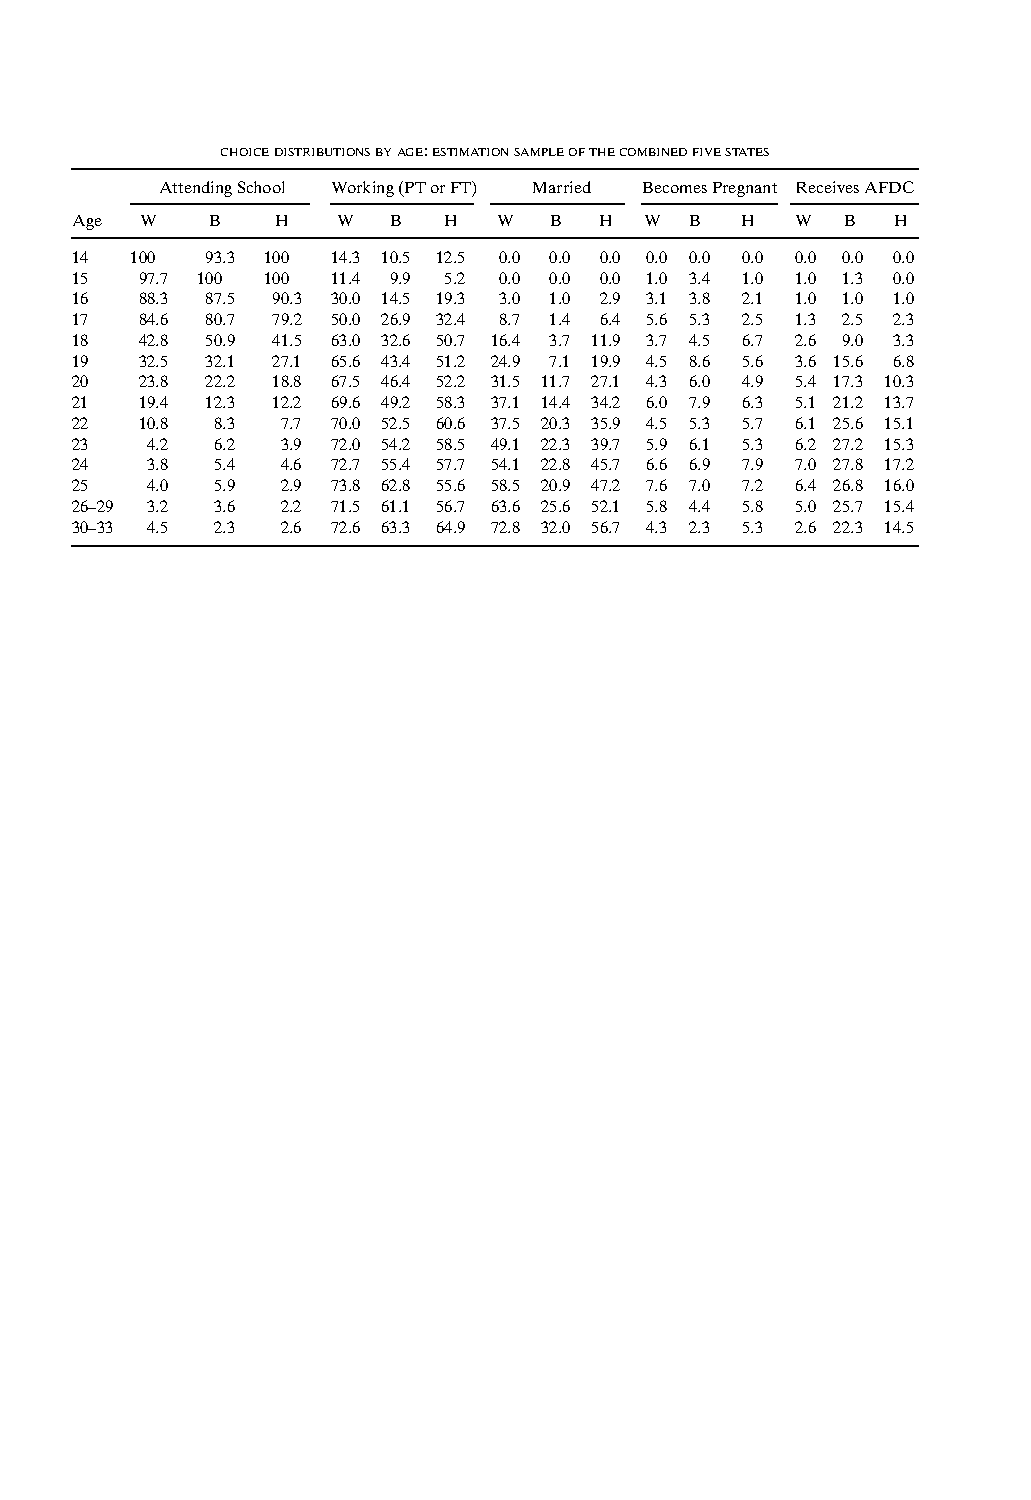
\includegraphics[width=4.5in]{tab-figs/table1_2010.pdf}
\end{frame}

\begin{frame}
	\frametitle{Estimated Monthly Benefits: Females}
	
\includegraphics[width=4.5in]{tab-figs/table2b_2010-1} \\
	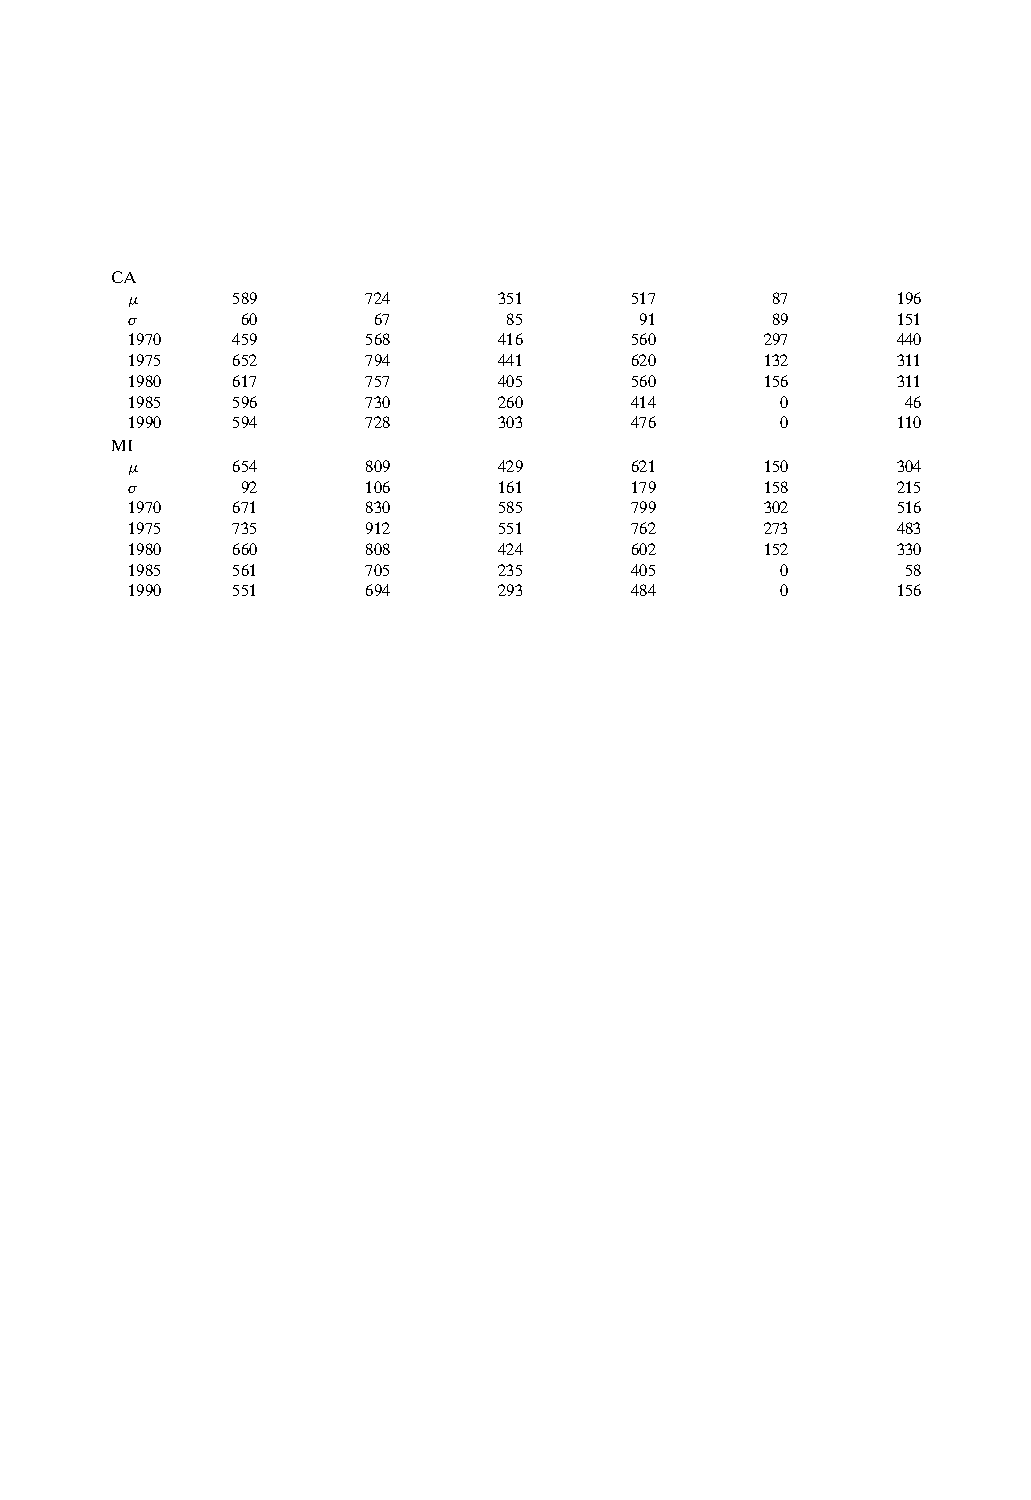
\includegraphics[width=4.5in]{tab-figs/table2a__2010.pdf} \\
	
\includegraphics[width=4.5in]{tab-figs/table2c_2010_footer}
\end{frame}

\begin{frame}
	\frametitle{Estimated Monthly Benefits (contd 1): Females}
	
\includegraphics[width=4.5in]{tab-figs/table2b_2010-1} \\
	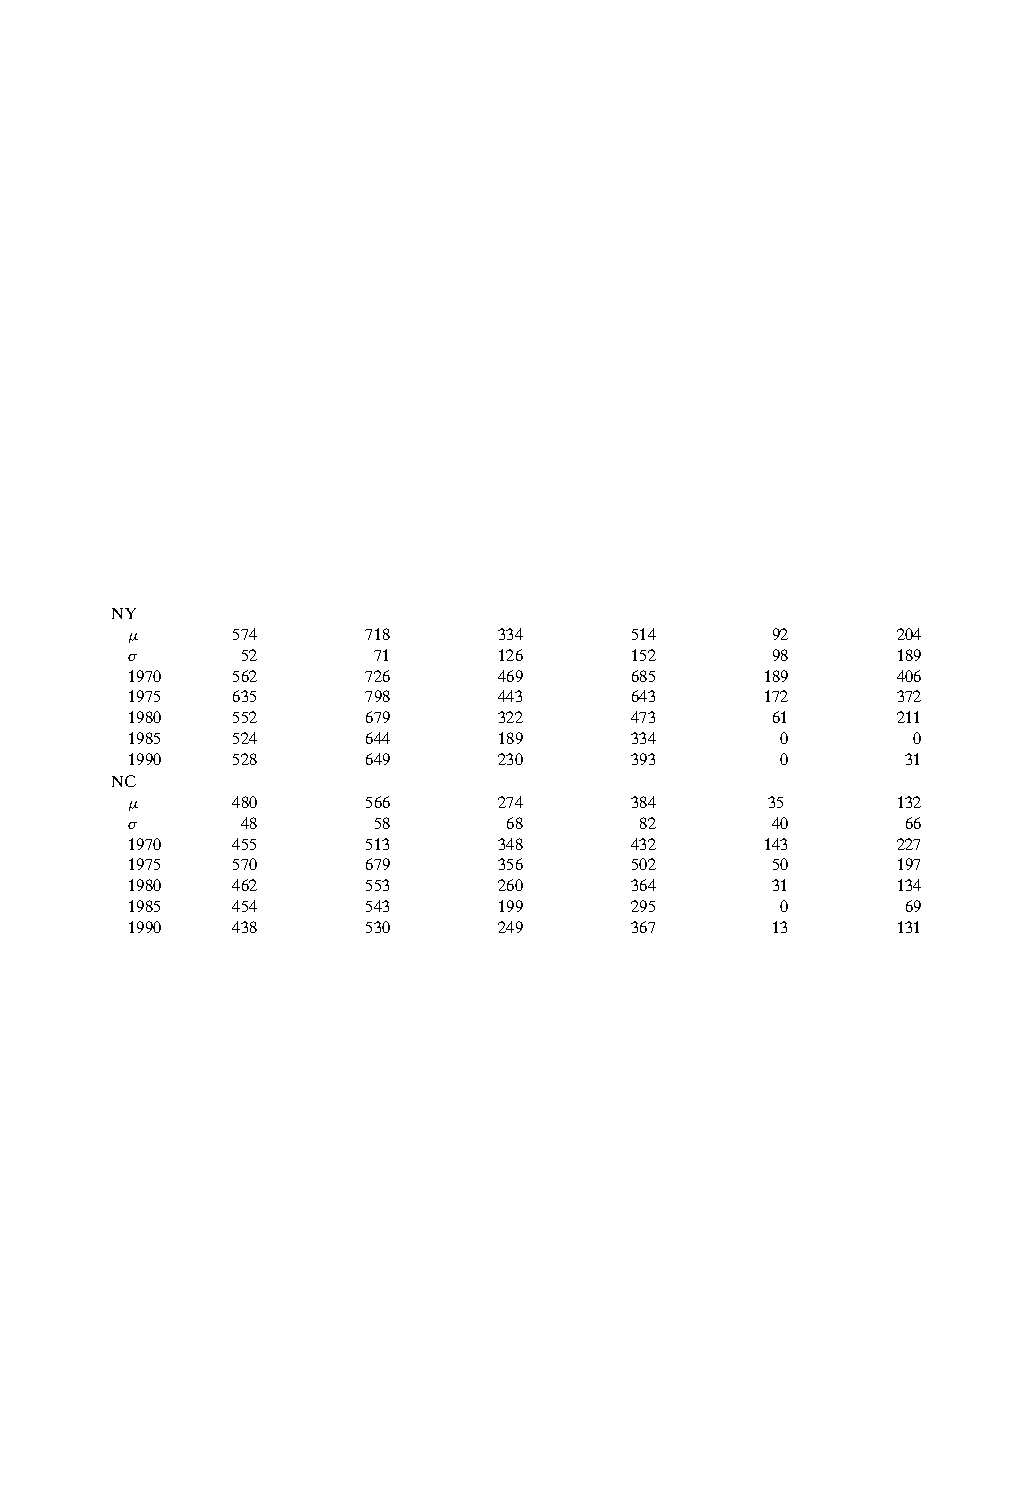
\includegraphics[width=4.5in]{tab-figs/table2b__2010} \\
	
\includegraphics[width=4.5in]{tab-figs/table2c_2010_footer}
\end{frame}

\begin{frame}
	\frametitle{Estimated Monthly Benefits (contd 2): Females}
	
\includegraphics[width=4.5in]{tab-figs/table2b_2010-1} \\
	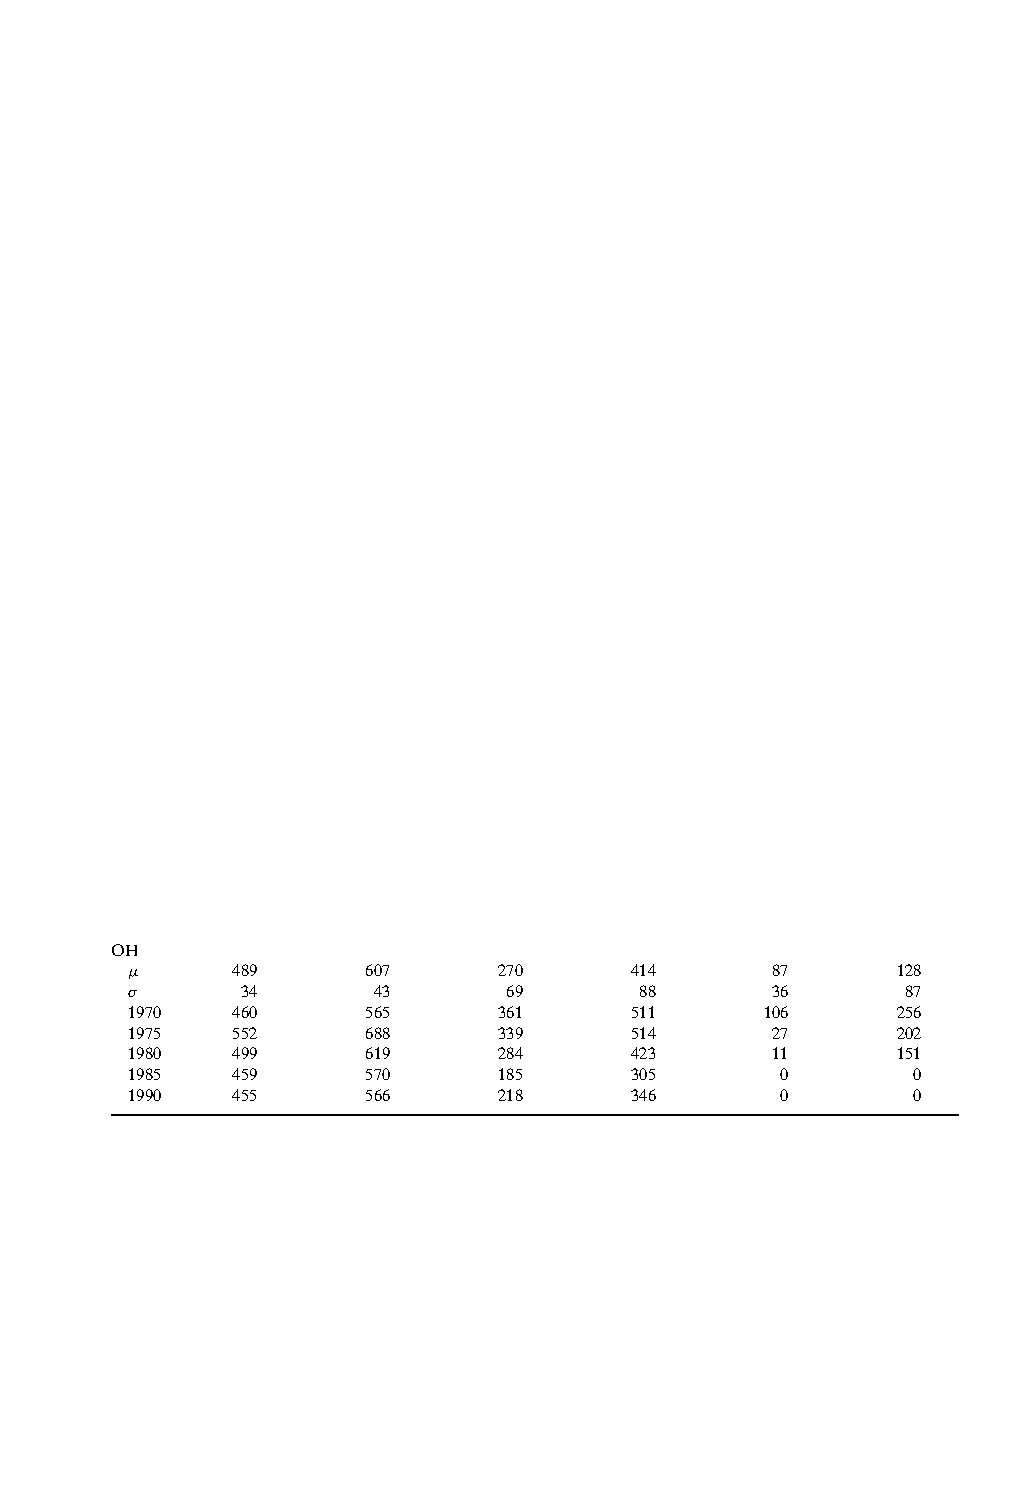
\includegraphics[width=4.5in]{tab-figs/table2c__2010}
\end{frame}

\begin{frame}
	\frametitle{Data: Males}
		\begin{itemize}
			\item NLSY79: represents the cohort of young individuals (ages $14$ to $21$) in 1979: $12,686$ total observations
			\item Focus on core white males who reach 16 years between 1977-1981
			\item Period decision: one schooling year
			\begin{itemize}
				\item Age span, 16 to 26 years old (follow up to 1988)
			\end{itemize}						
		\end{itemize}
\end{frame}

\begin{frame}
	\frametitle{Choice Distribution by Age: Males}
	\begin{center}
	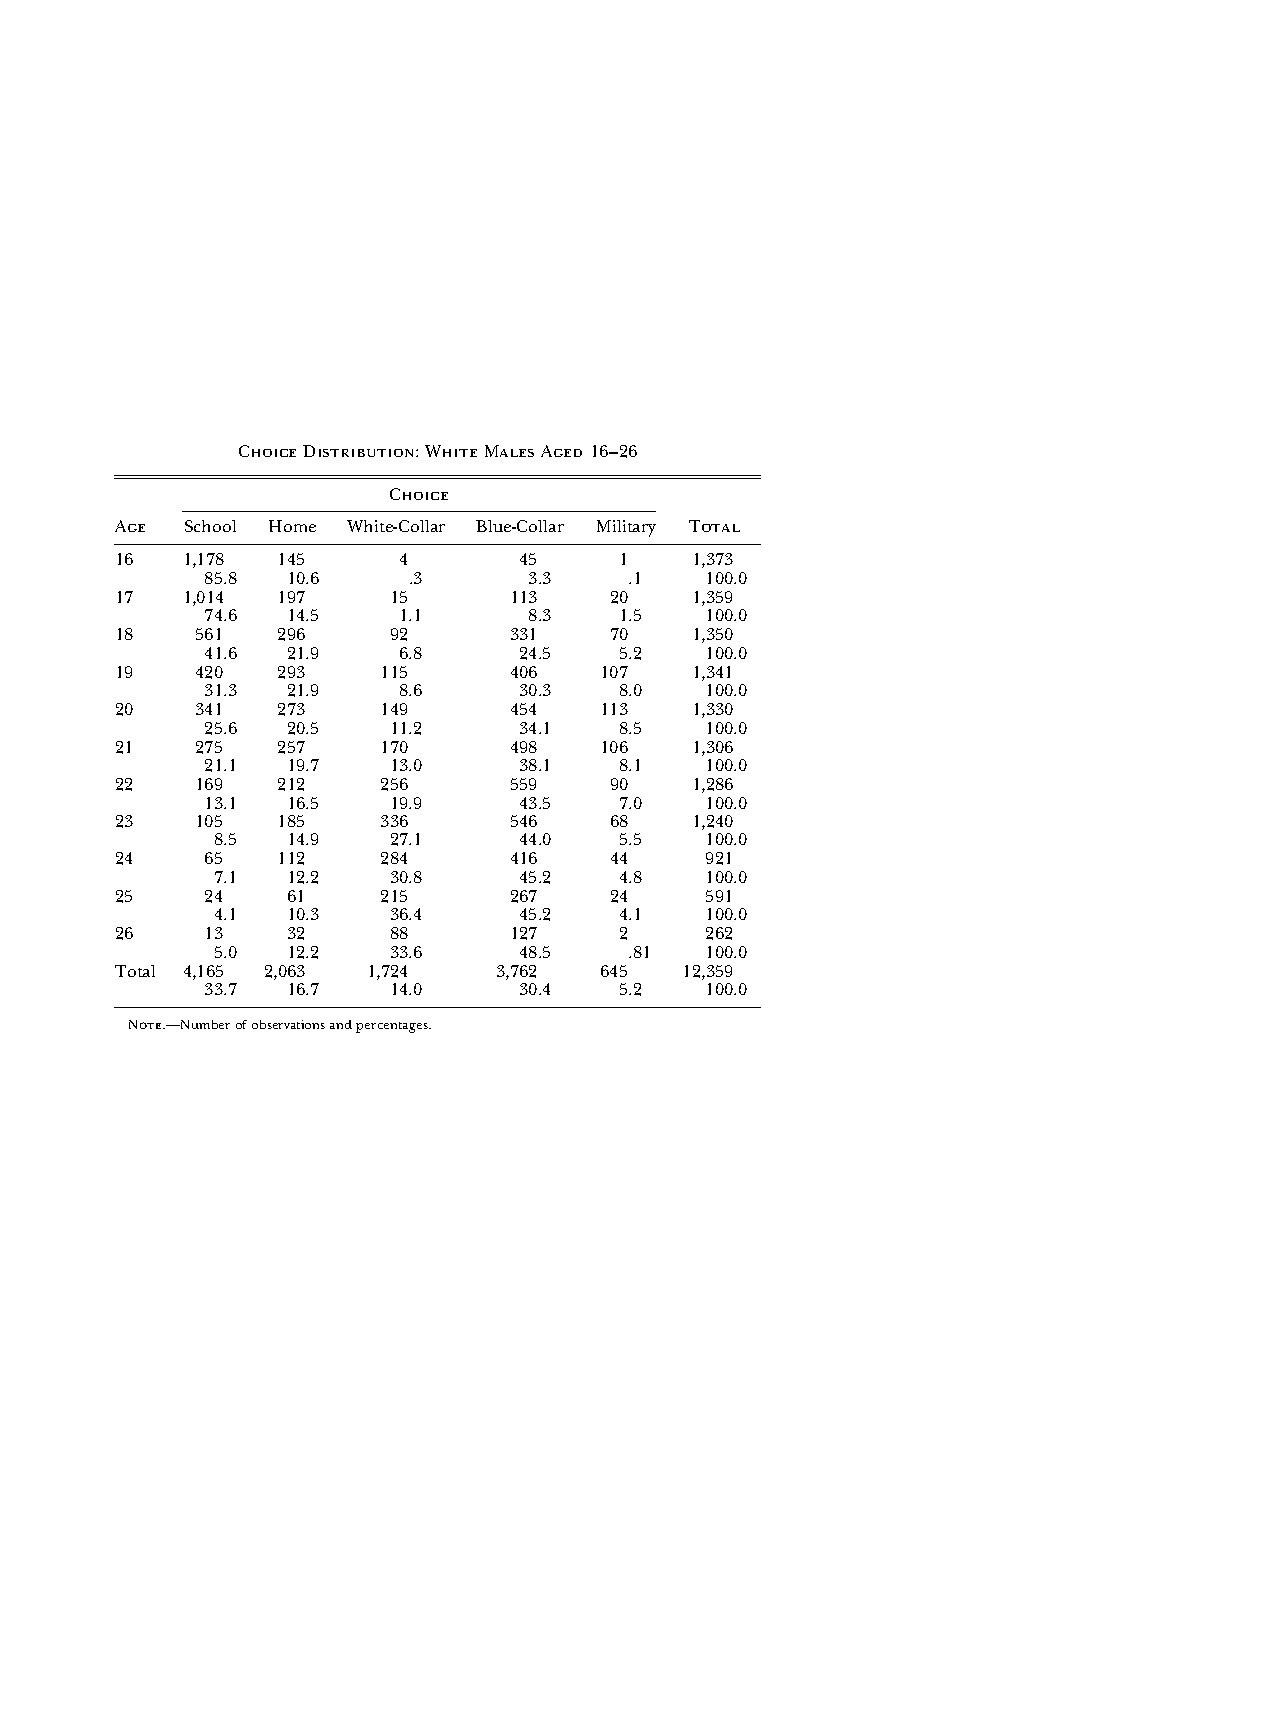
\includegraphics[width=3.5in]{tab-figs/table1_1997}
	\end{center}
\end{frame}

\begin{frame}
	\frametitle{Choice-State Combinations: Males}
	
\includegraphics{tab-figs/table3_1997_header} \\
	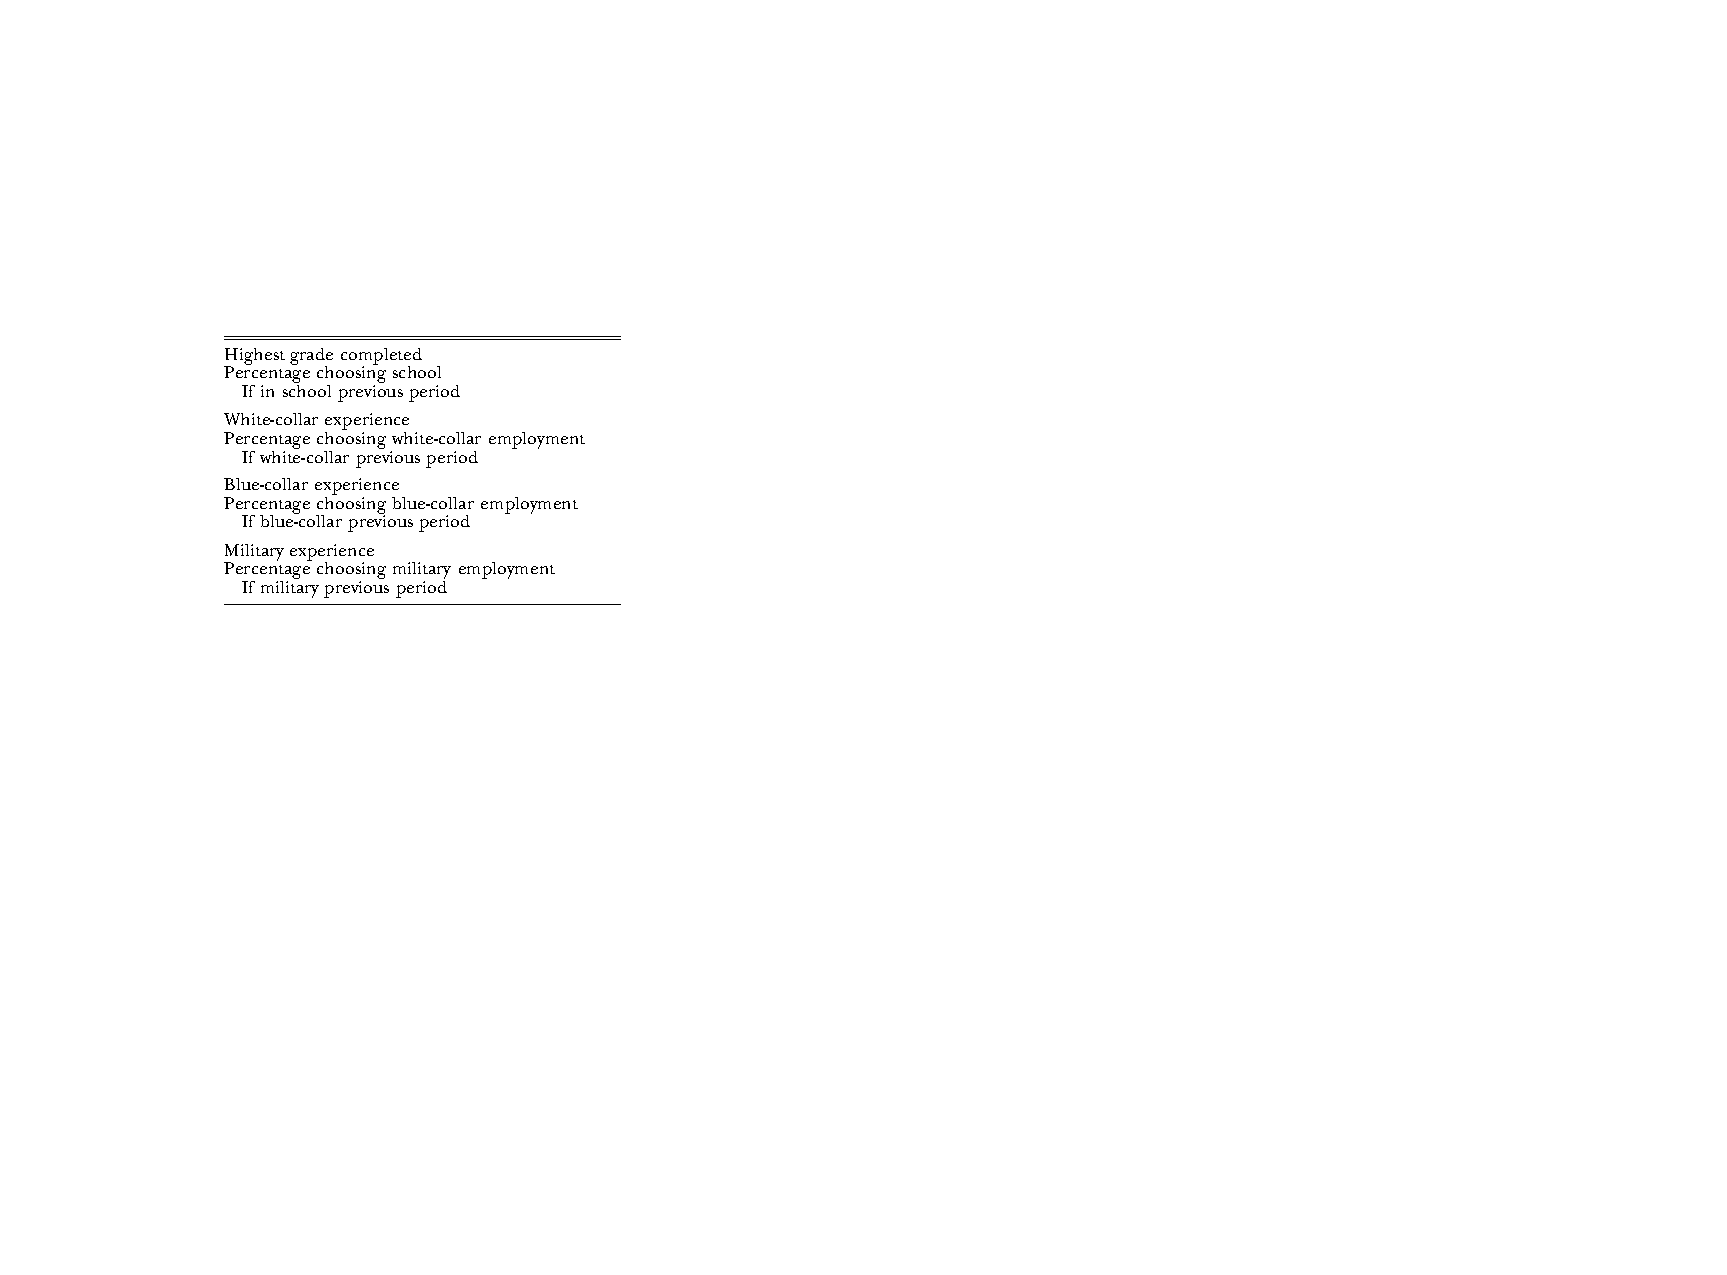
\includegraphics[height=1.75in]{tab-figs/table3_1997_left} 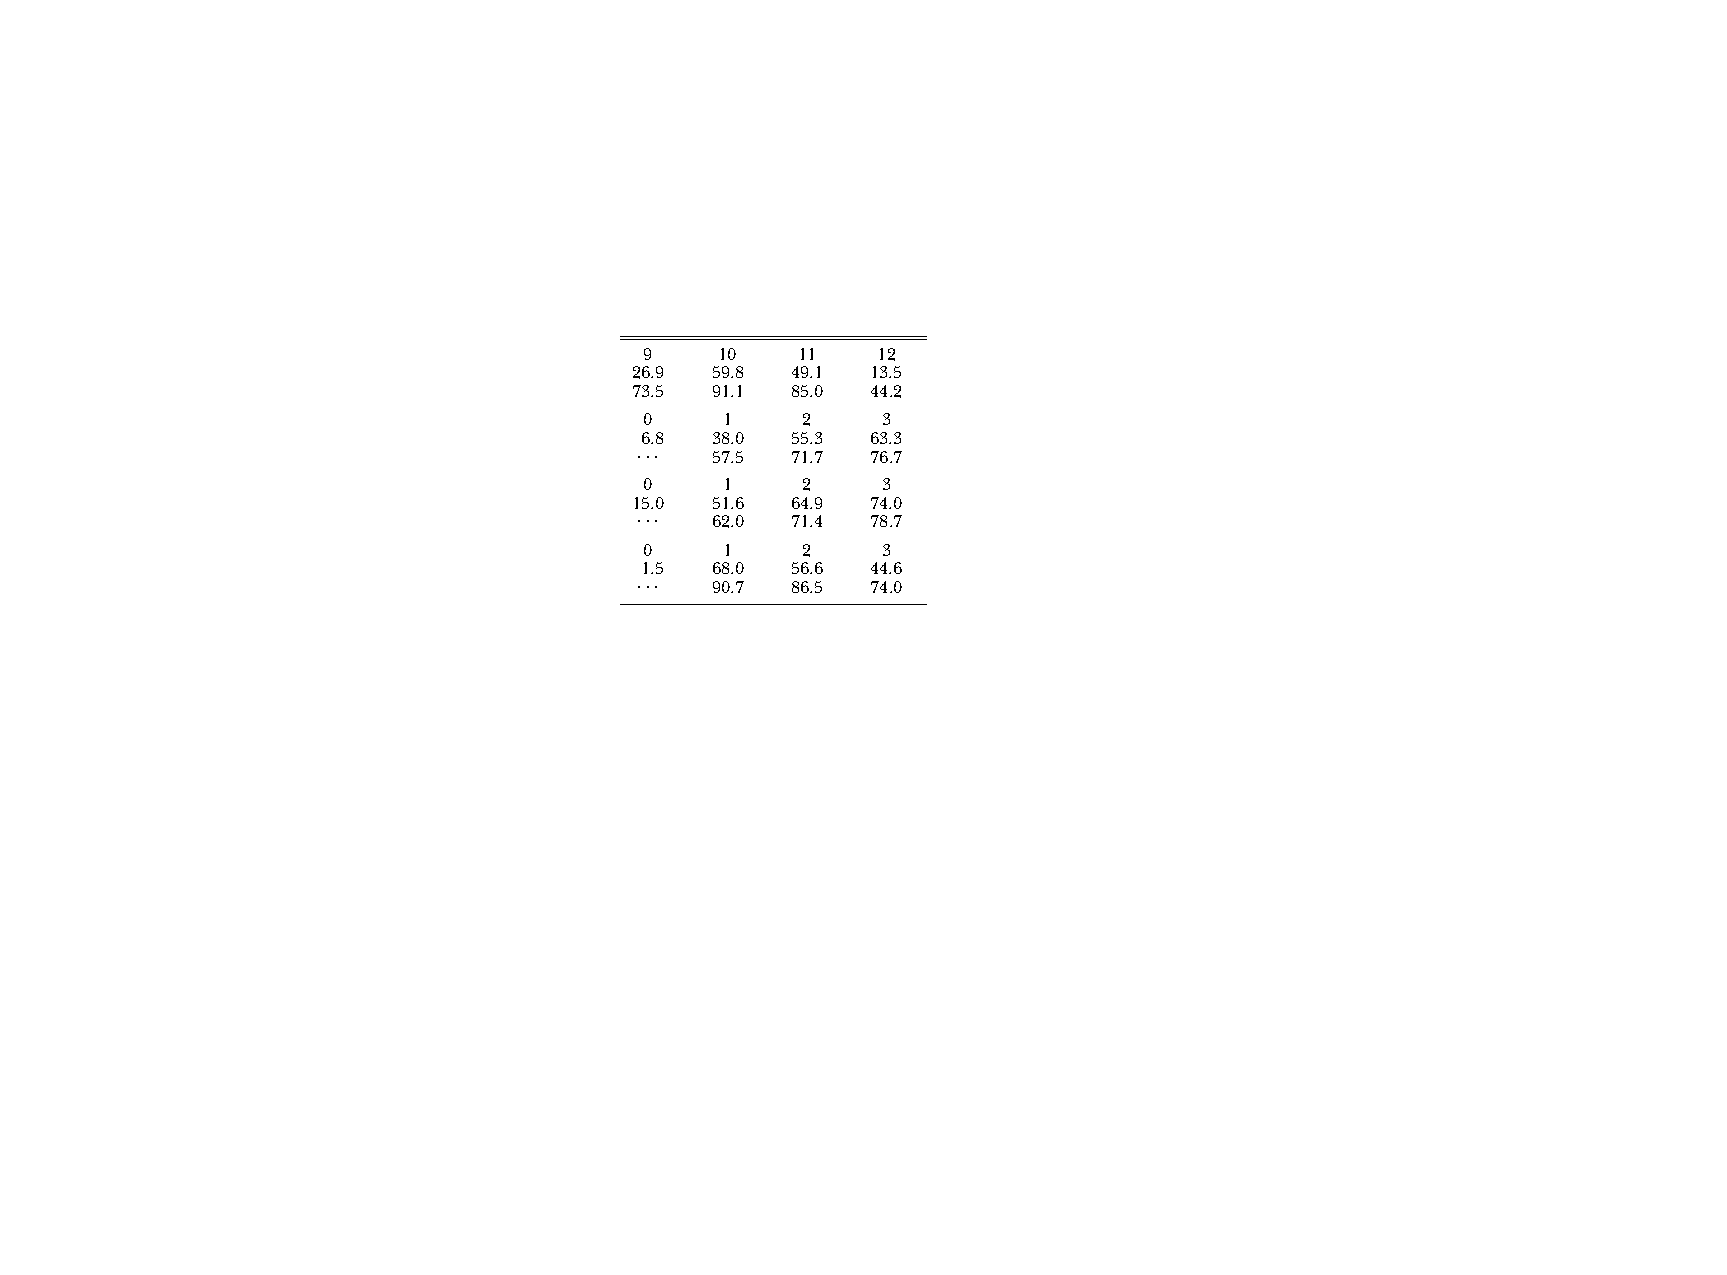
\includegraphics[height=1.75in]{tab-figs/table3a_1997}
\end{frame}

\begin{frame}
	\frametitle{Choice-State Combinations (contd): Males}
	
\includegraphics{tab-figs/table3_1997_header} \\
	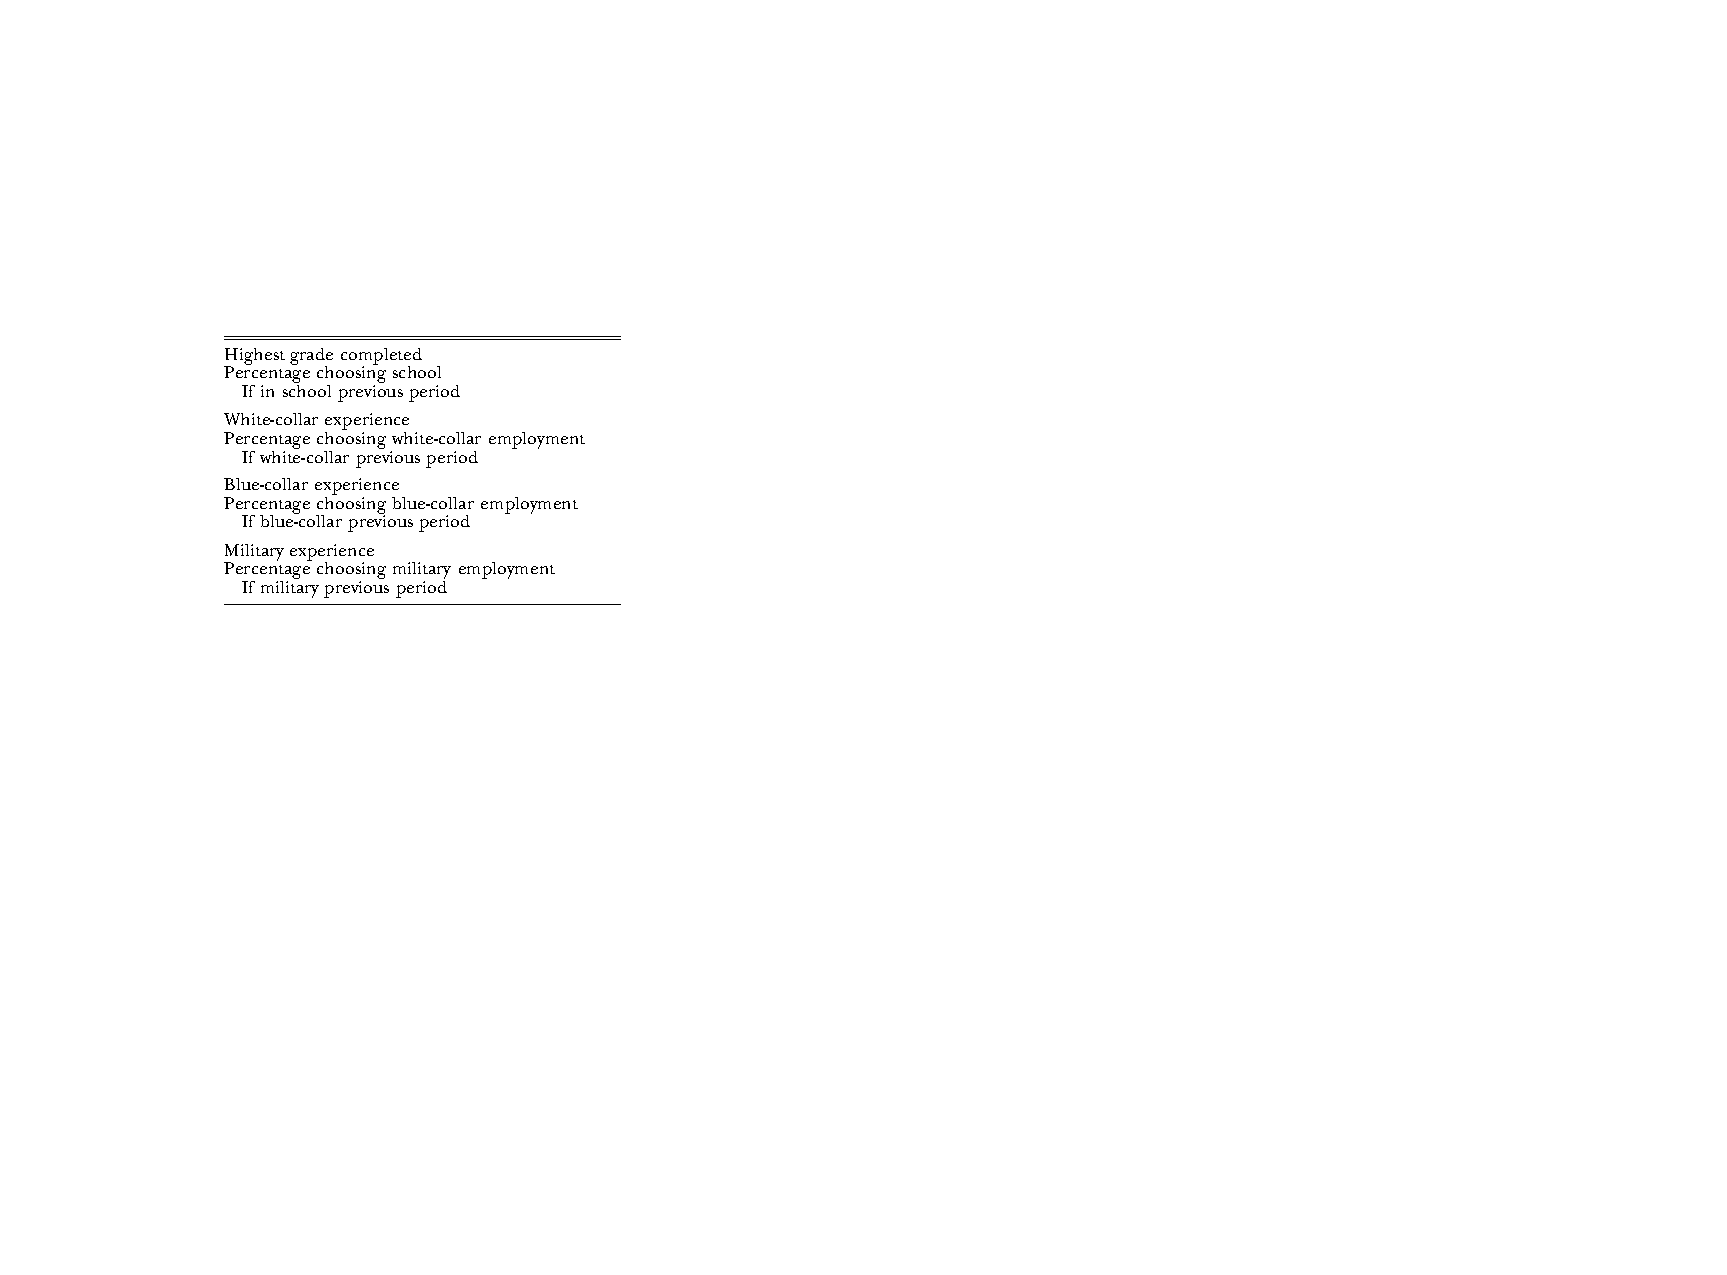
\includegraphics[height=1.5in]{tab-figs/table3_1997_left} 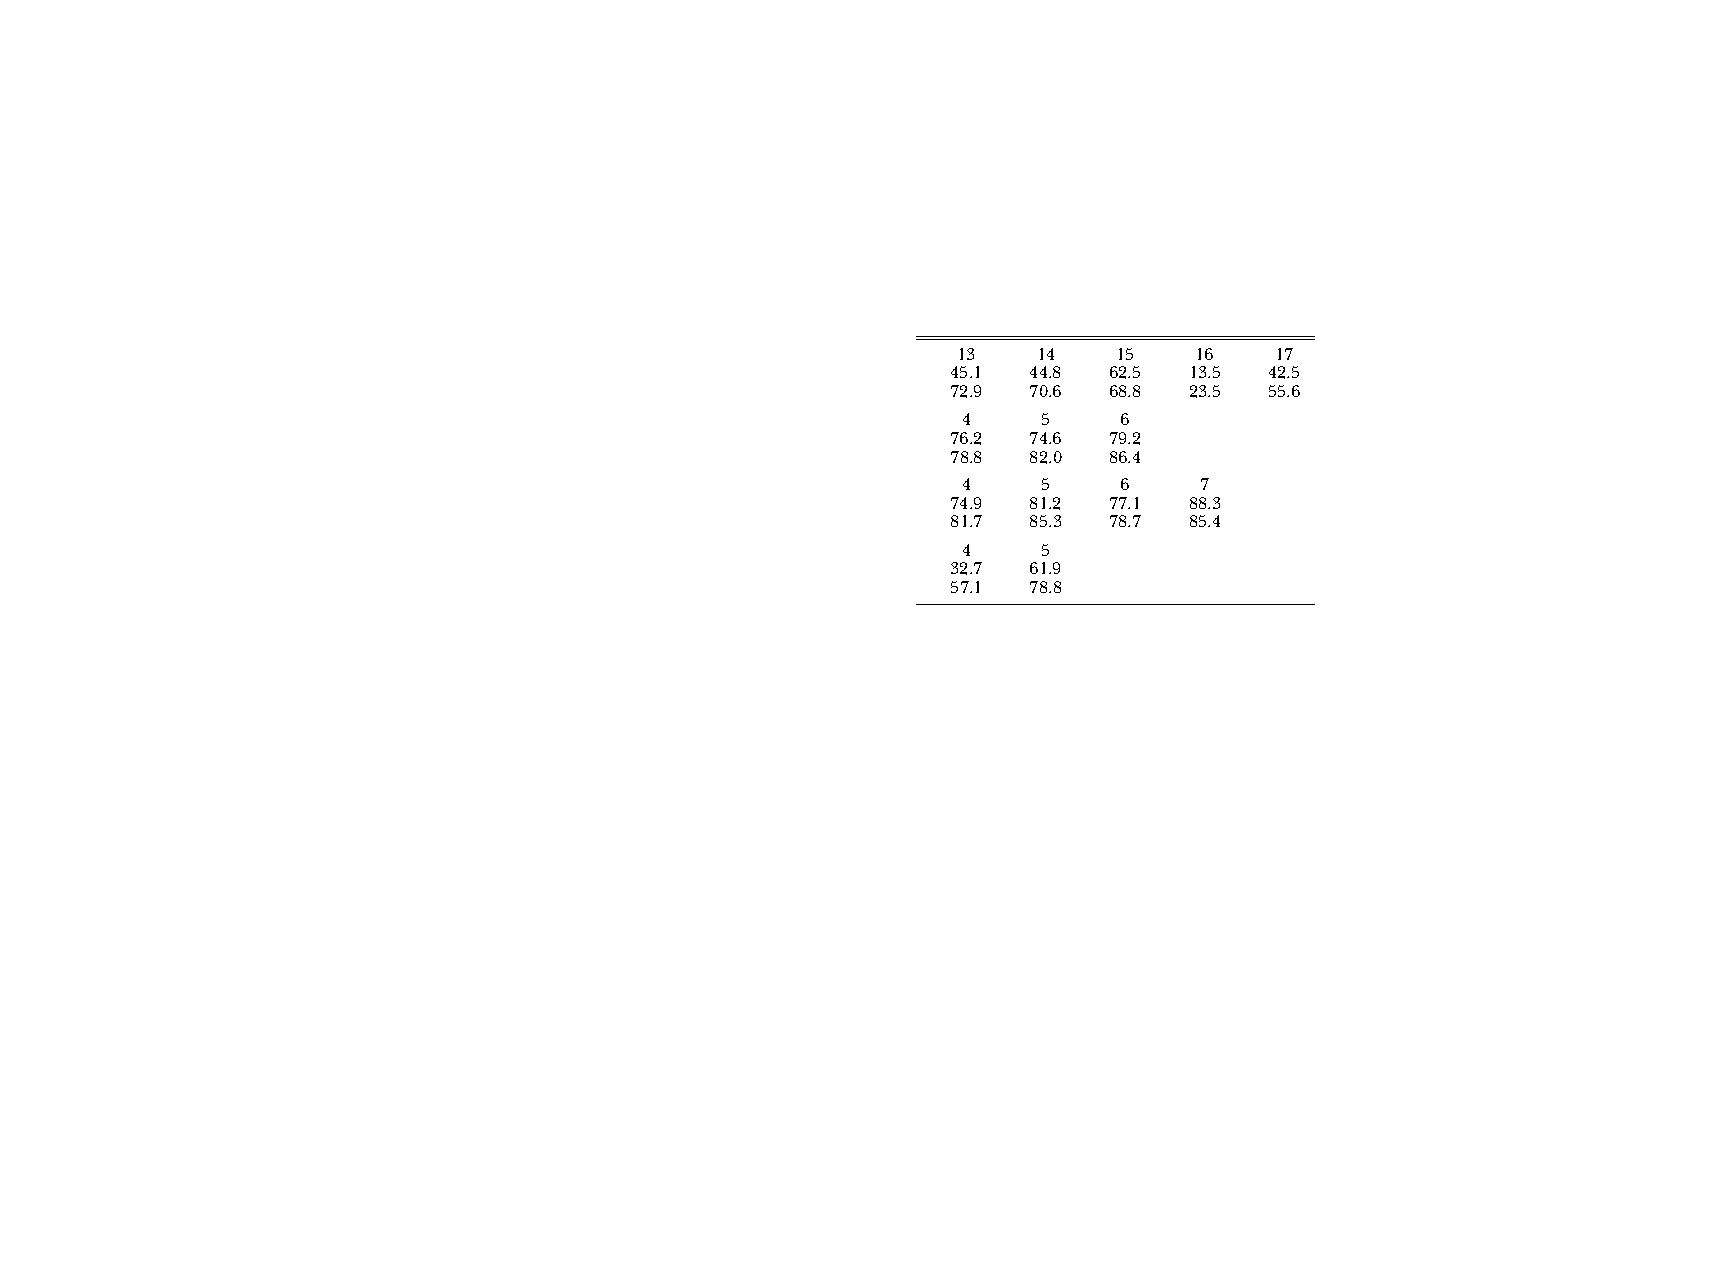
\includegraphics[height=1.5in]{tab-figs/table3b_1997}
\end{frame}

\begin{frame}
	\frametitle{Average Real Wages: Males}
	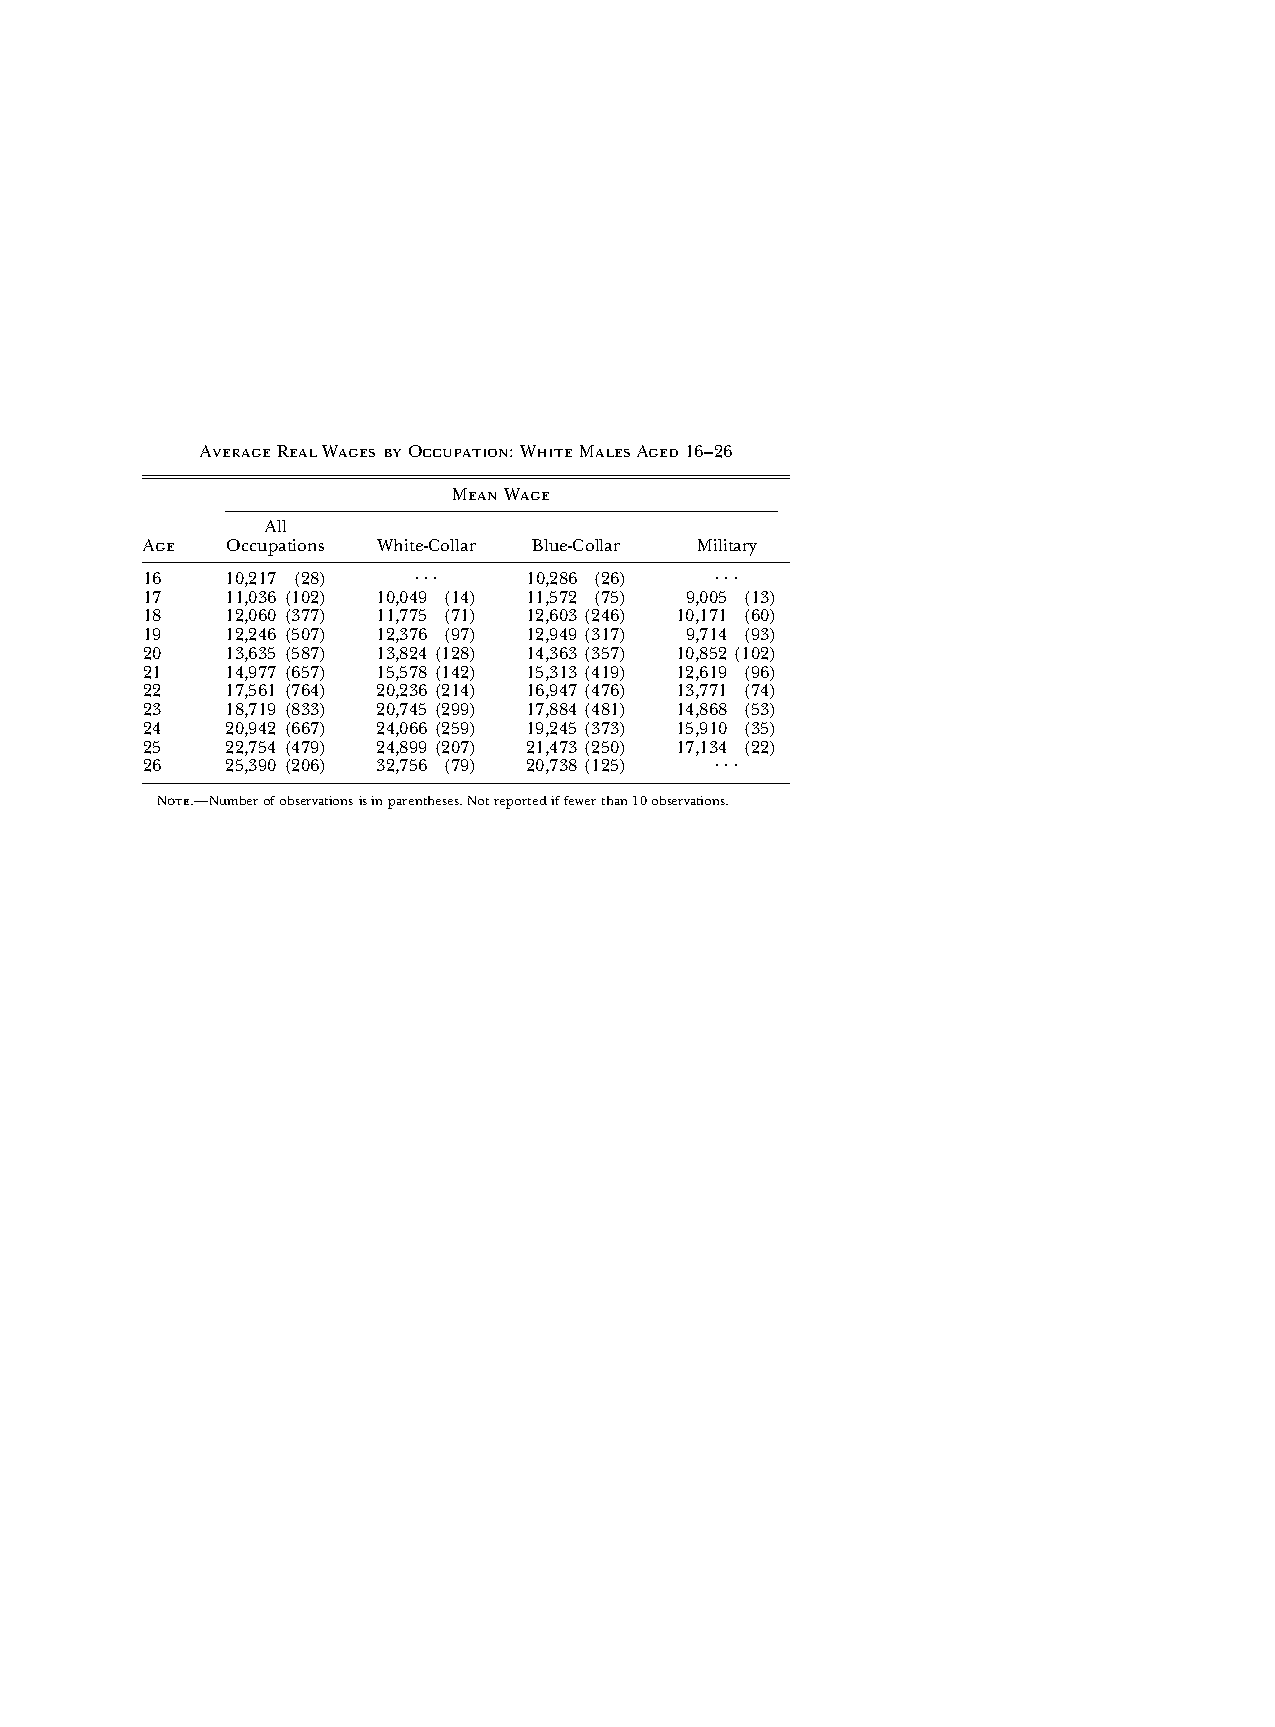
\includegraphics{tab-figs/table4_1997}
\end{frame}


\section{Estimation}

\begin{frame}
	\frametitle{Estimation Approach: Females}
		\begin{itemize}
			\item Usual estimation approach of DCDP models: simulated conditional likelihood
			\item Issues in this context:
				\begin{itemize}
					\item Requires conditional probability agent makes observed choice at $t$ given $\Omega_{a}$ at $t$
					\item Lack of complete histories of employment, schooling, and welfare for most cohorts back to age $14$
					\item Unobserved initial conditions and unobserved state variables pose DCCP estimation problems (Heckman, 1981)
					\item Need to integrate over distribution of unobserved elements: intractably complex
					\item Estimate based on unconditional simulation of the likelihood function based on the (realistic) assumption that all outcome variables have measurement error (Keane and Wolpin, 2001)
				\end{itemize}							
		\end{itemize}
\end{frame}

\begin{frame}
	\frametitle{Estimation Approach: Males}
		\begin{itemize}
			\item Simulated conditional likelihood
			\item ``Easy'' to write and calculate the likelihood function:
			\begin{equation}
				\Pr \left( c(16), \ldots, c(\bar{a})|g_{n}(16) \right) =
\sum \limits _{k=1} ^K \prod \limits _{a=16} ^{\bar{a}} \pi_{k|g(16)} L_{nk} \nonumber
			\end{equation}
\noindent with
\begin{equation}
L_{nk} = \Pr \left( c_{n}(a) | g_n(16), \text{type=k} \right)	\nonumber 
\end{equation}
\noindent where $k=1,\ldots,K$ and $n = 1, \ldots, N$ index types and individuals, respectively. $\pi_{k|g_{n}(16)}$ are type proportions, and $c_{n}(a)$ is a choice-reward combination
		\end{itemize}
\end{frame}

\begin{frame}
	\frametitle{Model Fit and External Validation: Females}
		\begin{itemize}
			\item Keane and Wolpin (2007) studies this  extensively:
				\begin{itemize}
					\item Within sample fit: captures features of the data well (choice frequencies and welfare use for each group in each state over the life cycle)
					\item External Validation: outperforms MNL with less parameters ($202$ vs $240$) in external validation exercises: 
					\begin{itemize}
						\item Forecast behavior of women in TX
						\item What happens if estimation states adopt TX's welfare system?
					\end{itemize}
				\end{itemize}
		\end{itemize}				
\end{frame}

\begin{frame}
	\frametitle{Model Fit and External Validation: Males}
		\begin{itemize}
			\item Within-sample: Figures 1-5 evidence satisfactory within-sample fit, which is confirmed through tests (Table 5)
			\item External validation: model frequency predictions coincide with CPS choice frequencies (Table 10)
		\end{itemize}
\end{frame}

\begin{frame}
	\frametitle{Model Fit and External Validation (contd 1): Males}
	\begin{center}
	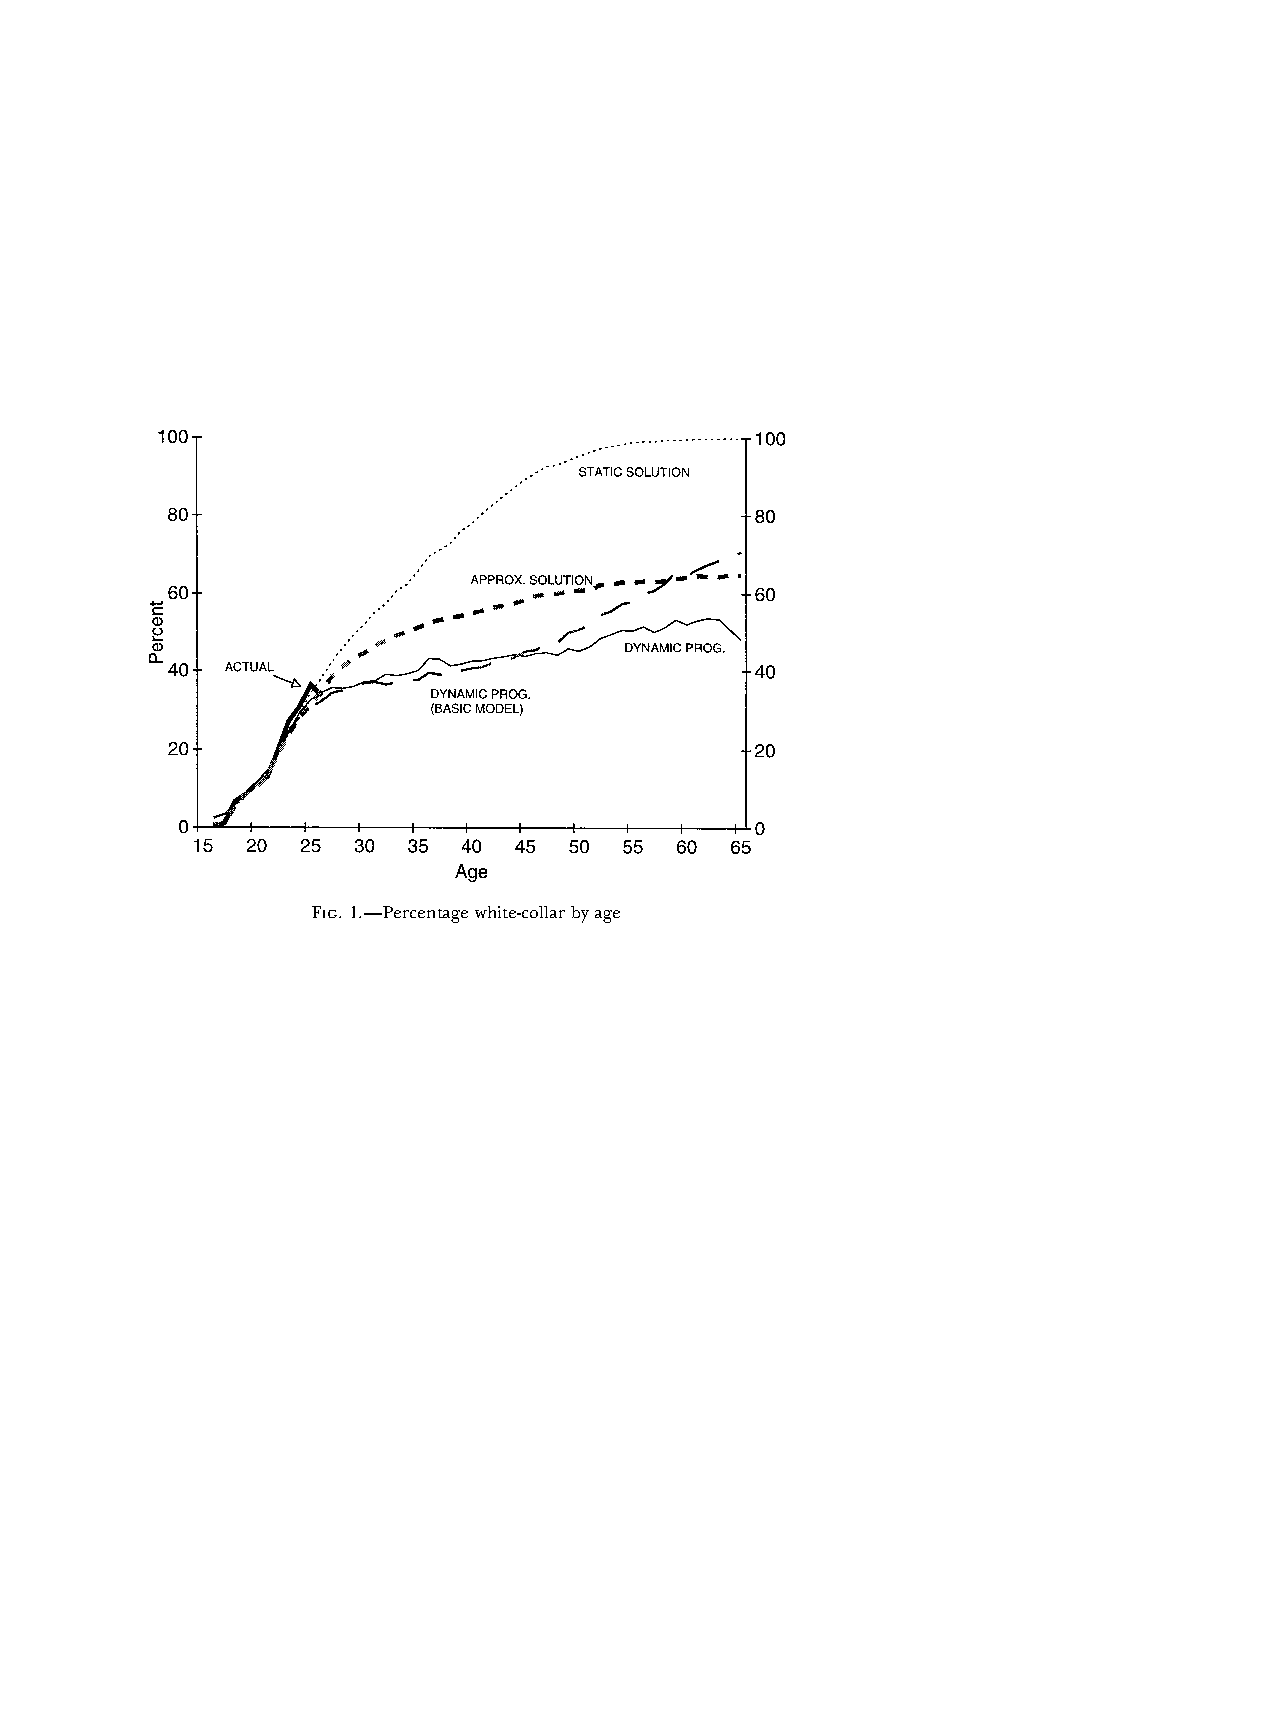
\includegraphics[width=.9\textwidth]{tab-figs/figure1_1997}
	\end{center}
\end{frame}

\begin{frame}
	\frametitle{Model Fit and External Validation (contd 2): Males}
	\begin{center}
	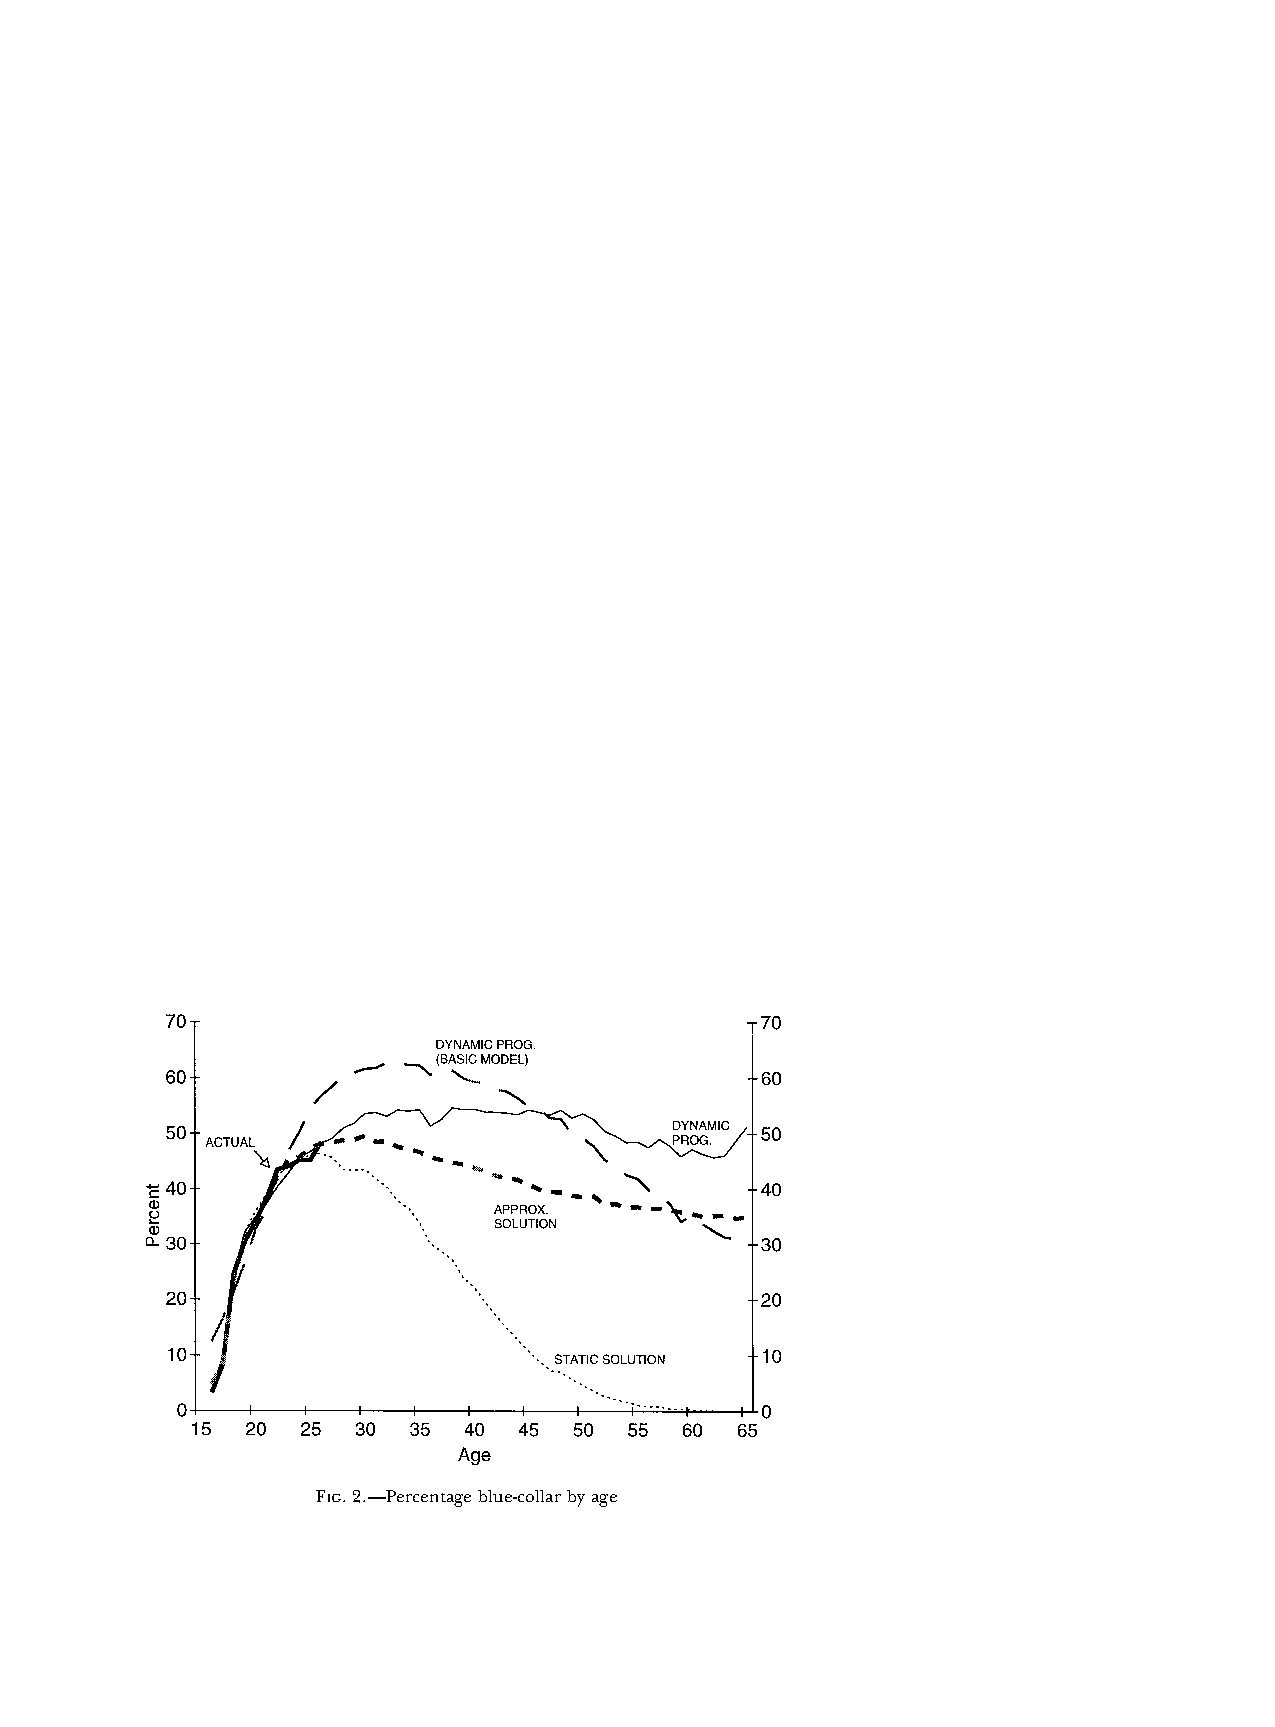
\includegraphics[width=.9\textwidth]{tab-figs/figure2_1997}
	\end{center}
\end{frame}

\begin{frame}
	\frametitle{Model Fit and External Validation (contd 3): Males}
	\begin{center}
	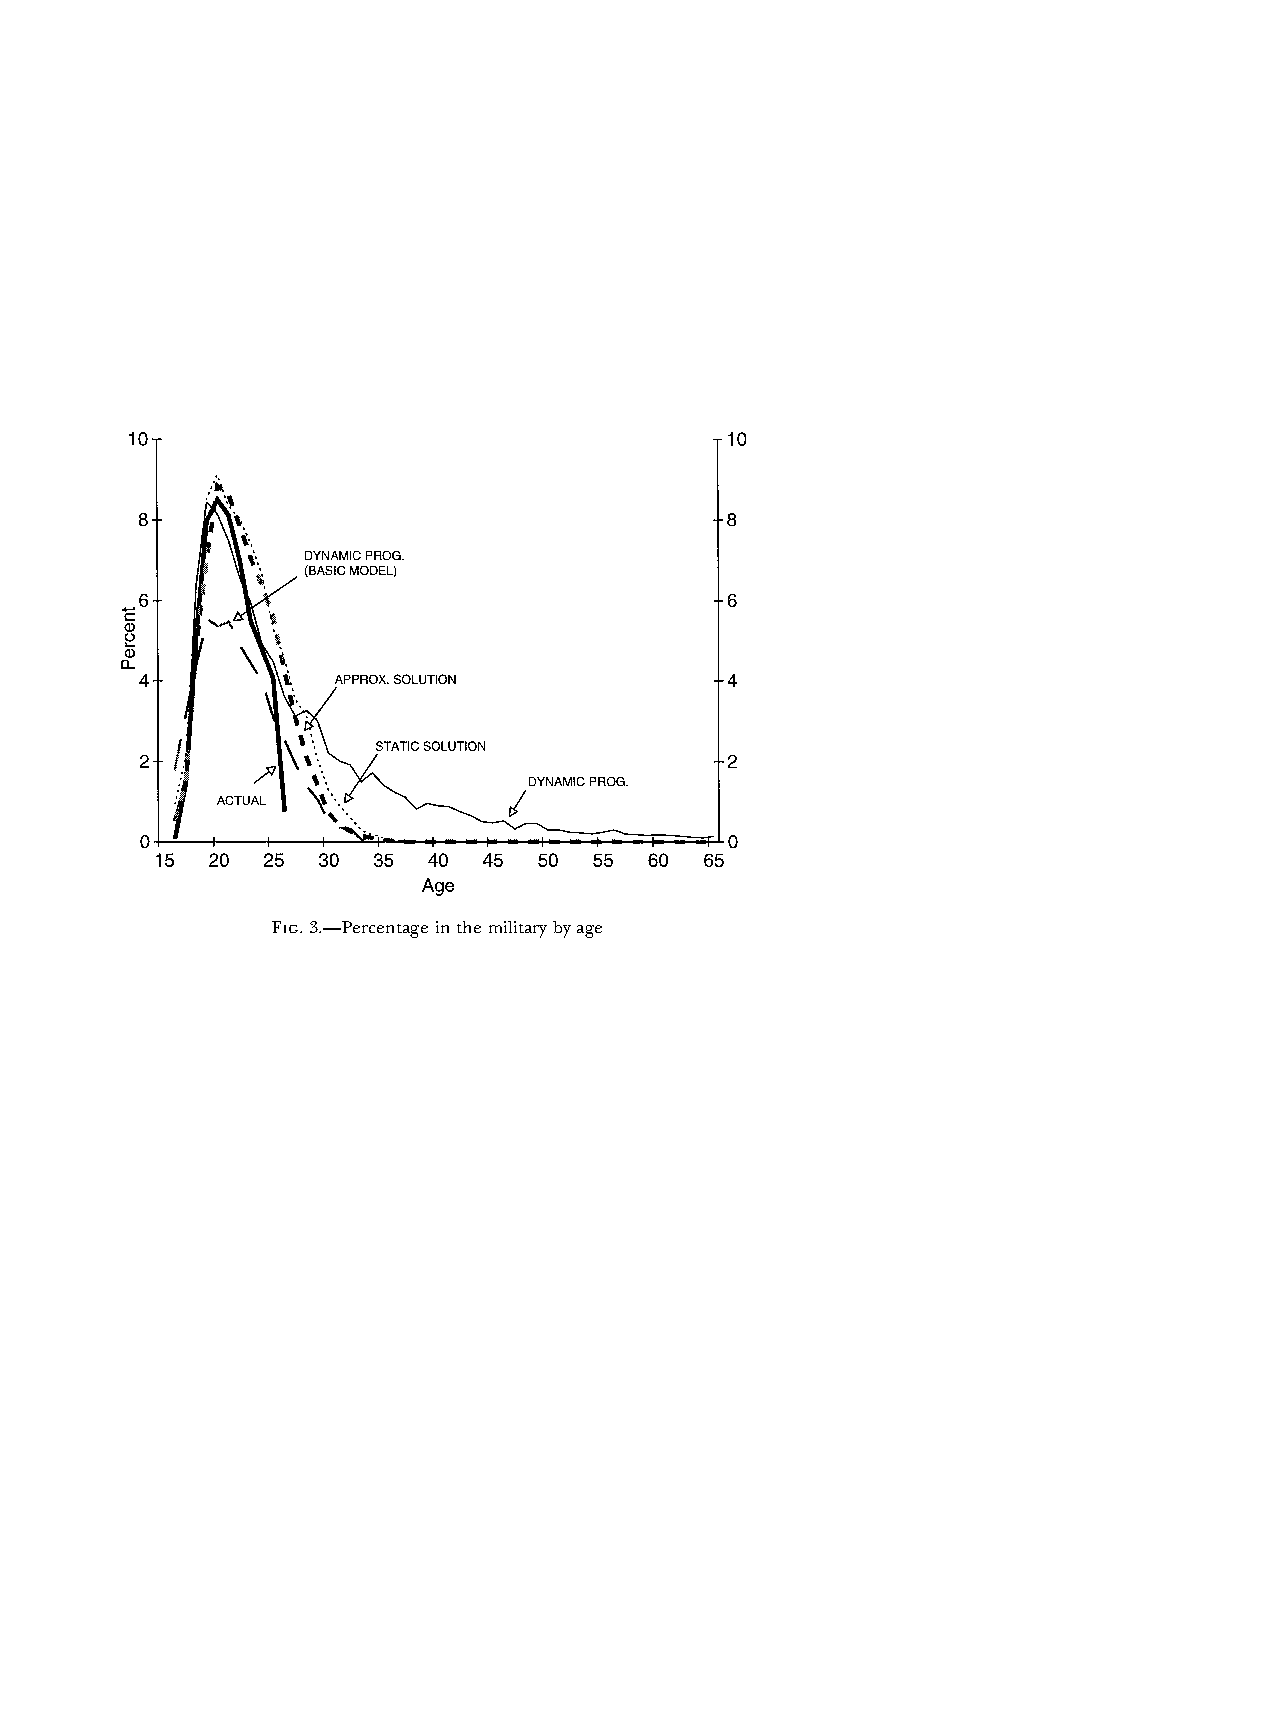
\includegraphics[width=.9\textwidth]{tab-figs/figure3_1997}
	\end{center}
\end{frame}

\begin{frame}
	\frametitle{Model Fit and External Validation (contd 4): Males}
	\begin{center}
	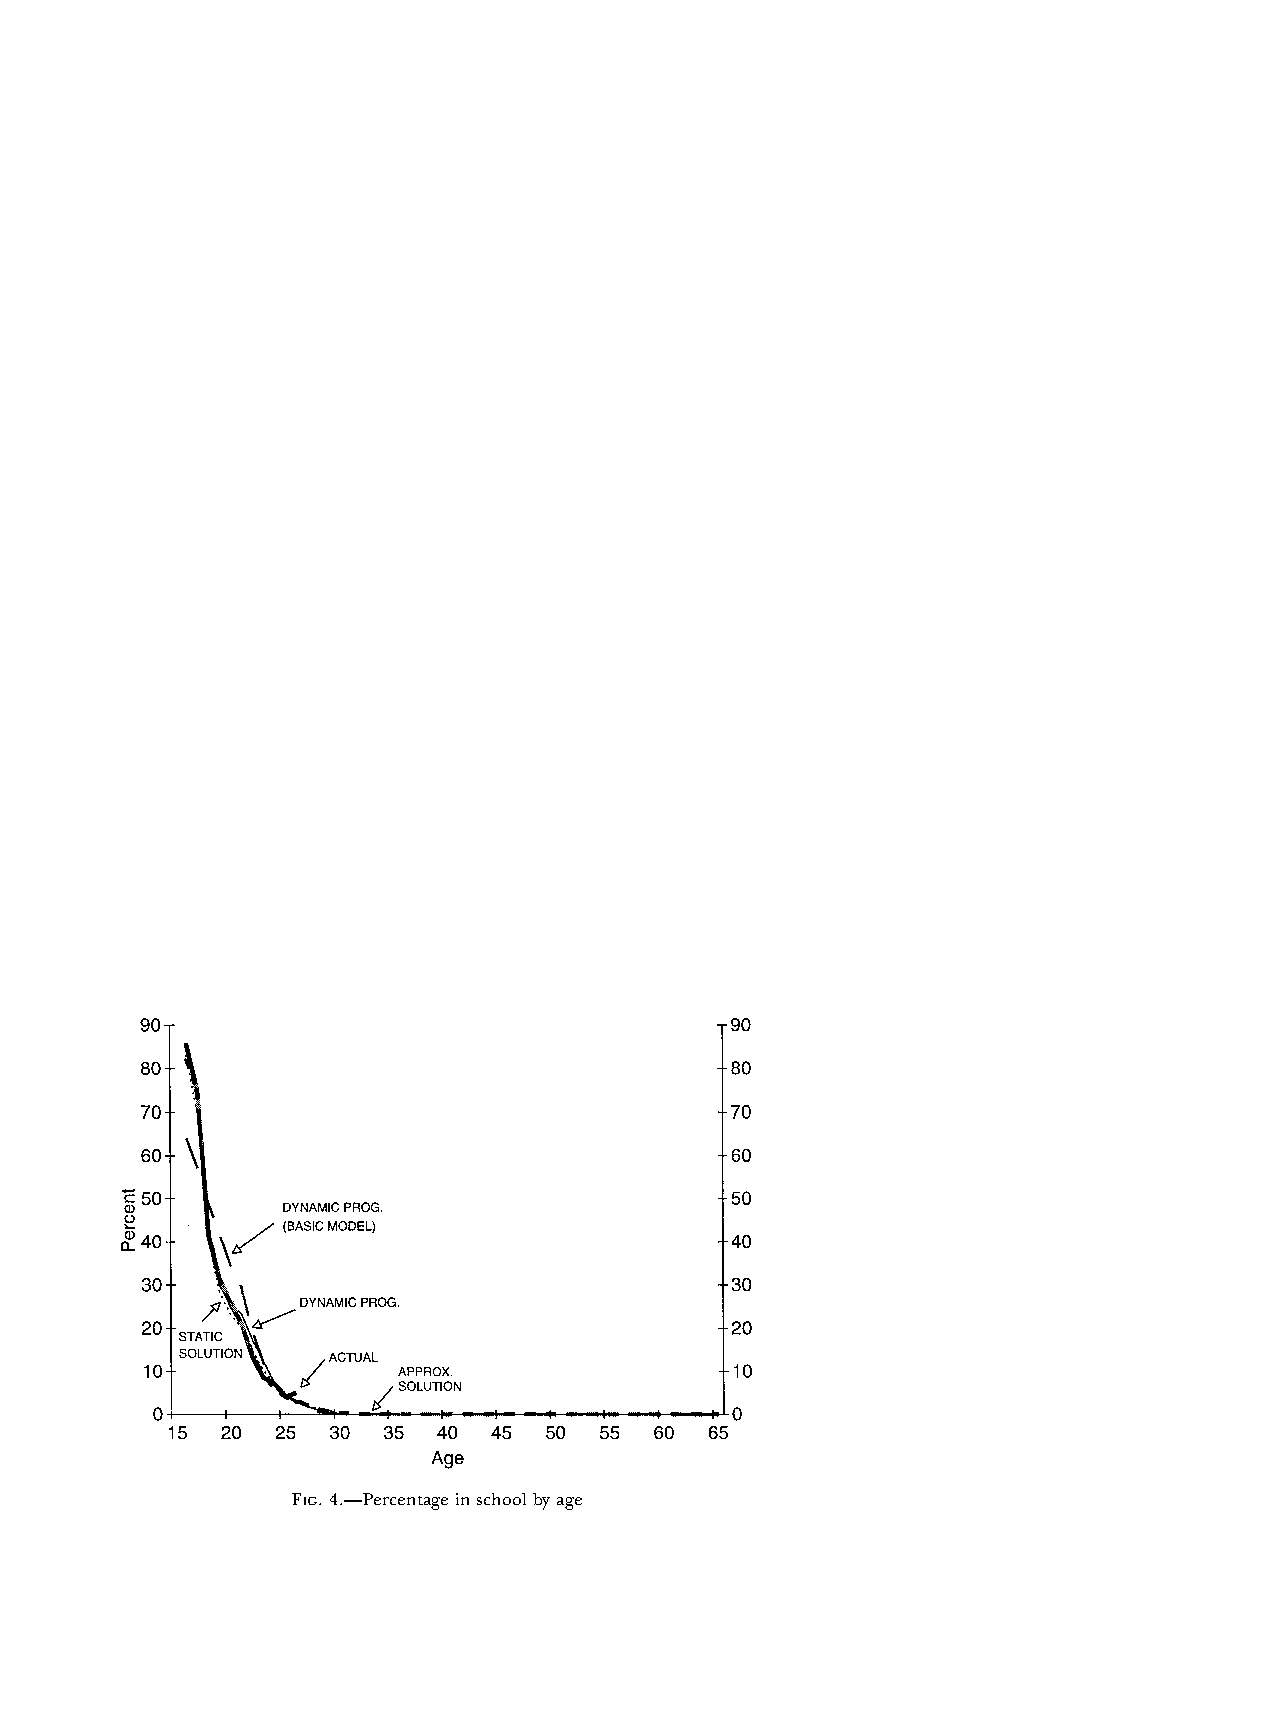
\includegraphics[width=.9\textwidth]{tab-figs/figure4_1997}
	\end{center}
\end{frame}

\begin{frame}
	\frametitle{Model Fit and External Validation (contd 5): Males}
	\begin{center}
	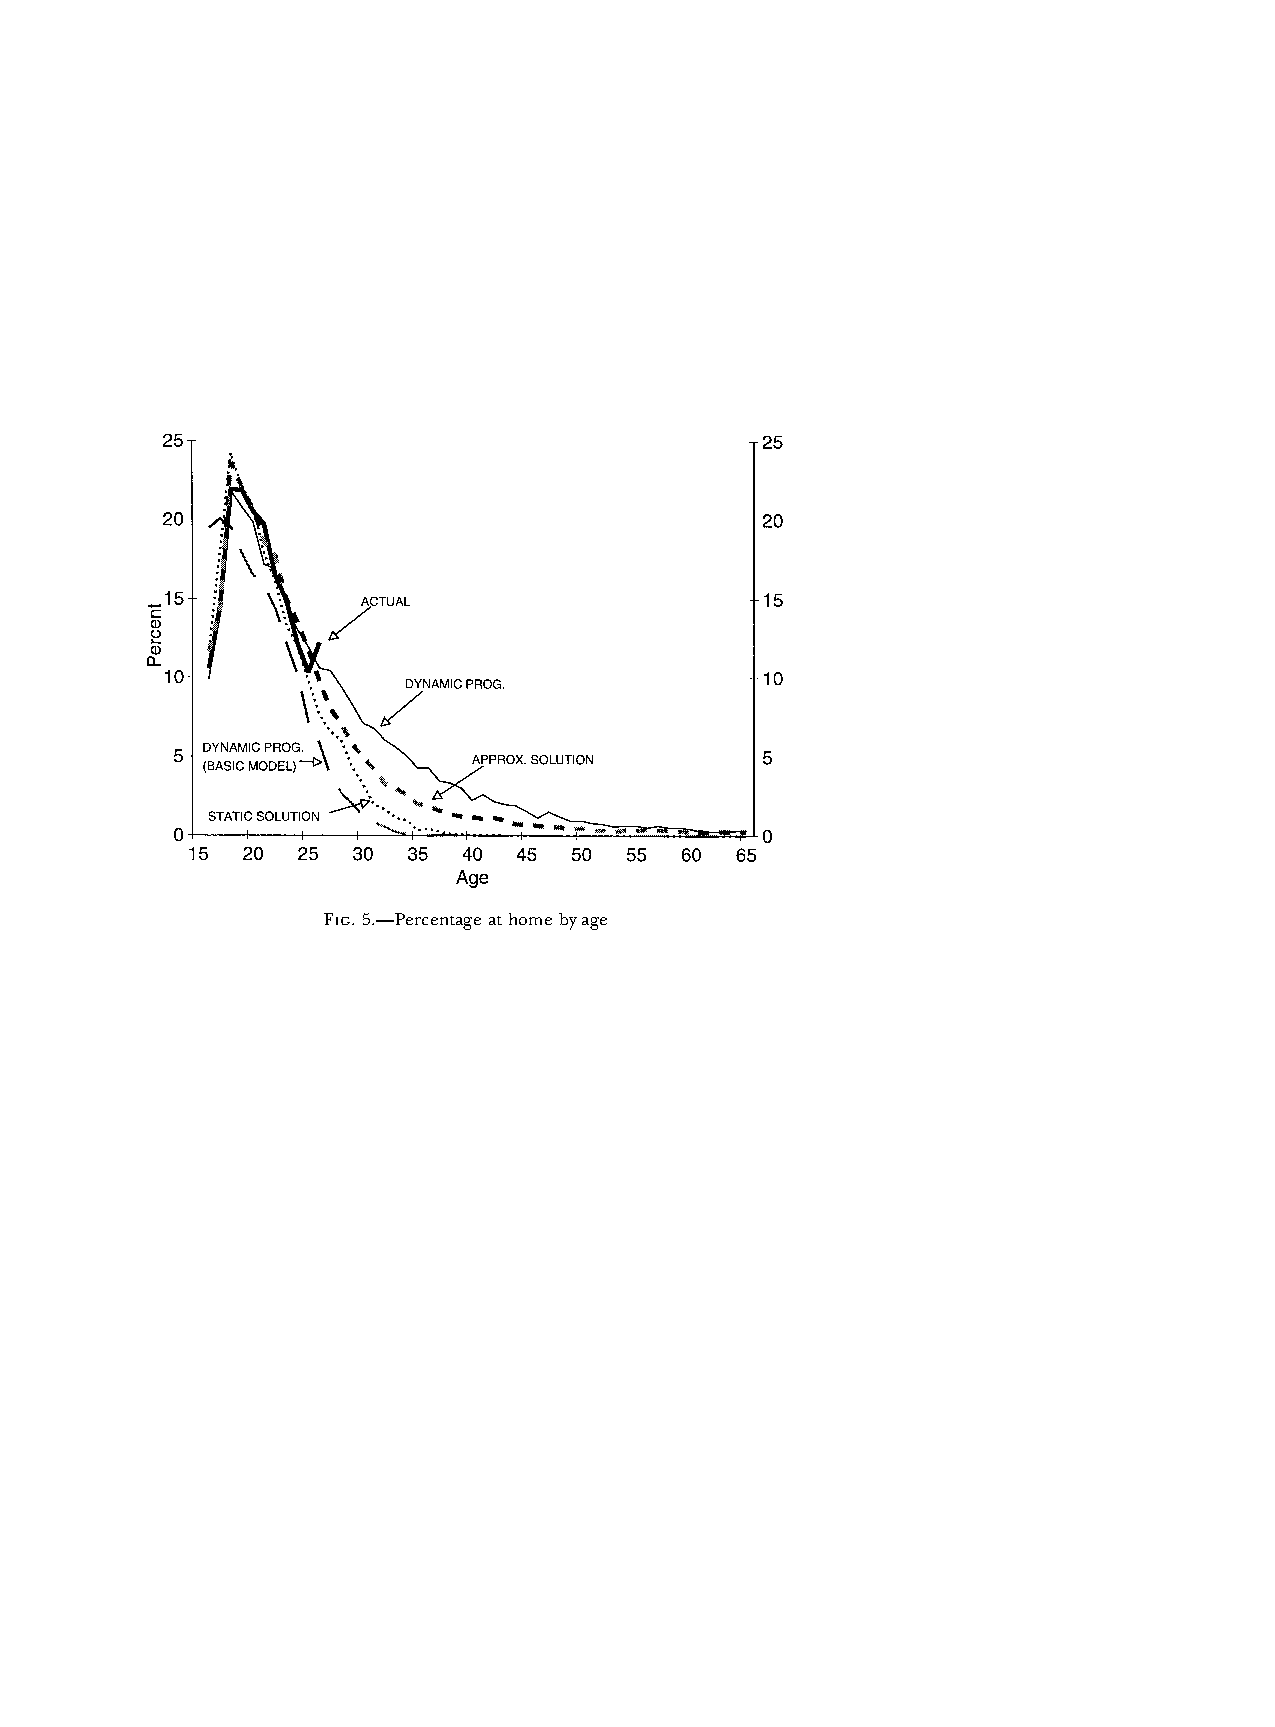
\includegraphics[width=.9\textwidth]{tab-figs/figure5_1997}
	\end{center}
\end{frame}

\begin{frame}
	\frametitle{Model Fit and External Validation (contd 6): Males}
	\begin{center}
	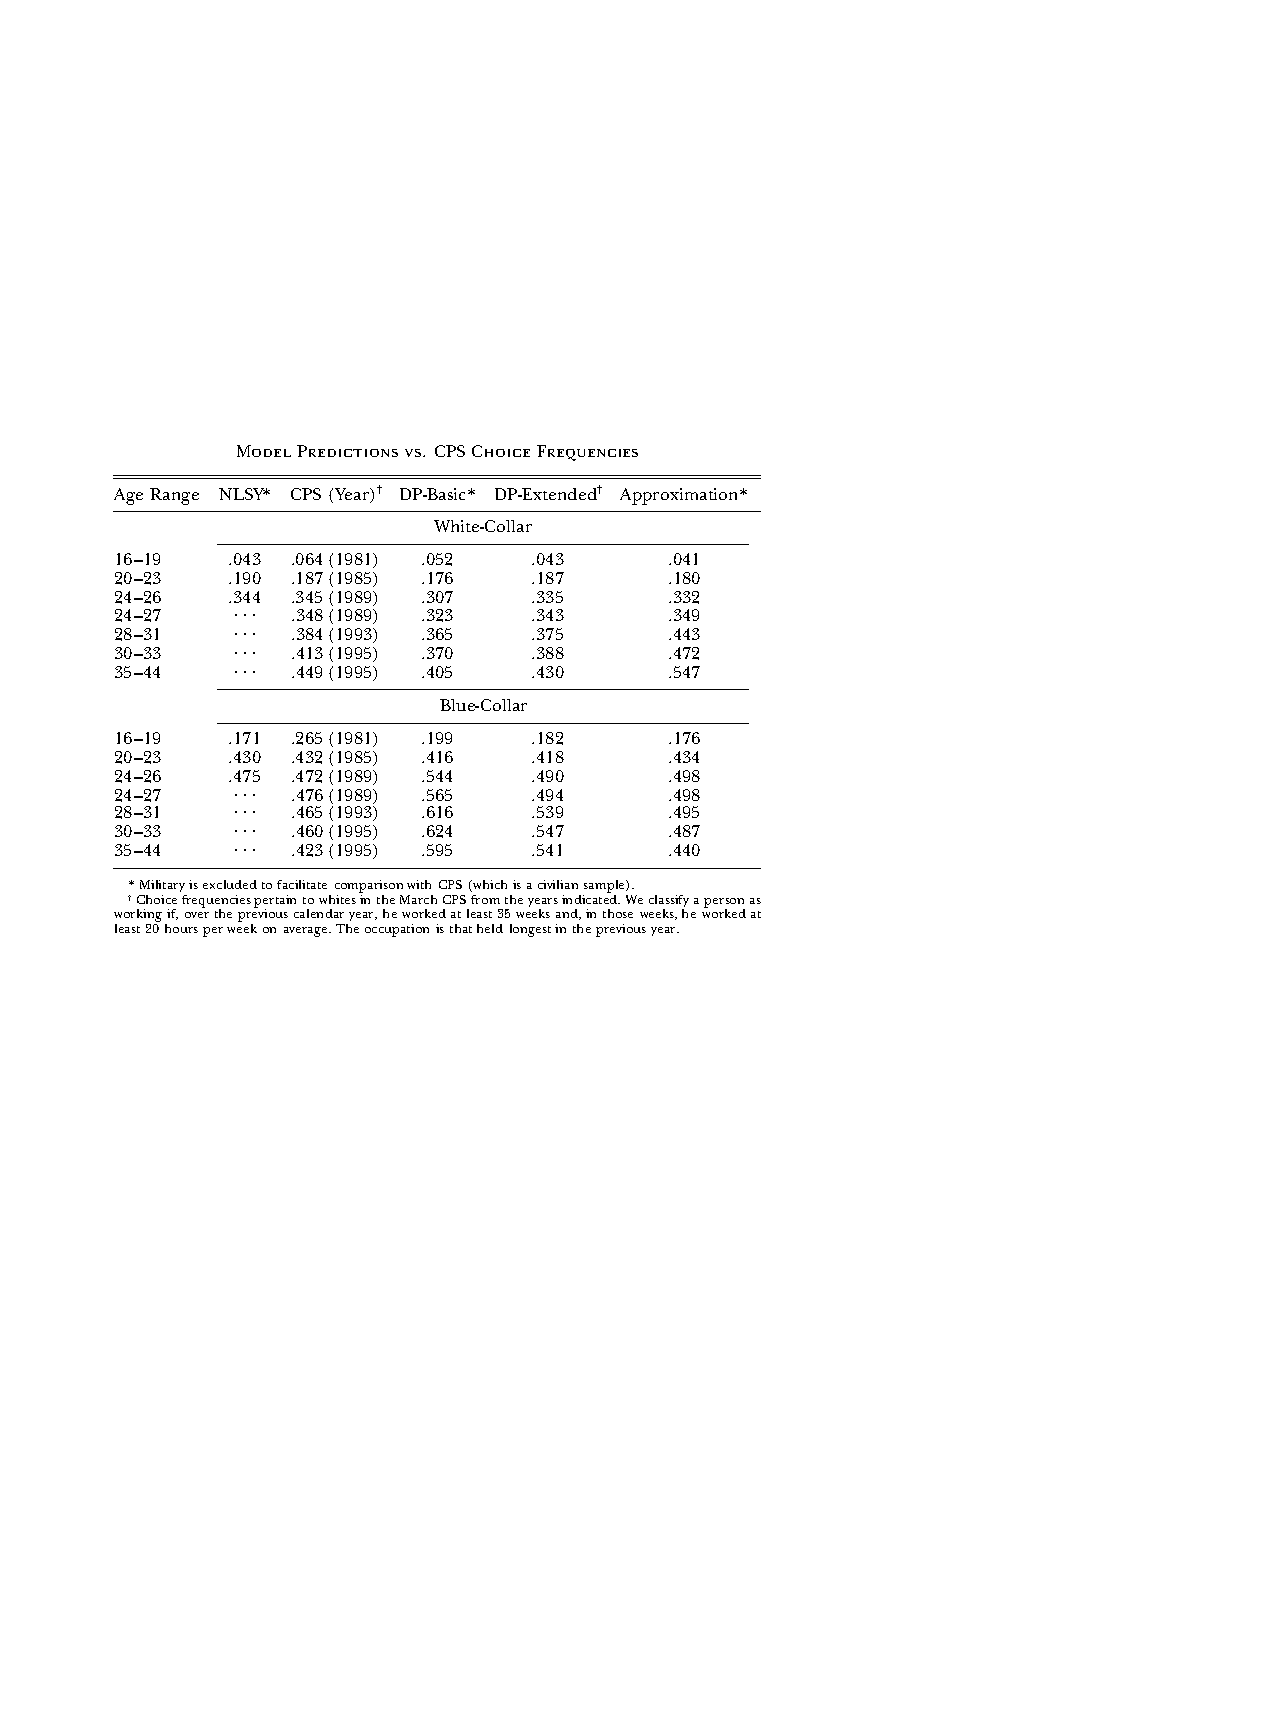
\includegraphics[width=.9\textwidth]{tab-figs/table10_1997}
	\end{center}
\end{frame}

\section{Results}
\begin{frame}
	\frametitle{Behavior by Type: Females}
	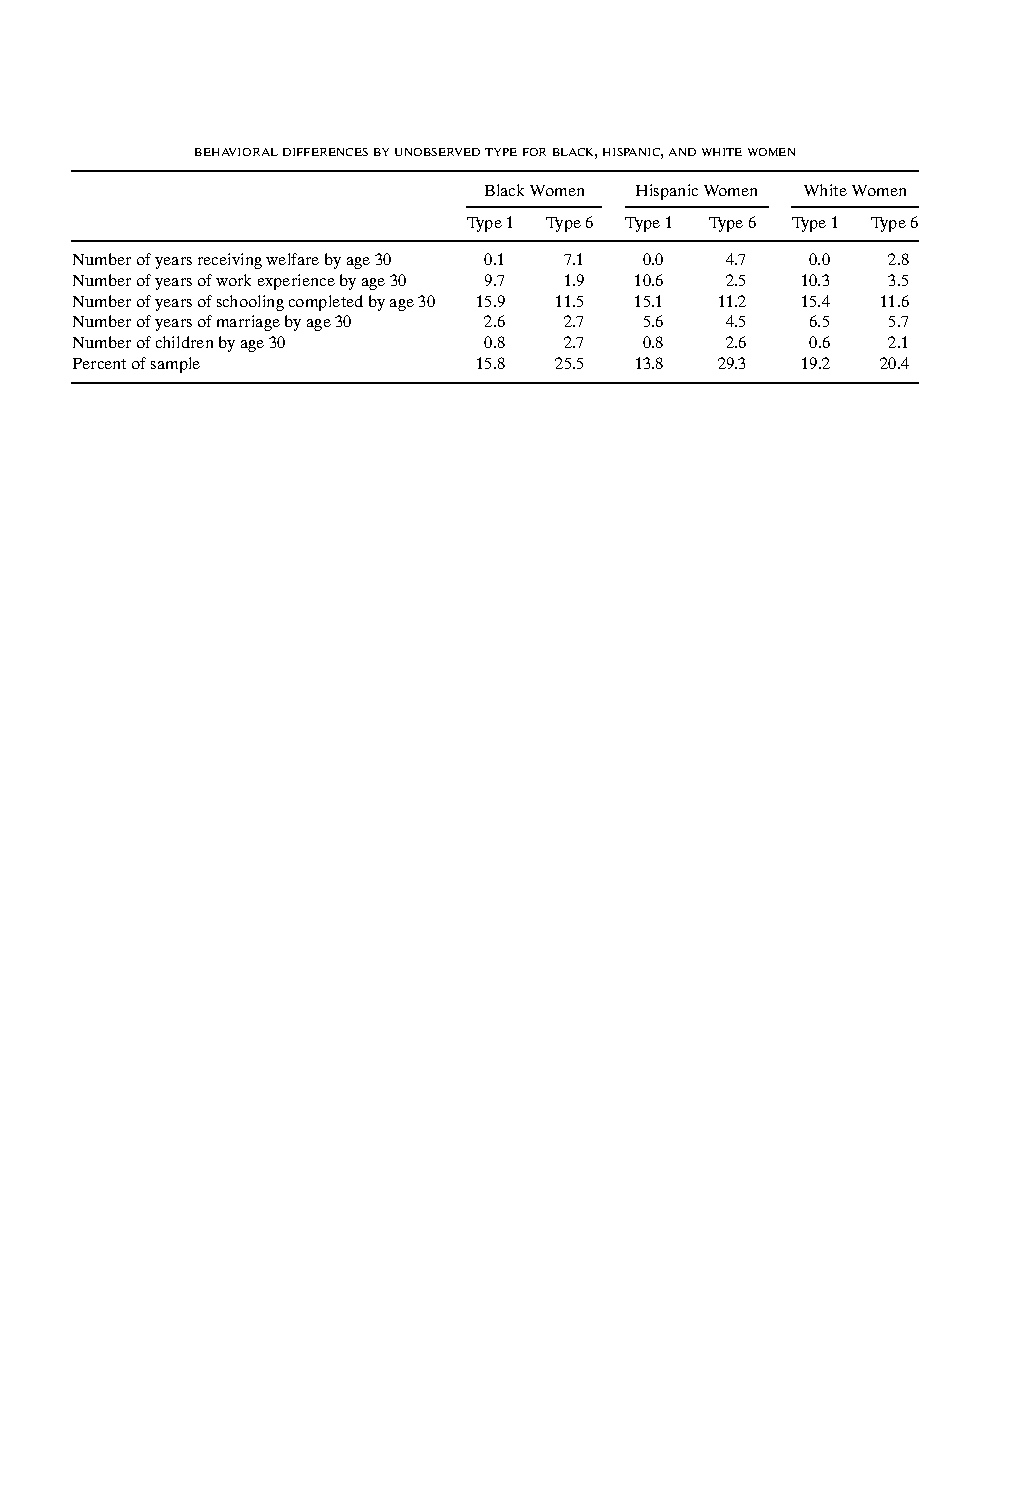
\includegraphics[width=\textwidth]{tab-figs/table3_2010}	
\end{frame}

\begin{frame}
	\frametitle{Variance Explained by Initial Conditions: Females}
	
\includegraphics[width=\textwidth]{tab-figs/table4_2010_header} \\
	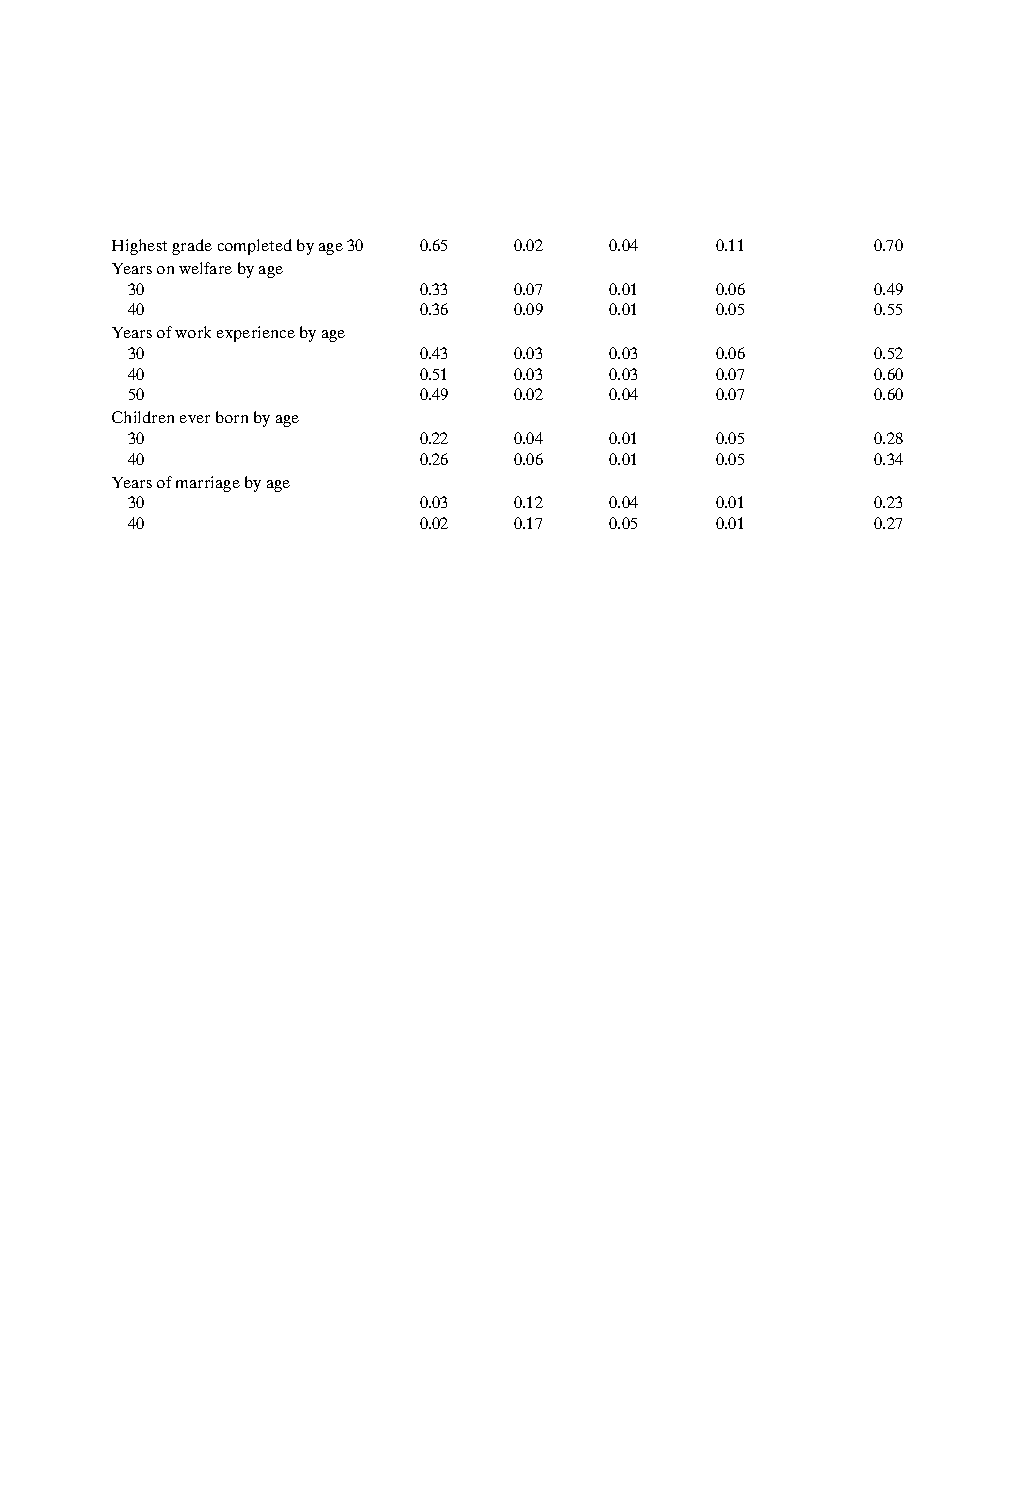
\includegraphics[width=\textwidth]{tab-figs/table4a_2010} \\
	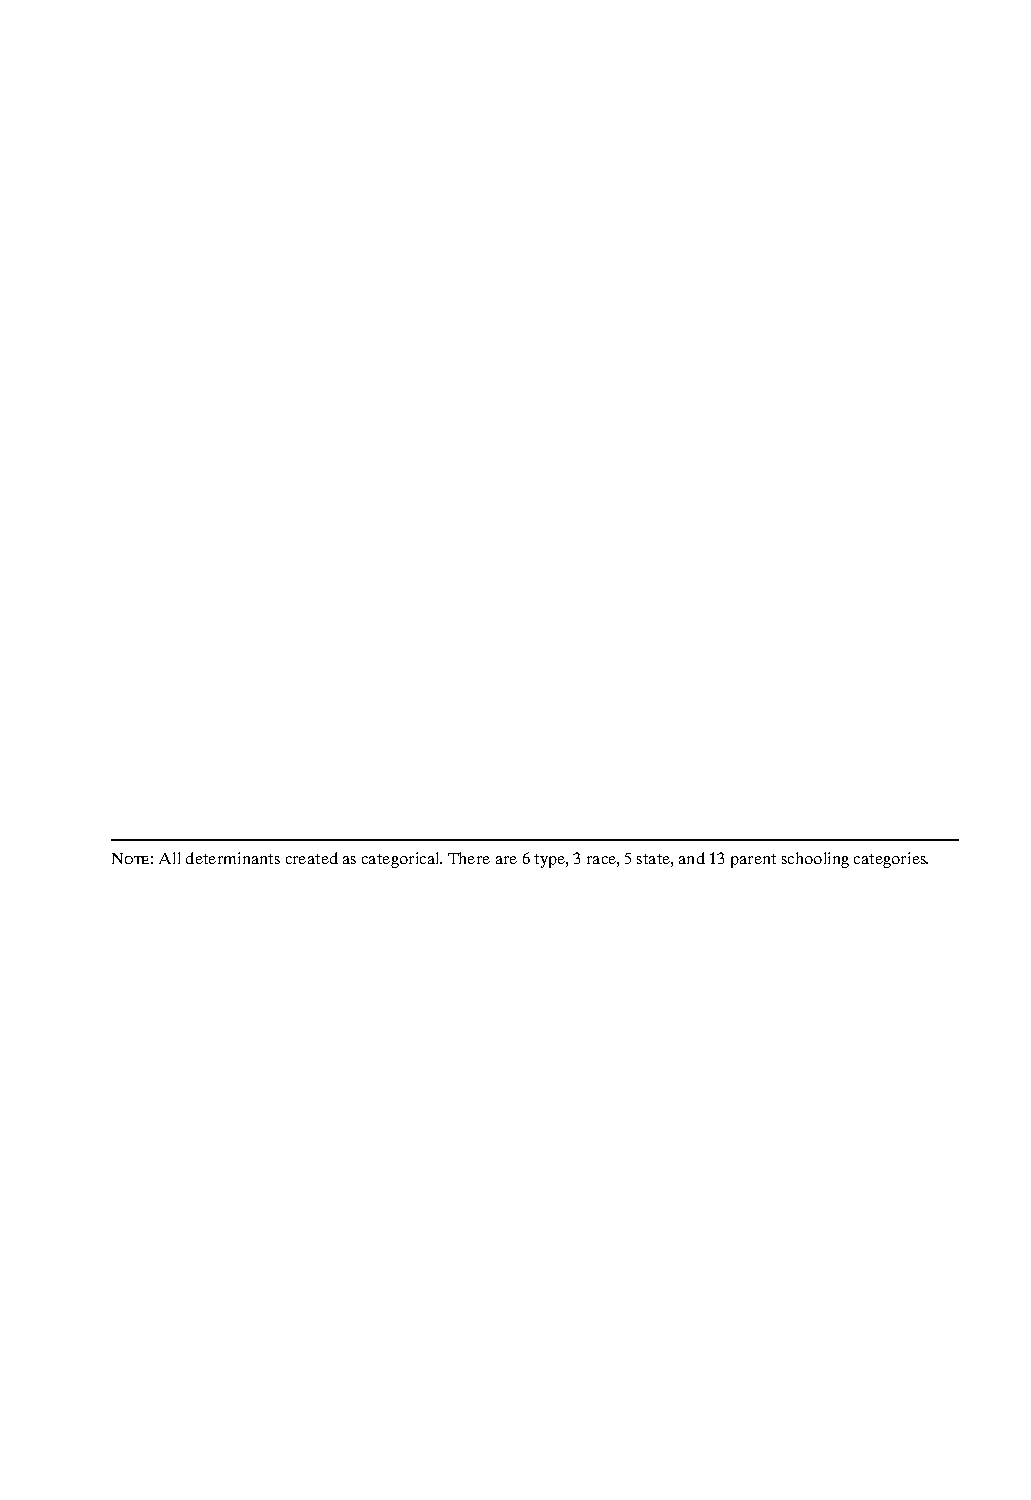
\includegraphics[width=\textwidth]{tab-figs/table4_2010_footer}
\end{frame}

\begin{frame}
	\frametitle{\begin{small}Variance Explained by Initial Conditions (contd): Females\end{small}}
	
\includegraphics[width=\textwidth]{tab-figs/table4_2010_header} \\
	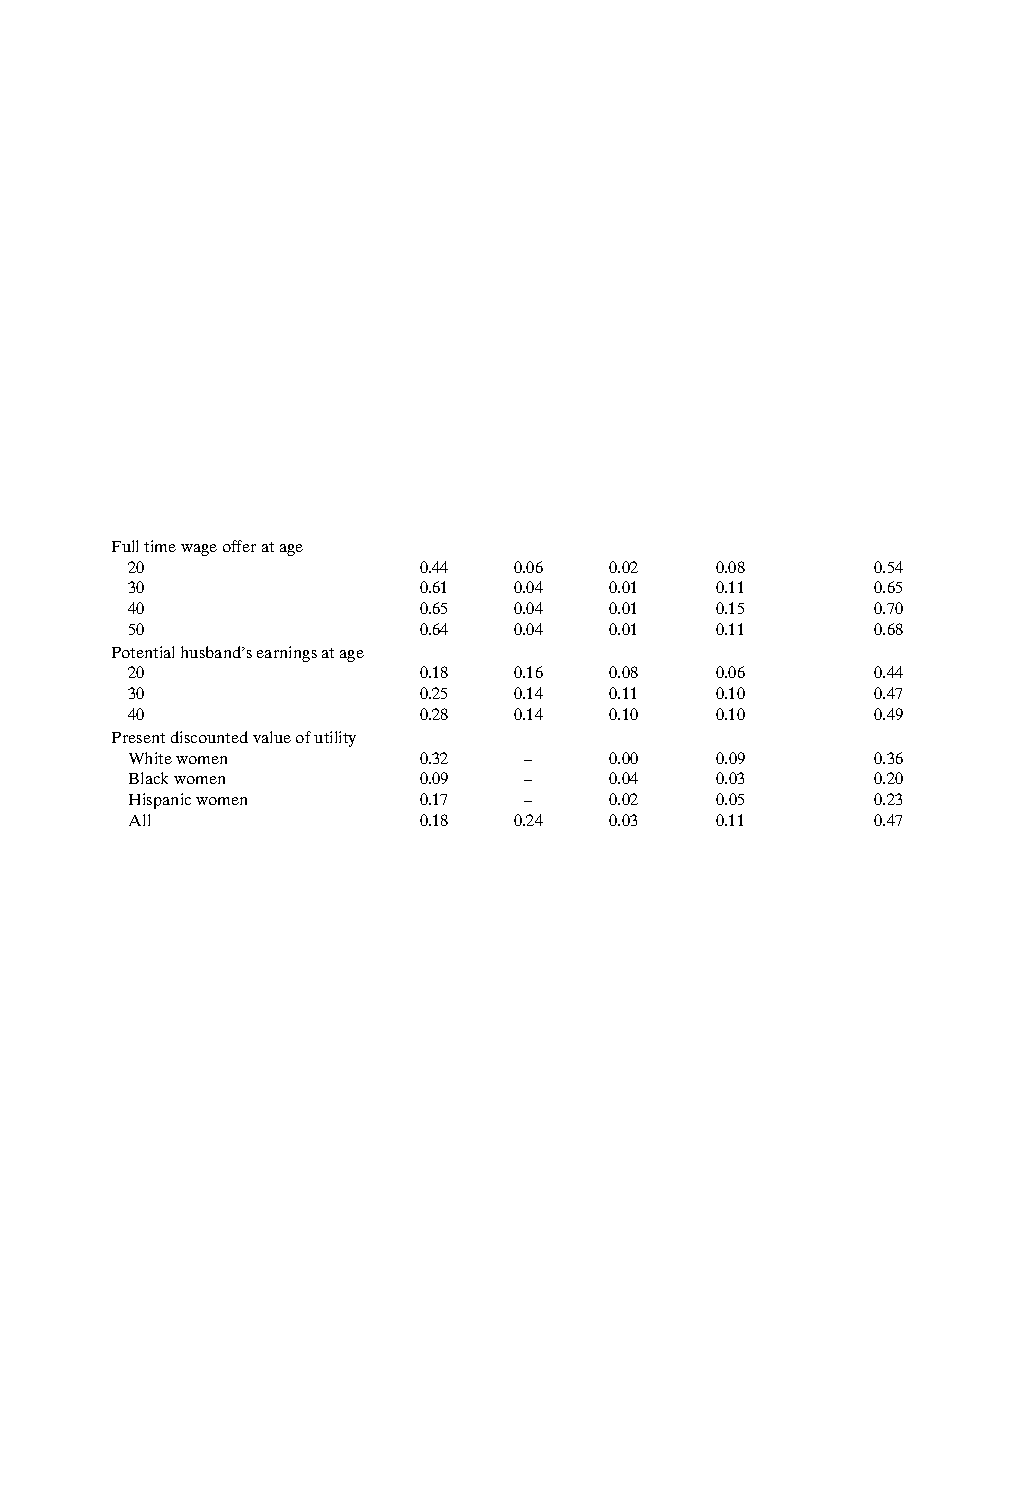
\includegraphics[width=\textwidth]{tab-figs/table4b_2010} \\
	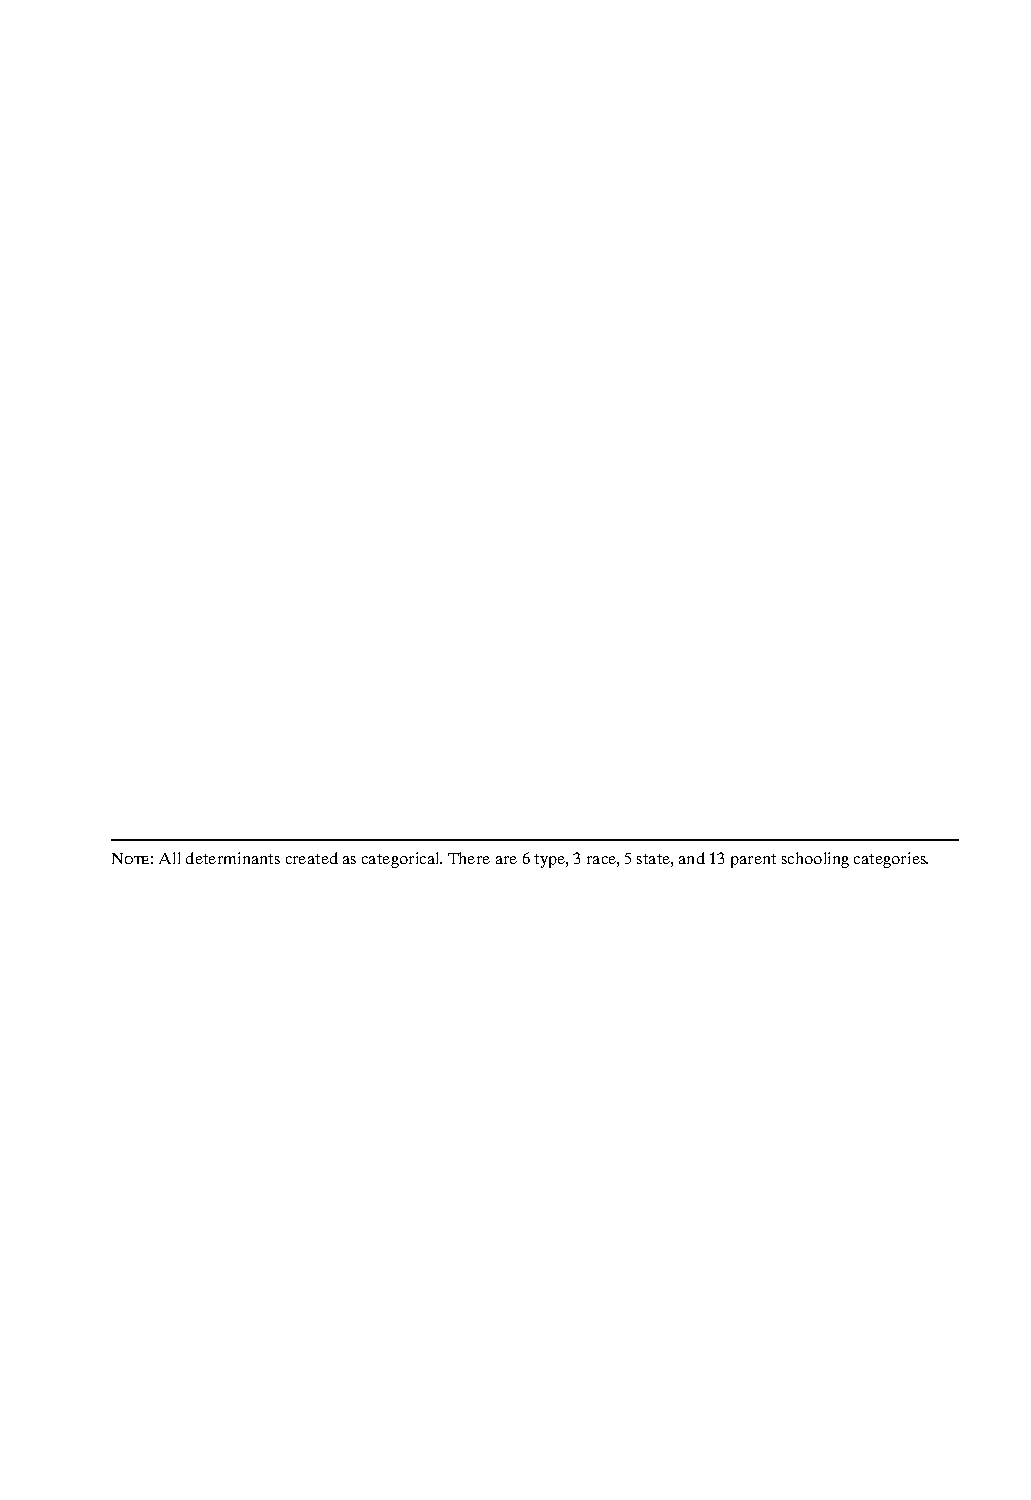
\includegraphics[width=\textwidth]{tab-figs/table4_2010_footer} \\
\end{frame}

\begin{frame}
	\frametitle{Behavior by Type: Males}
	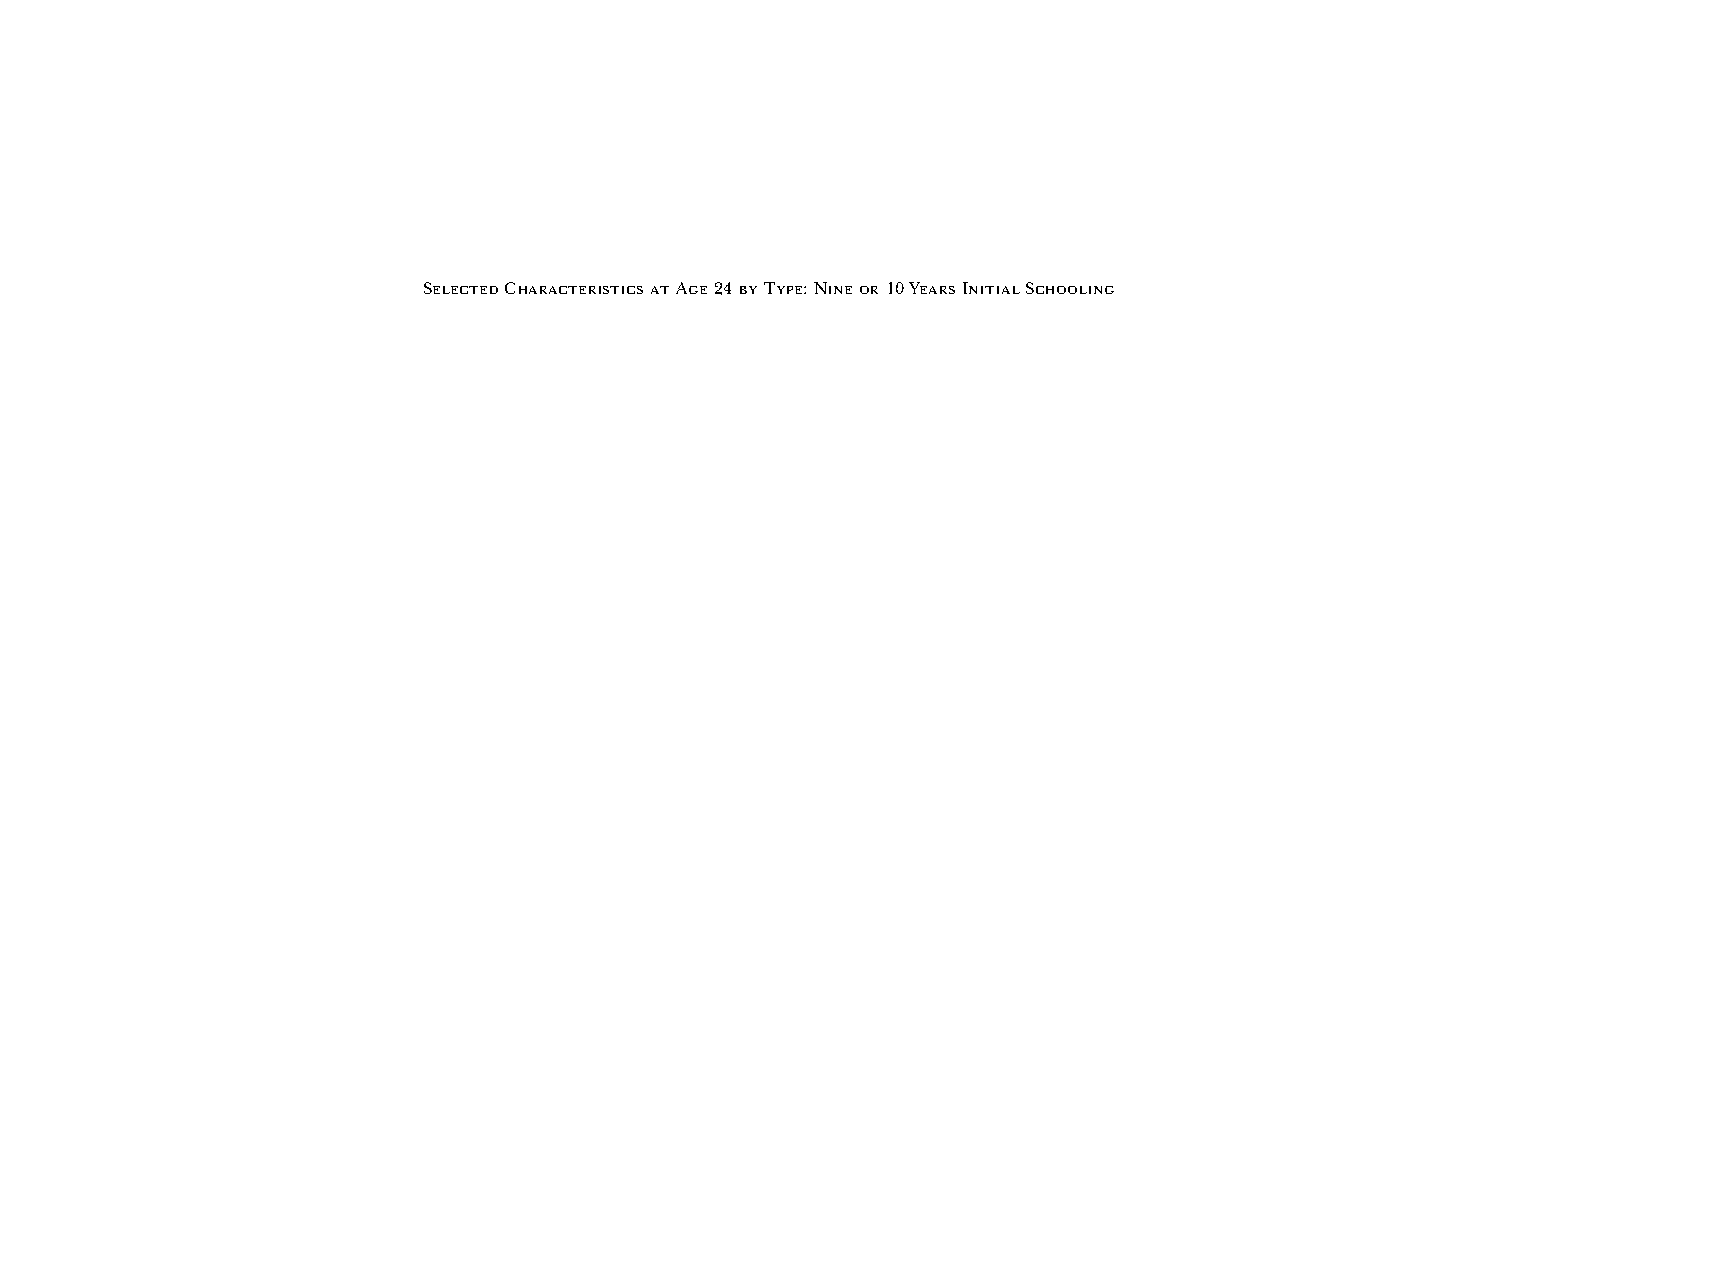
\includegraphics[width=\textwidth]{tab-figs/table11_1997_header}	\\
	
\includegraphics{tab-figs/table11_1997_left}  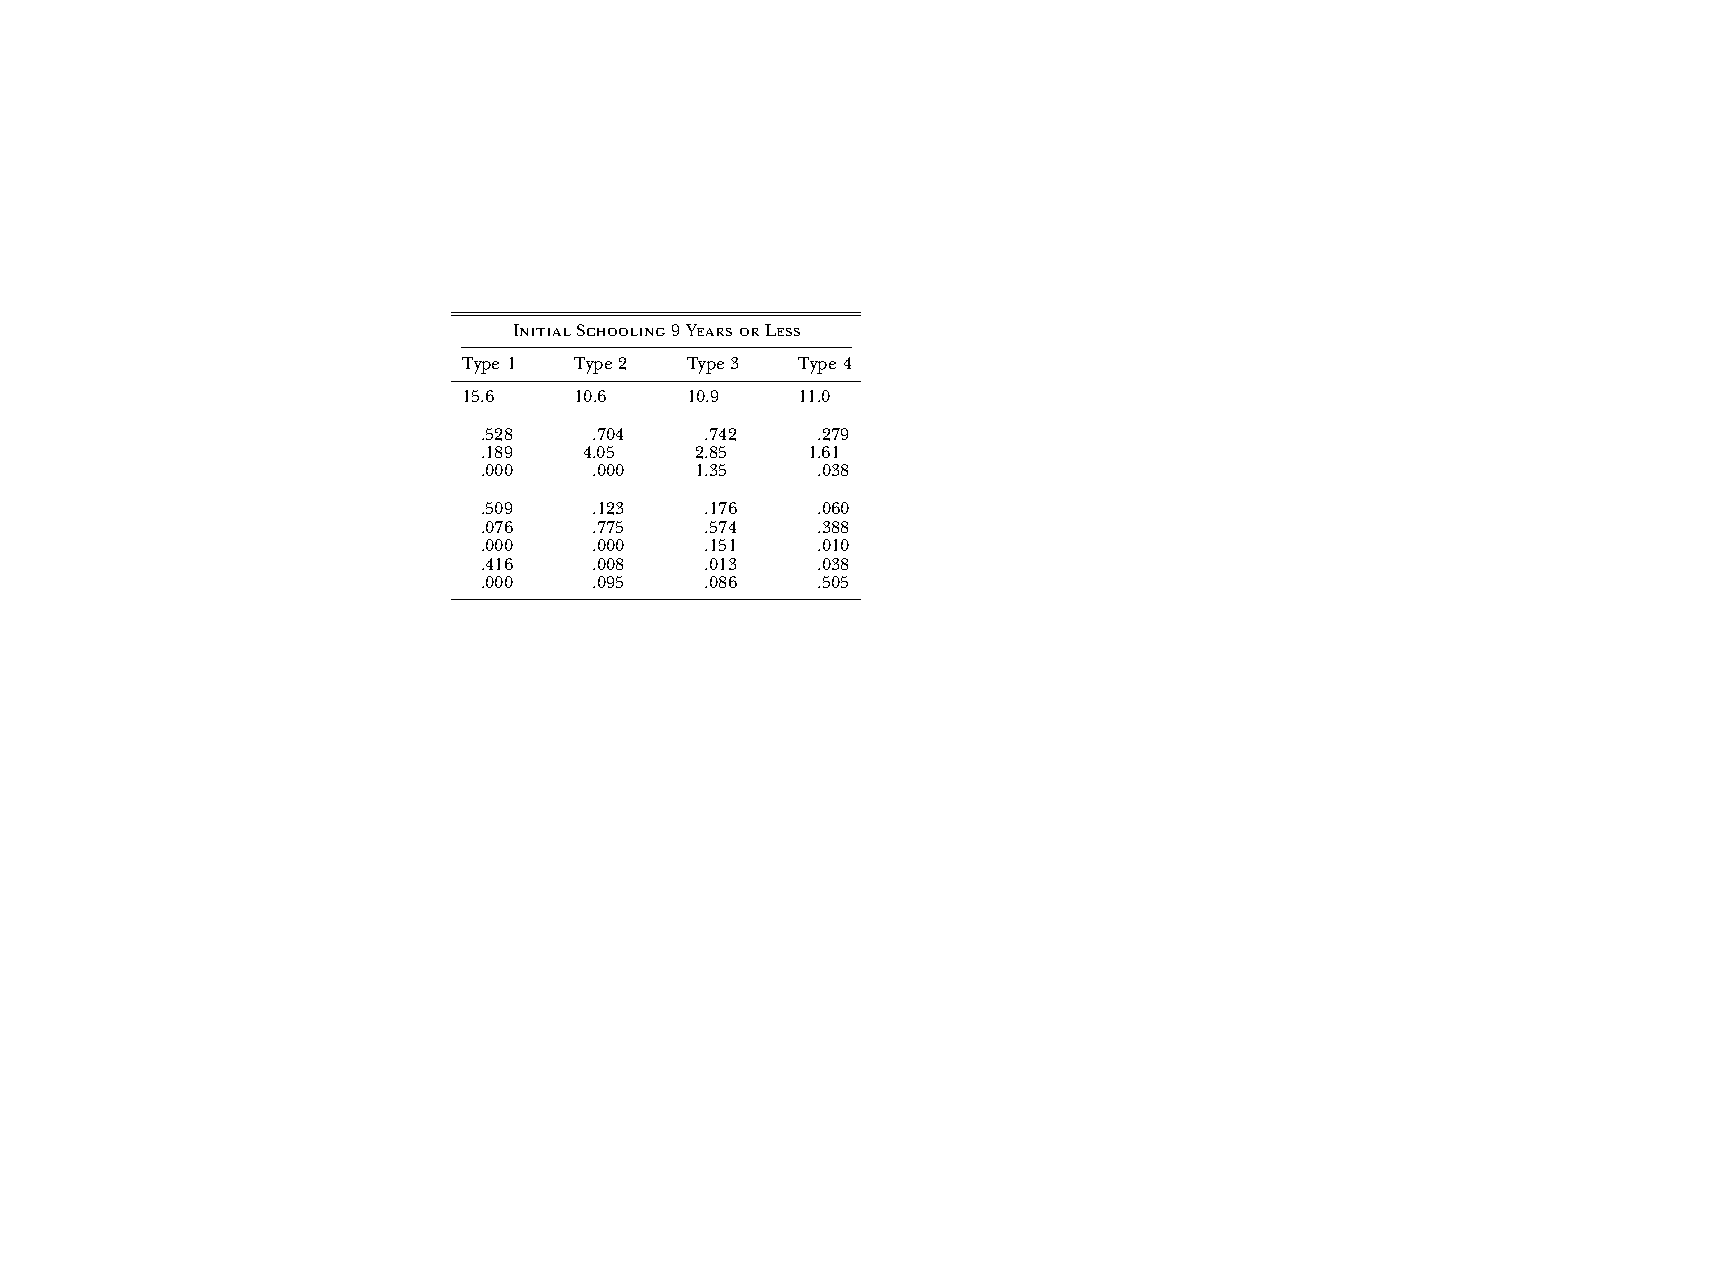
\includegraphics{tab-figs/table11a_1997}	\\	
	
\includegraphics{tab-figs/table11_1997_footer}	
\end{frame}

\begin{frame}
	\frametitle{Behavior by Type (contd): Males}
	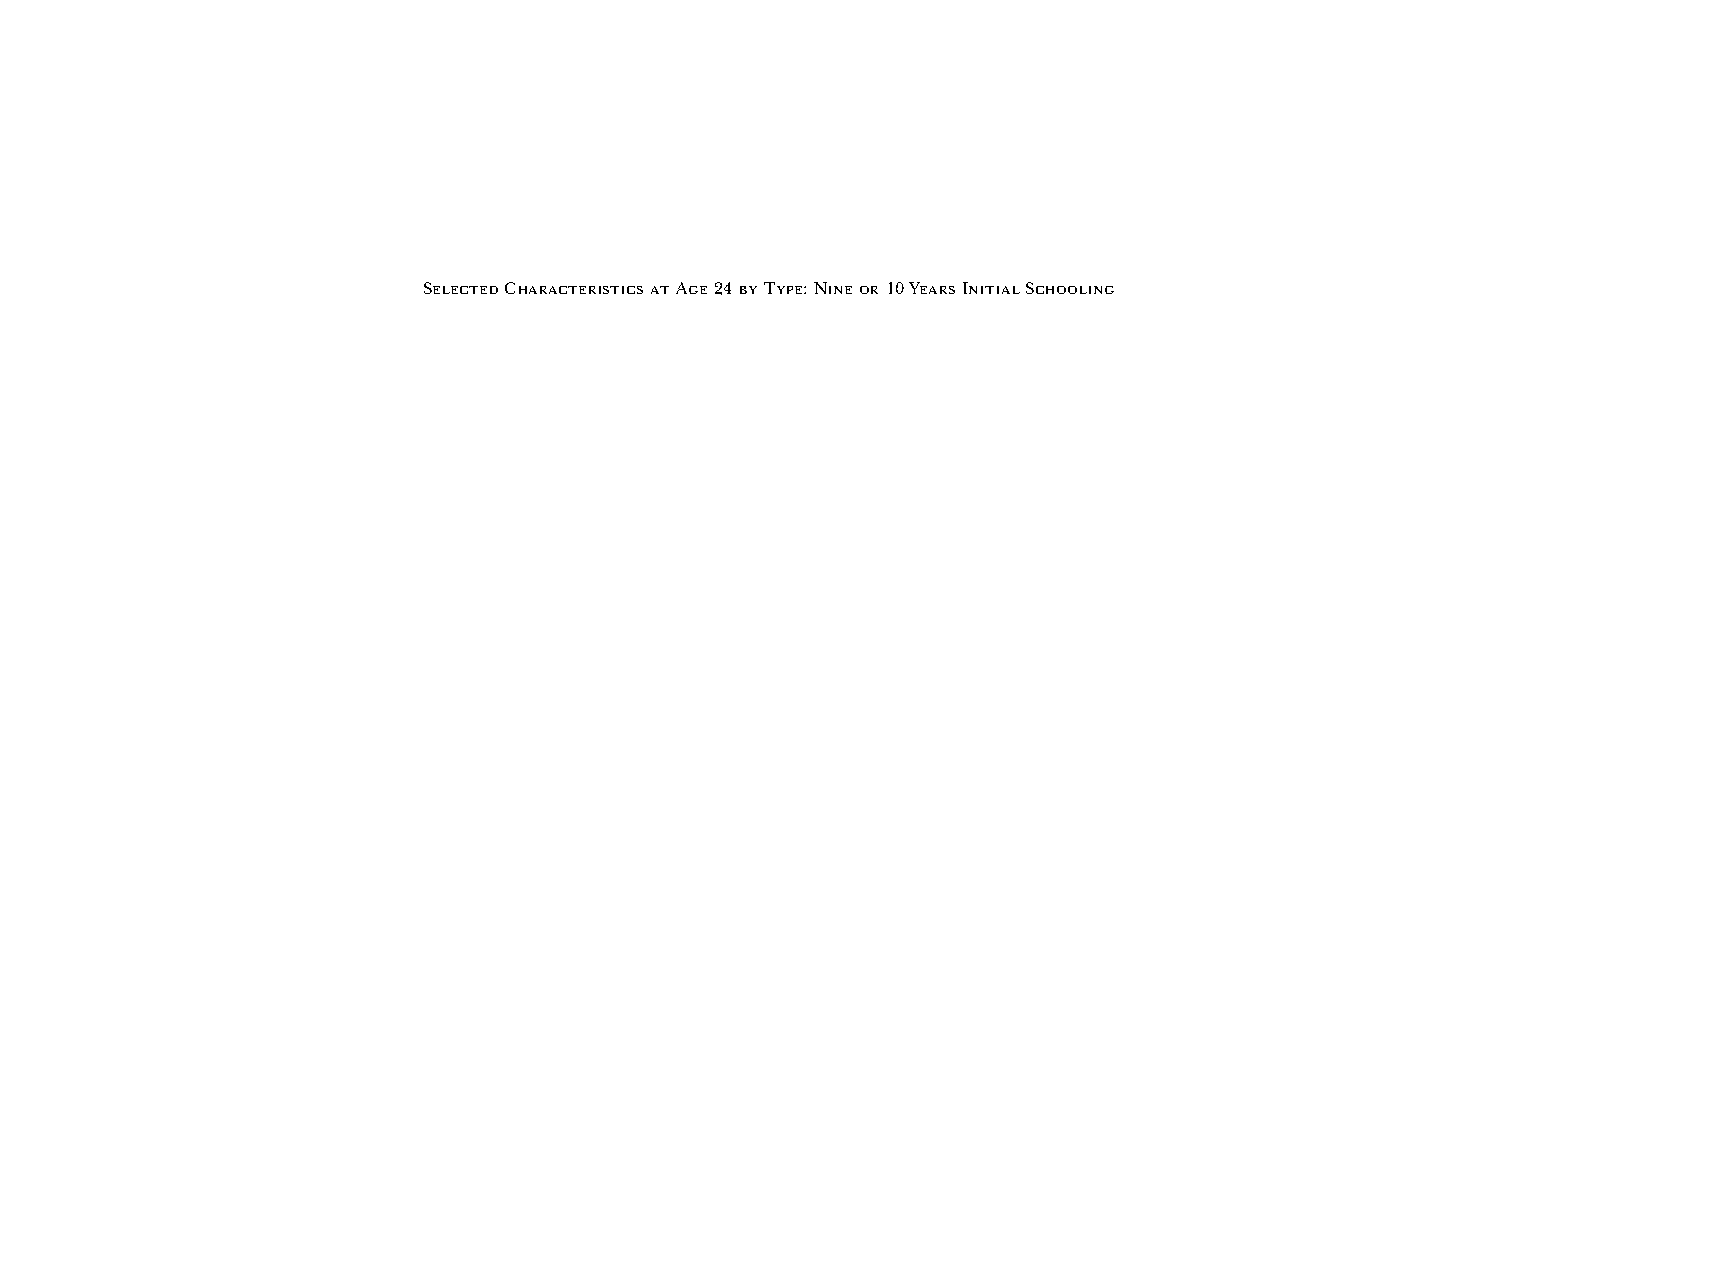
\includegraphics[width=\textwidth]{tab-figs/table11_1997_header}	\\
	
\includegraphics{tab-figs/table11_1997_left}  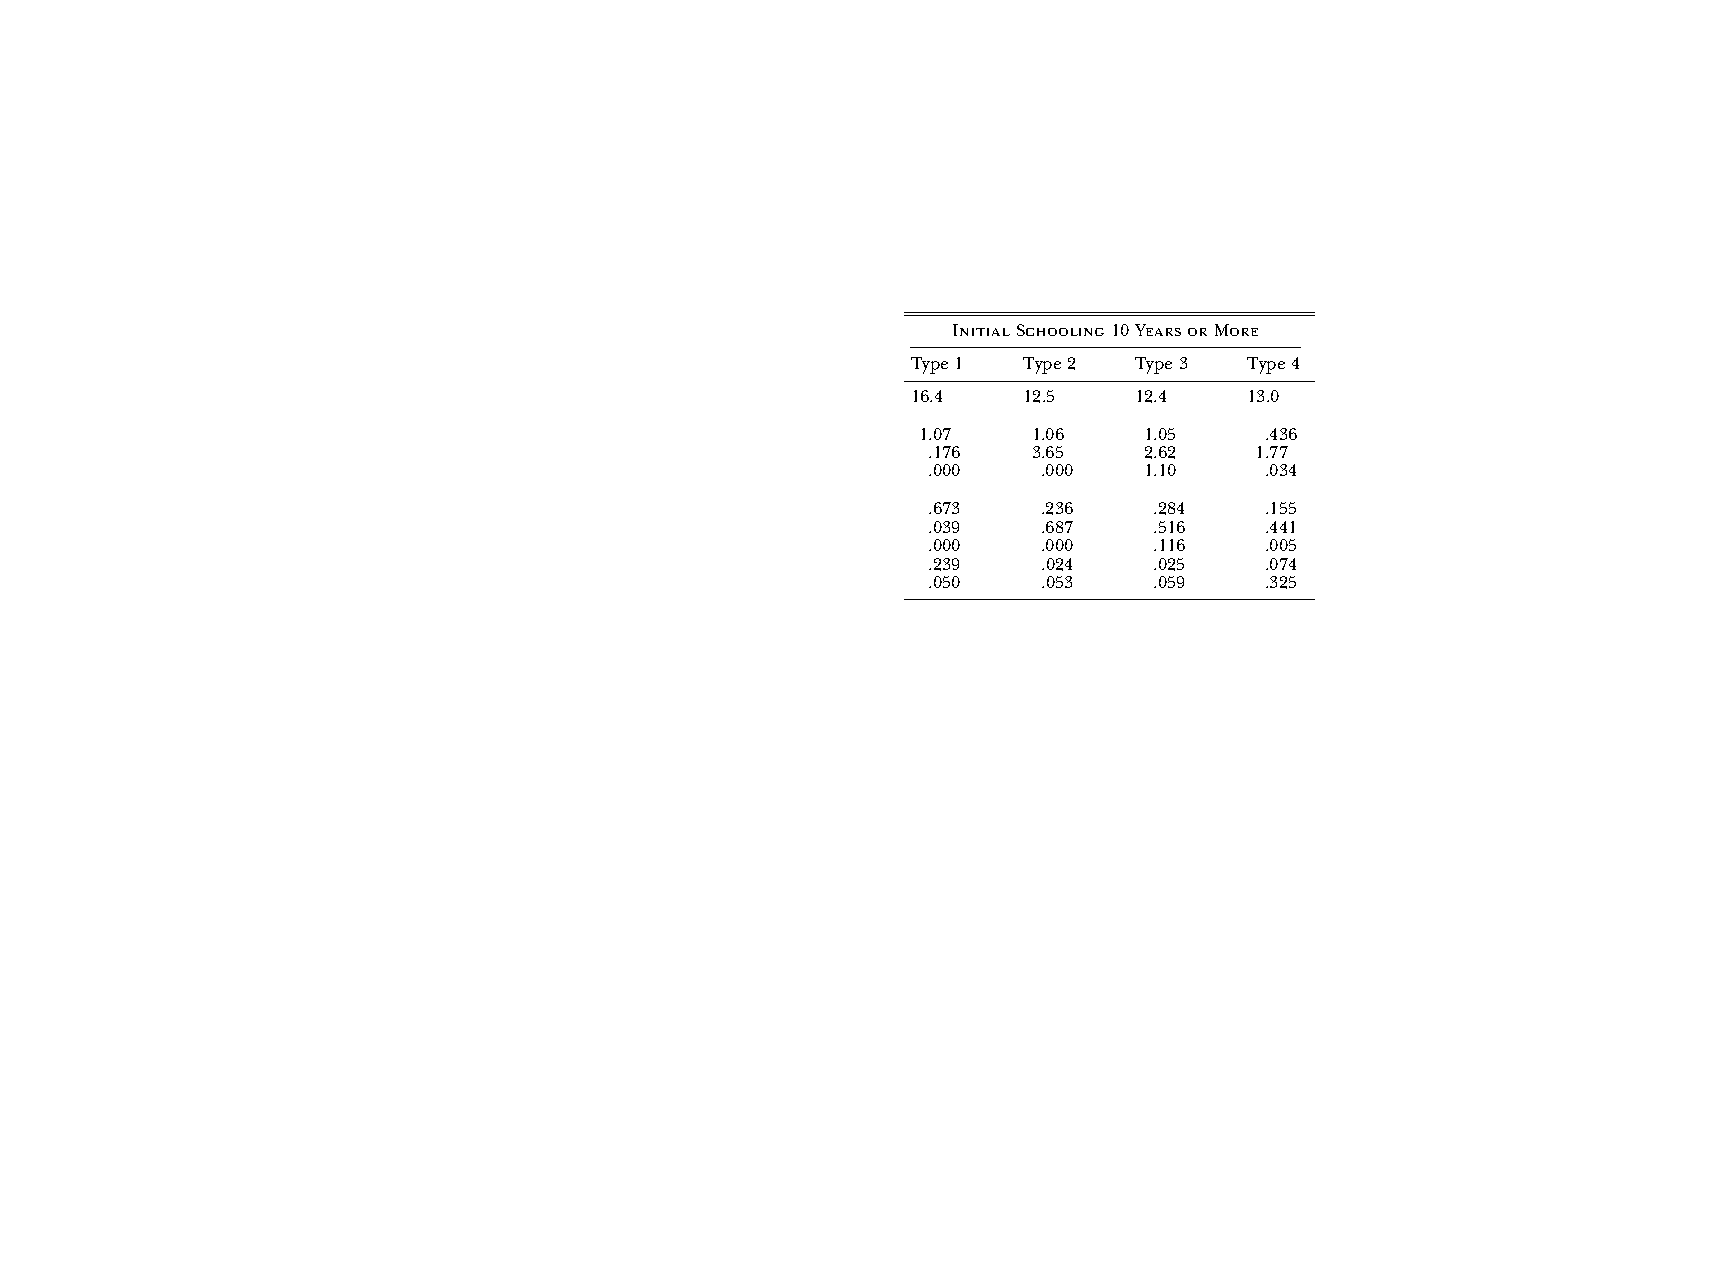
\includegraphics{tab-figs/table11b_1997}	\\	
	
\includegraphics{tab-figs/table11_1997_footer}	
\end{frame}

\begin{frame}
	\frametitle{Type Proportions by Initial Conditions: Males}
	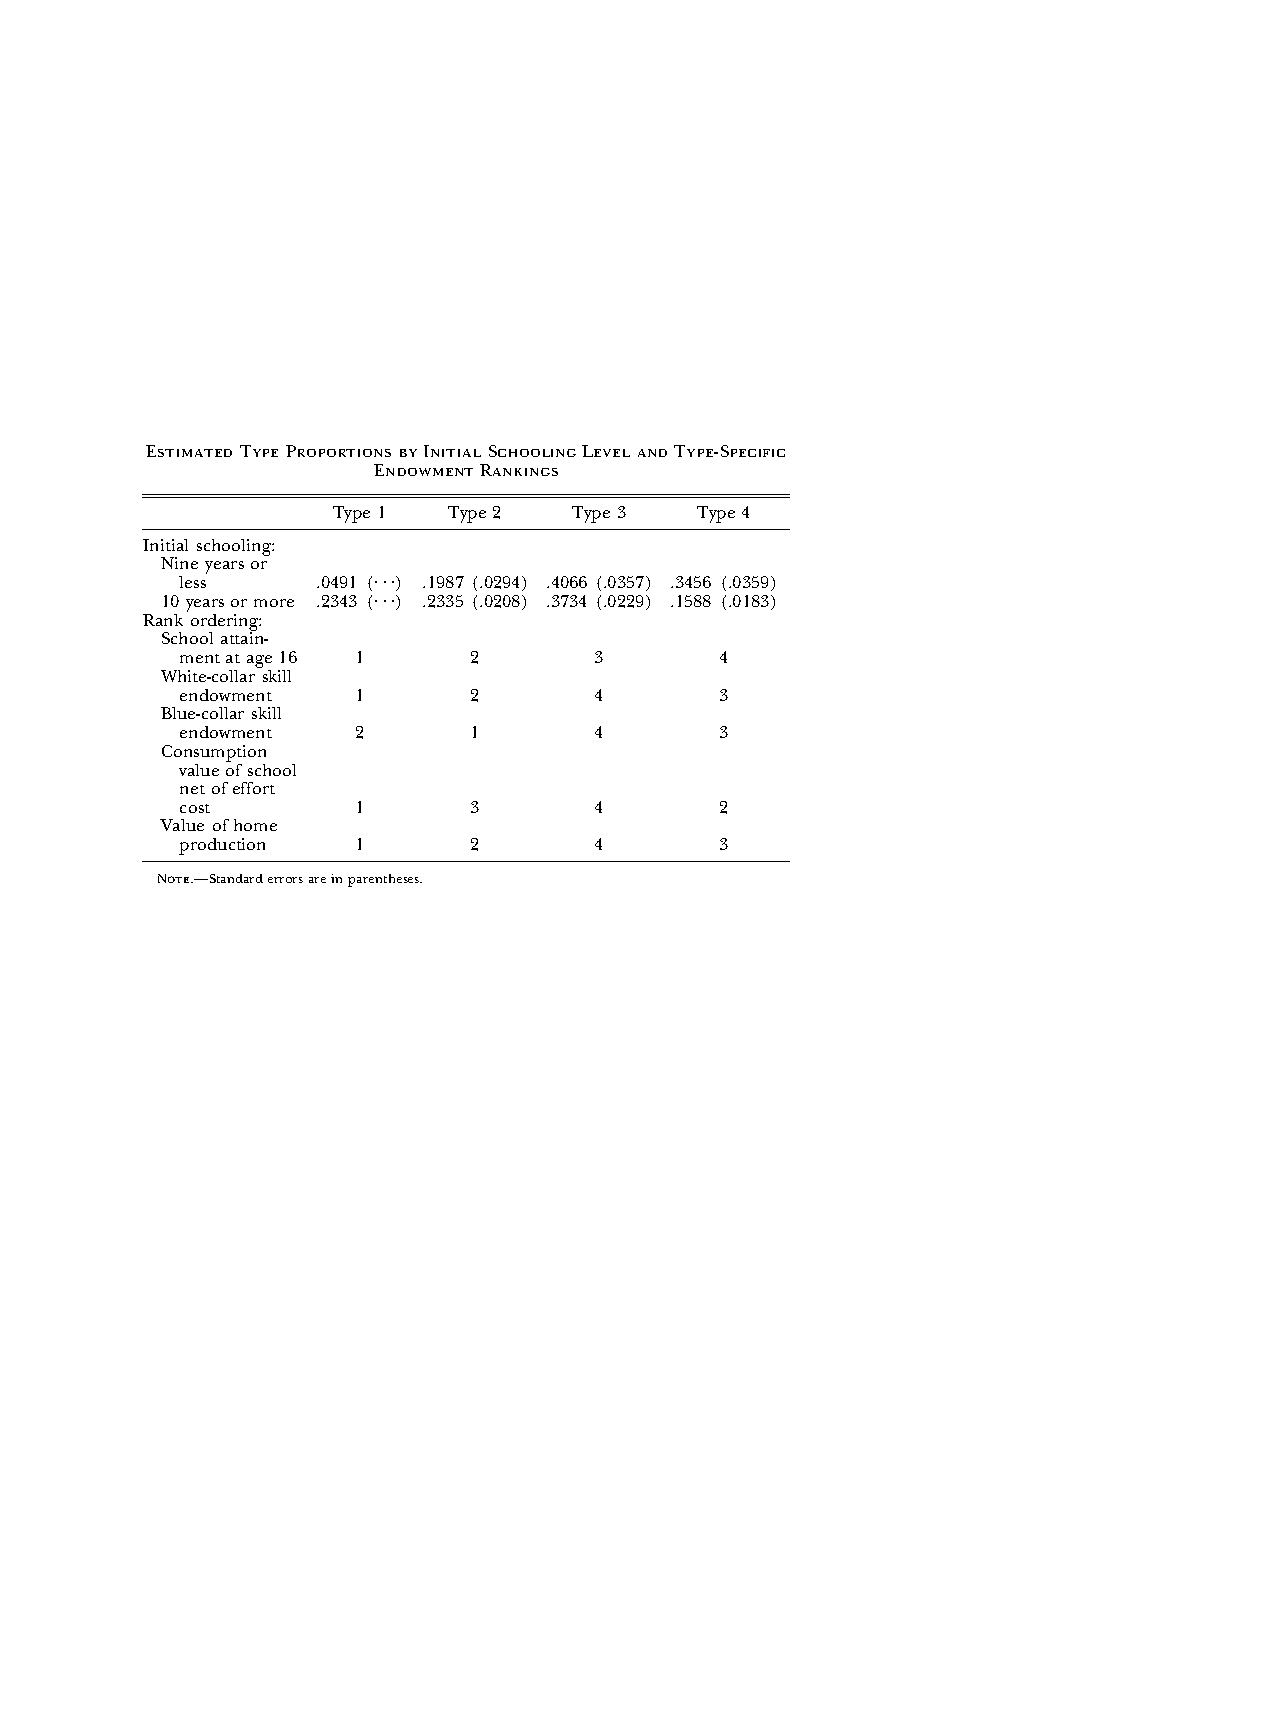
\includegraphics{tab-figs/table9_1997}	
\end{frame}

\begin{frame}
	\frametitle{Family Background: Males}
	
\includegraphics[width=\textwidth]{tab-figs/table13_1997_header}	\\
	\begin{center}
	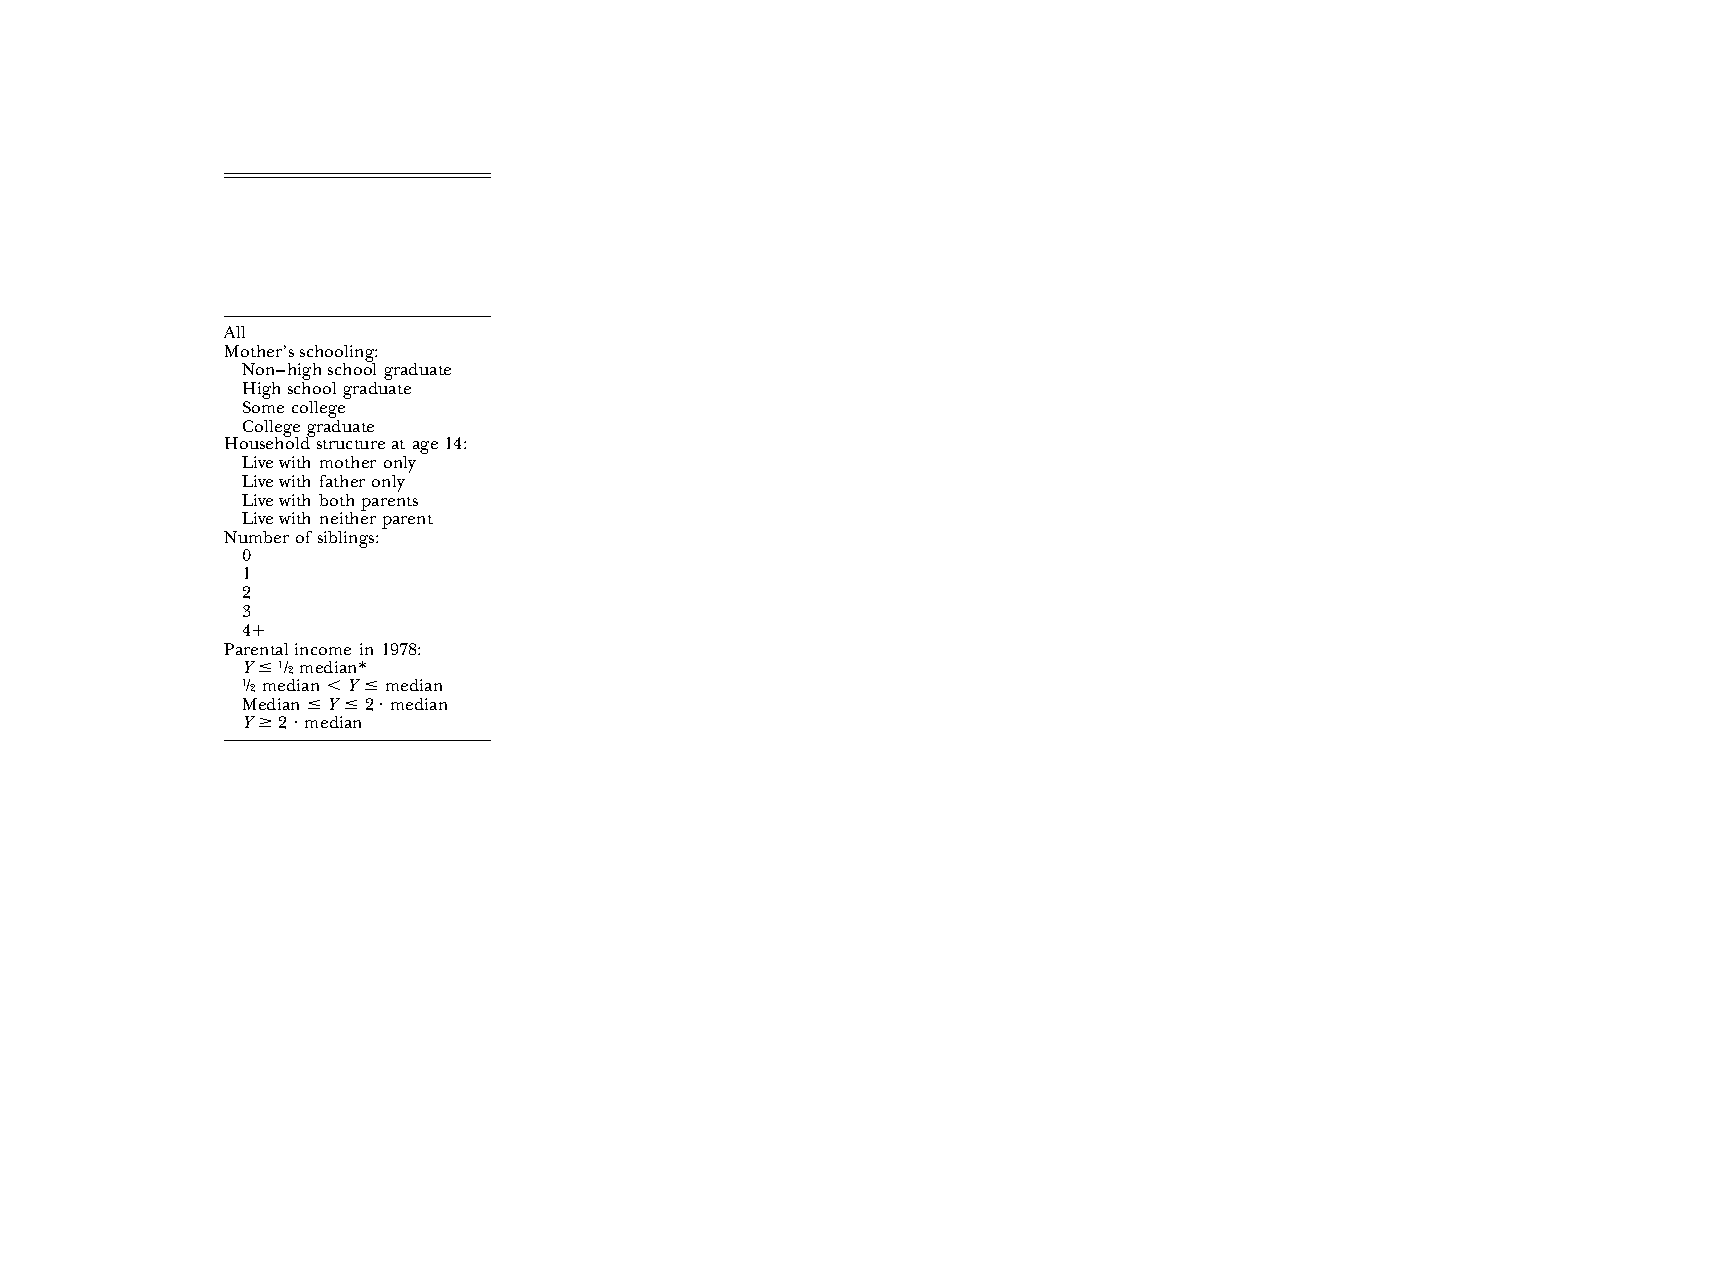
\includegraphics[height=2.75in]{tab-figs/table13_1997_left} 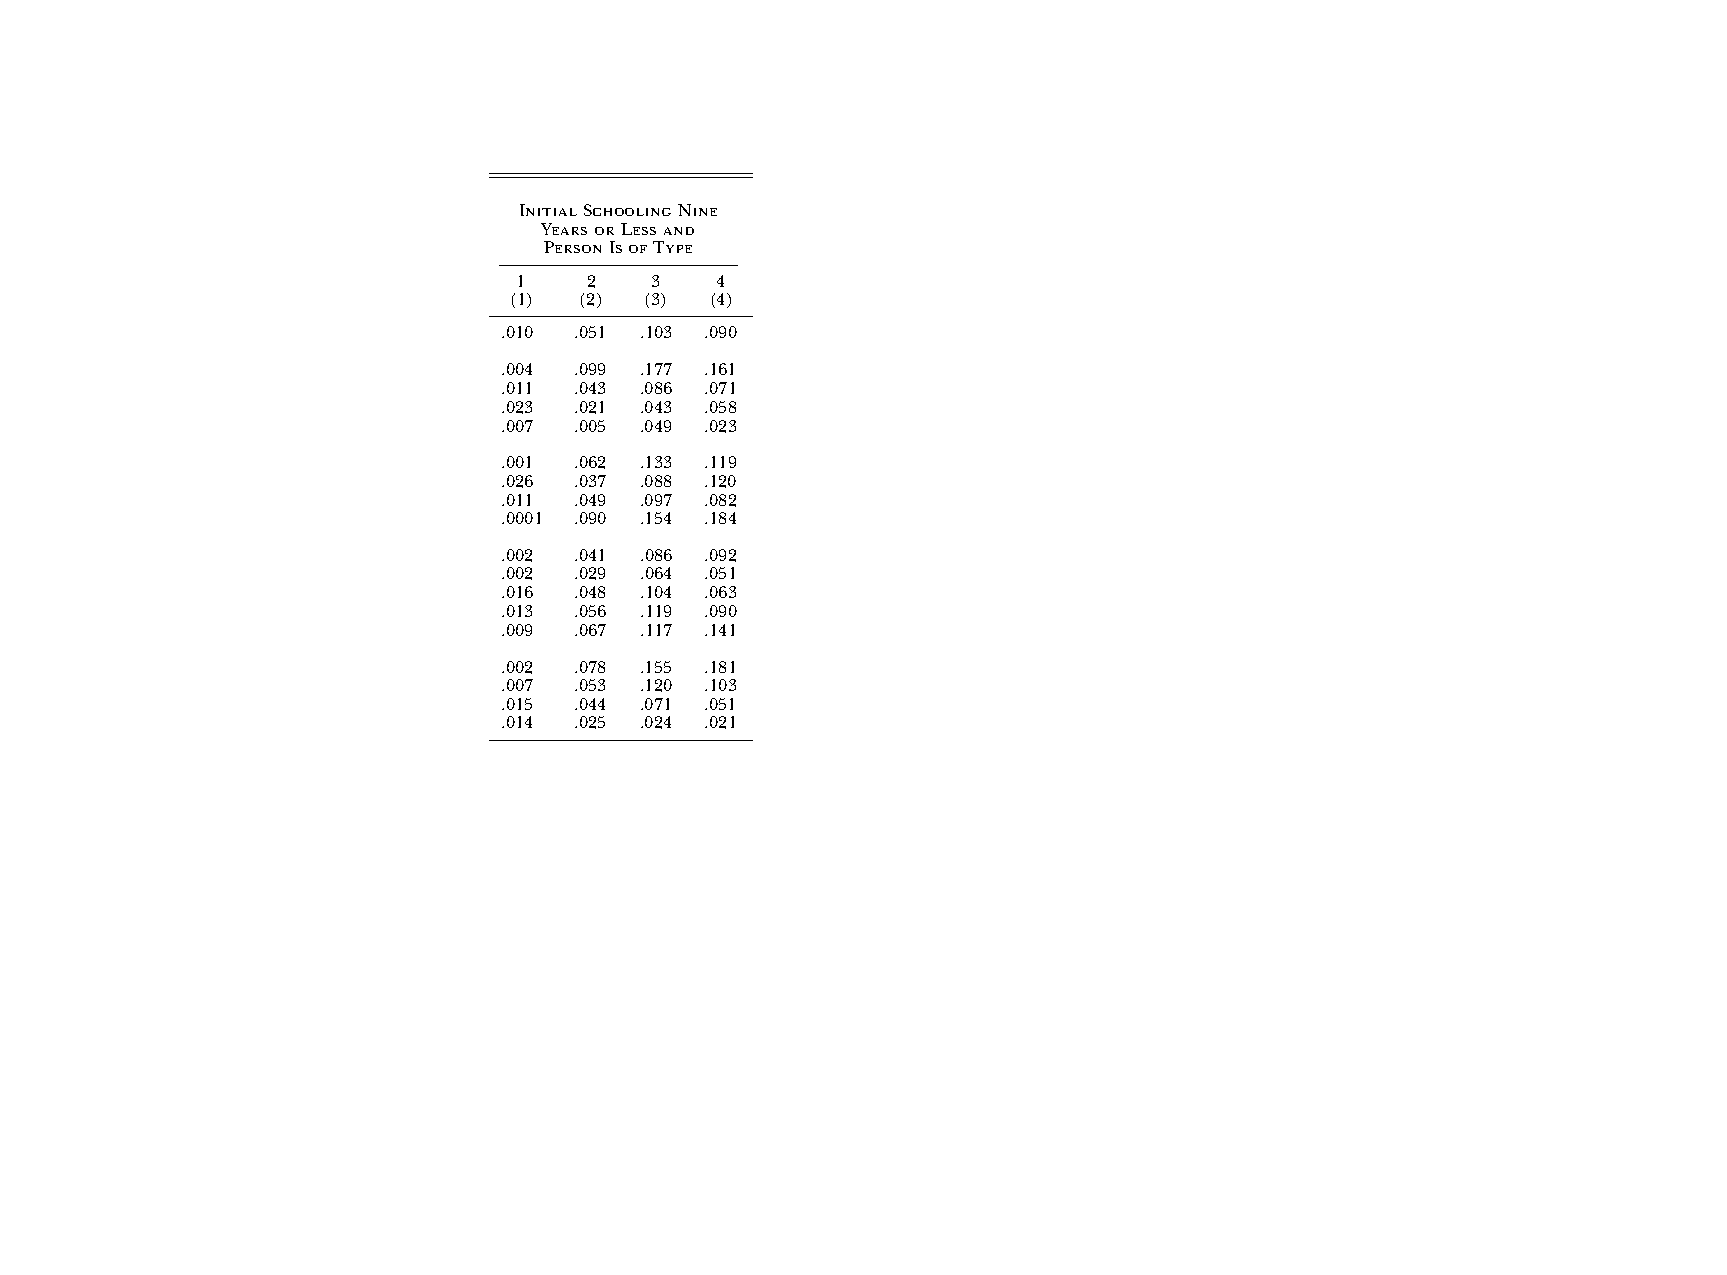
\includegraphics[height=2.75in]{tab-figs/table13a_1997}	\\
	
\includegraphics{tab-figs/table13_1997_footer}	
	\end{center}
\end{frame}

\begin{frame}
	\frametitle{Family Background (contd): Males}
	
\includegraphics[width=\textwidth]{tab-figs/table13_1997_header}	\\
	\begin{center}
	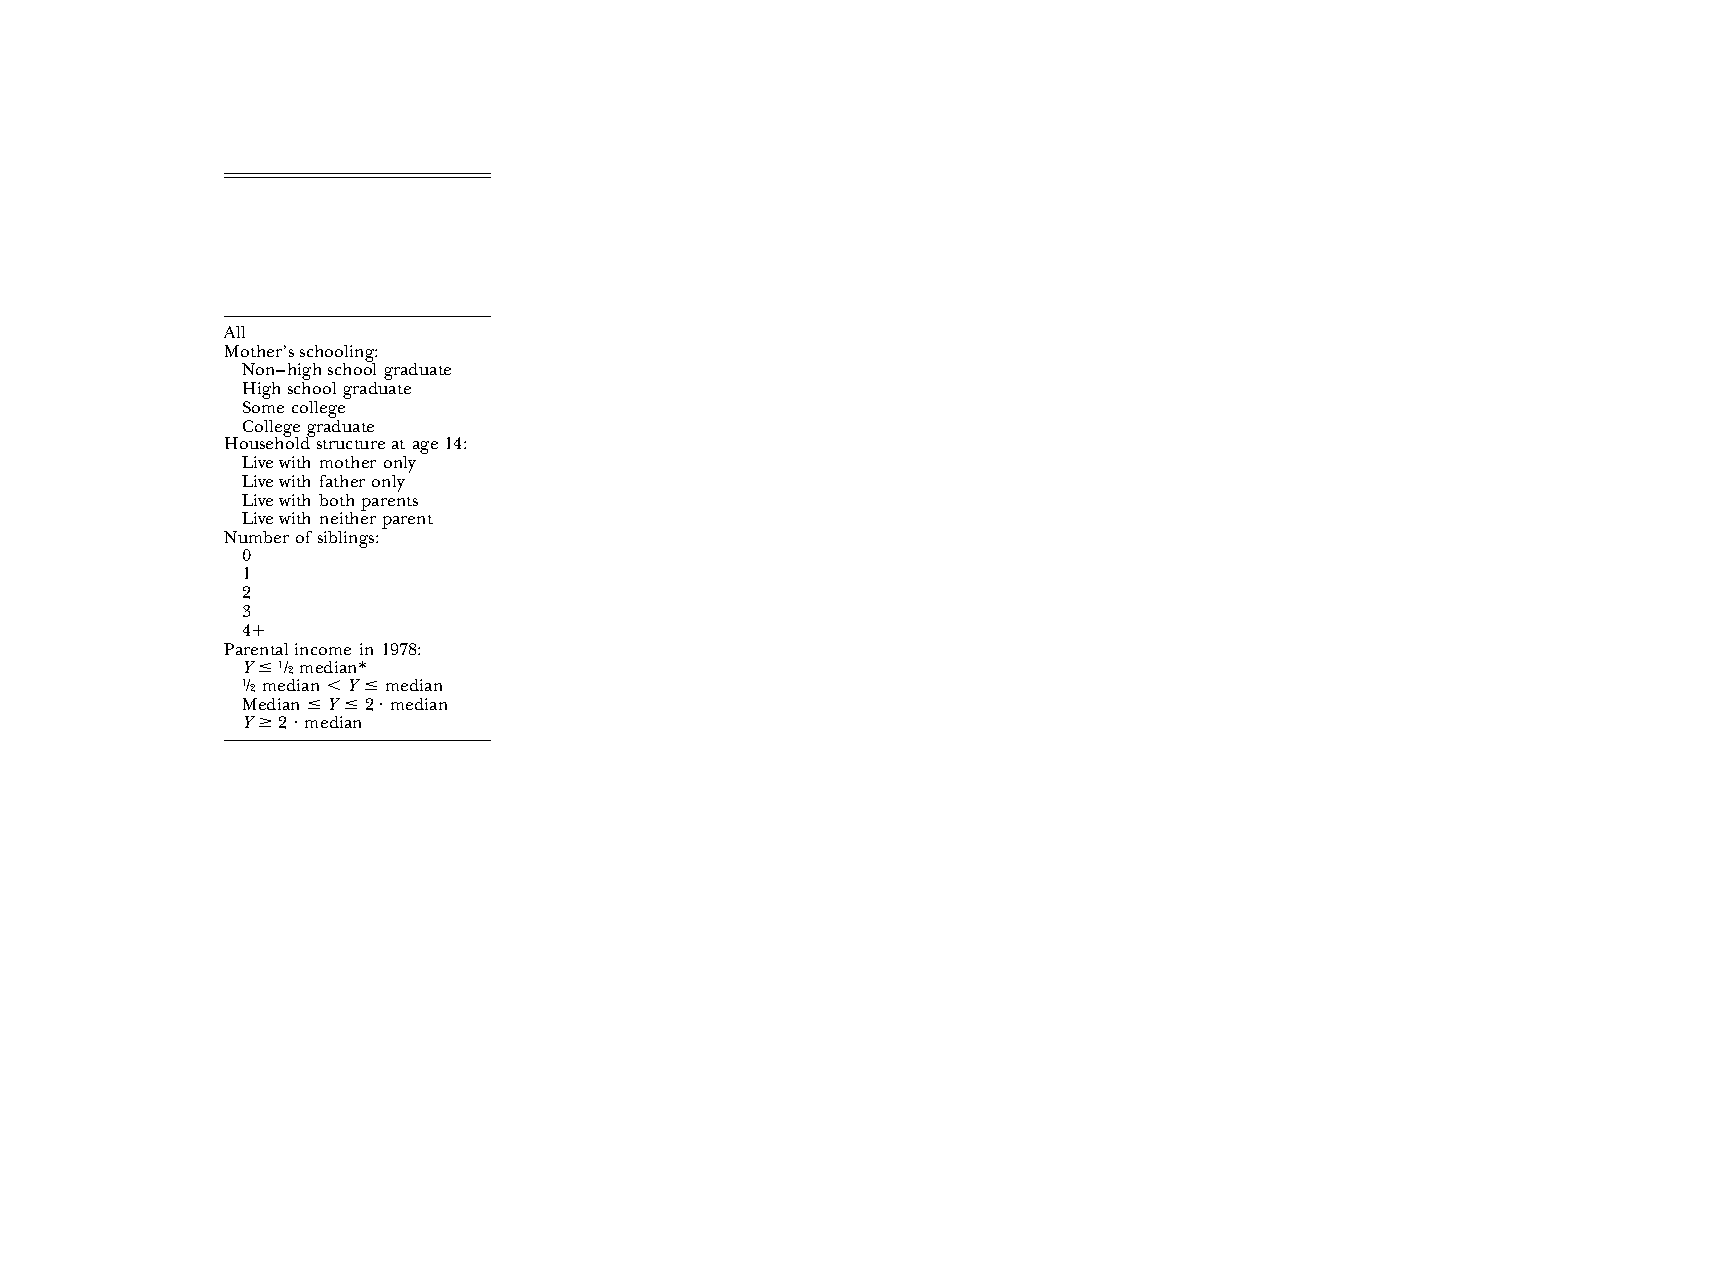
\includegraphics[height=2.75in]{tab-figs/table13_1997_left} 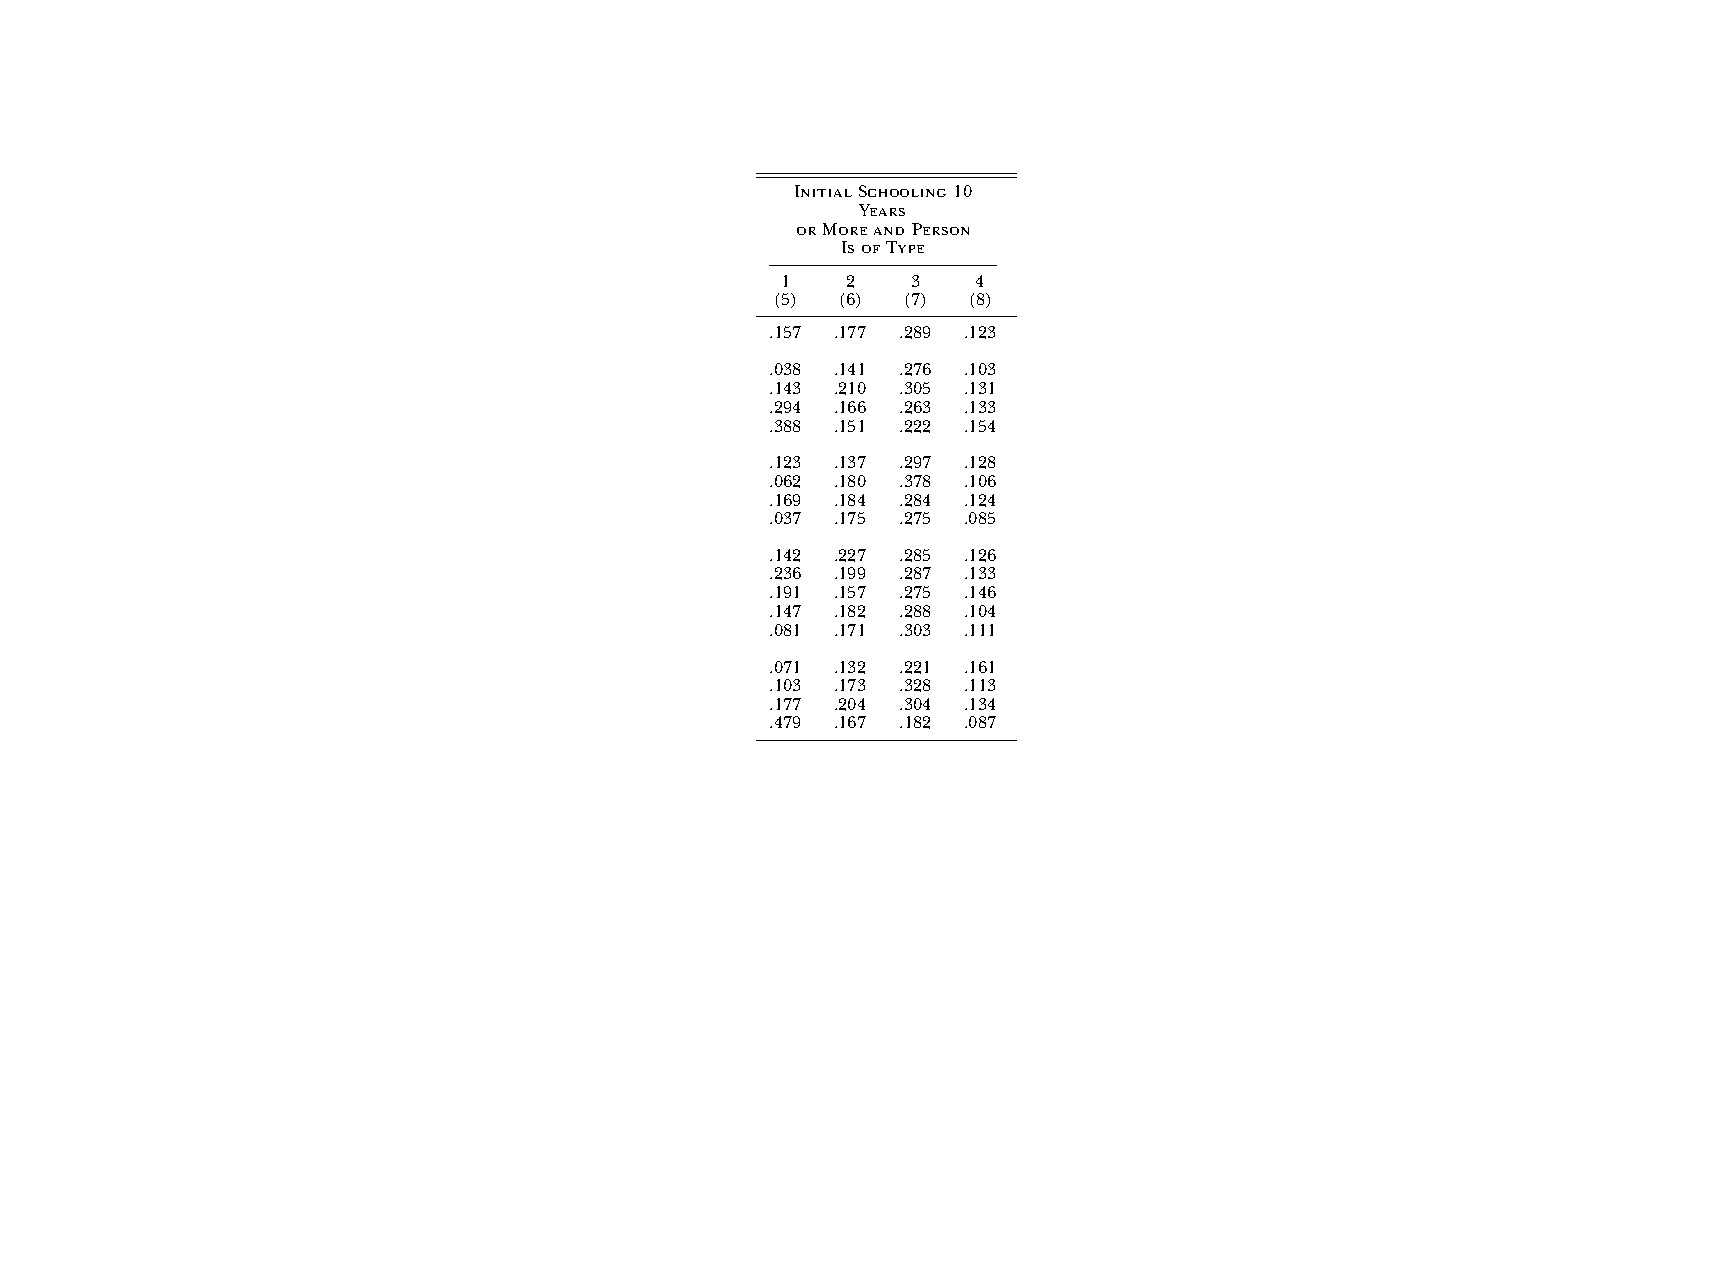
\includegraphics[height=2.75in]{tab-figs/table13b_1997}	\\
	
\includegraphics{tab-figs/table13_1997_footer}	
	\end{center}
\end{frame}

\begin{frame}
	\frametitle{Family Background (contd): Males}
	
\includegraphics[width=\textwidth]{tab-figs/table13_1997_header}	\\
	\begin{center}
	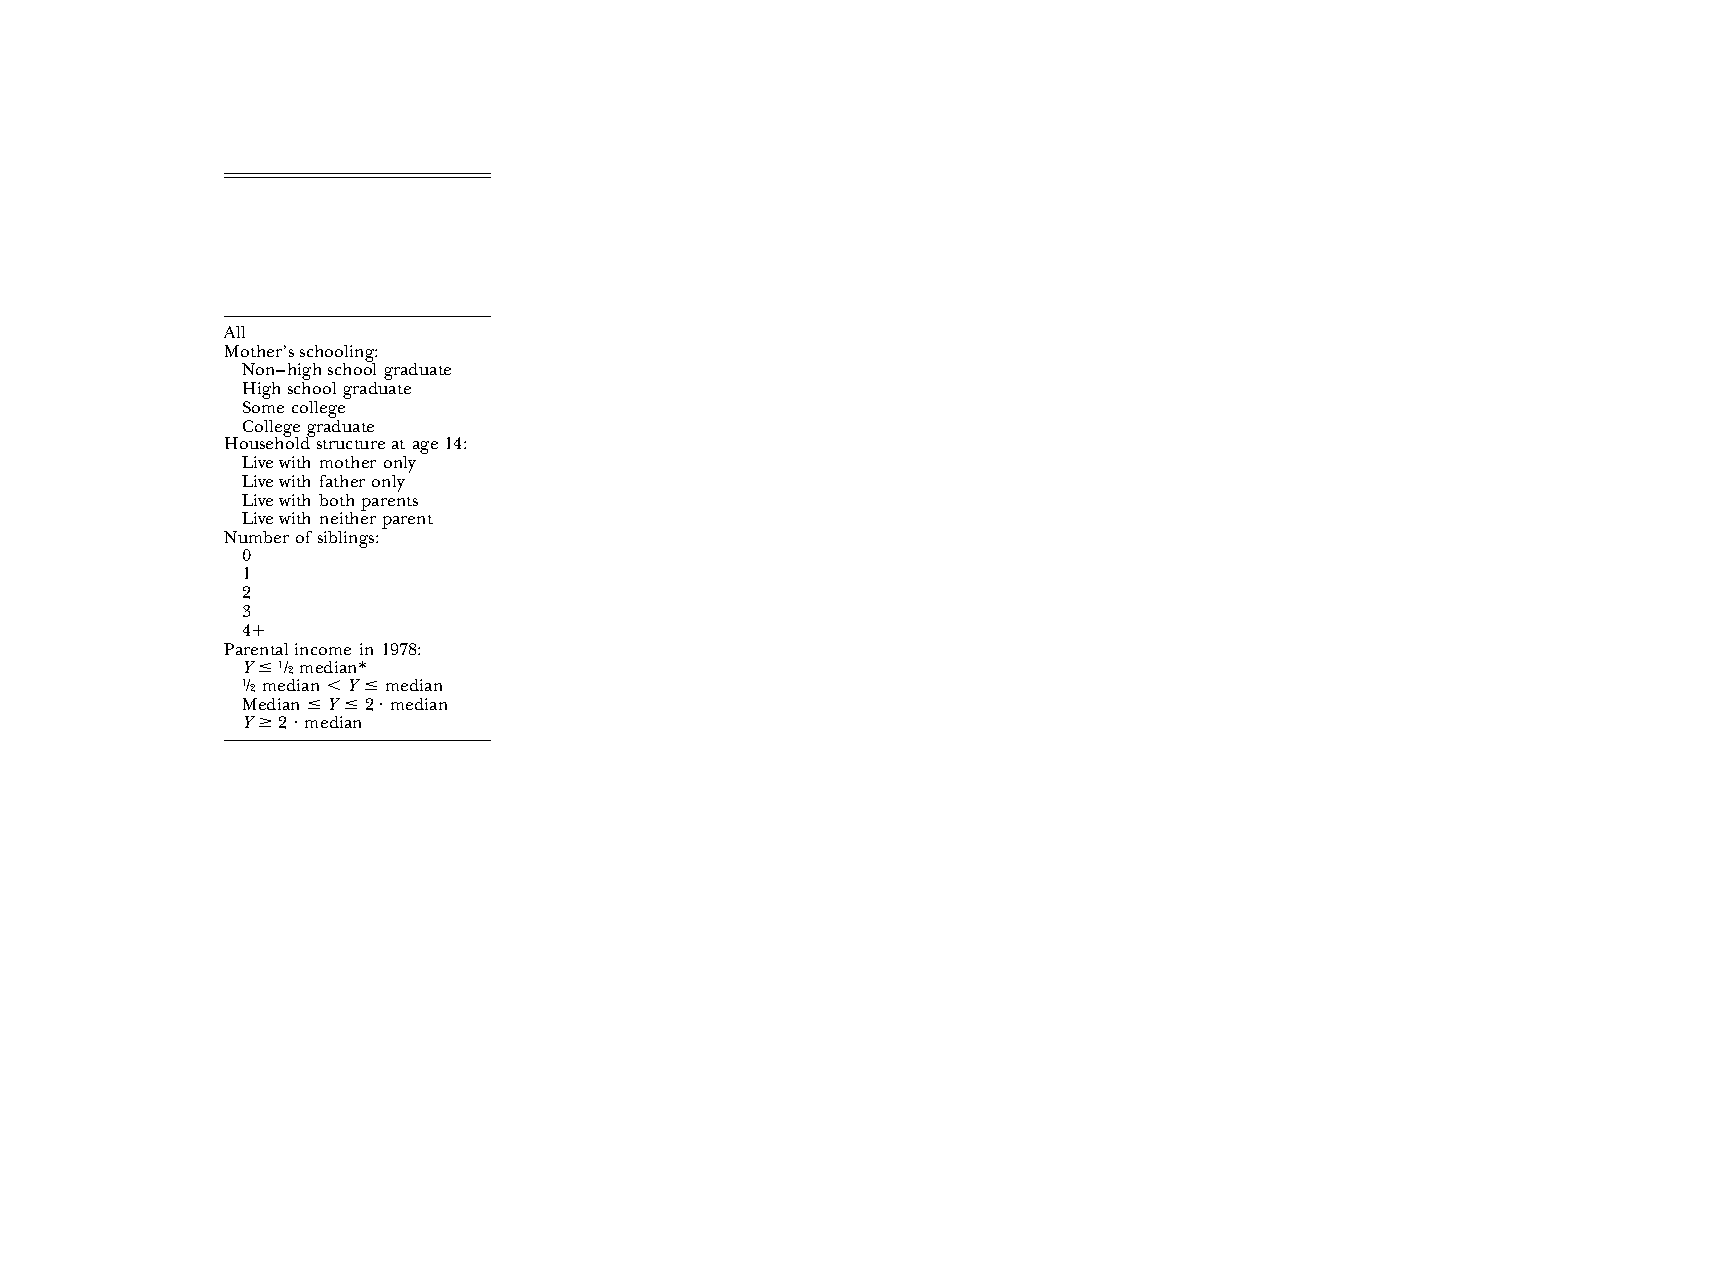
\includegraphics[height=2.75in]{tab-figs/table13_1997_left} 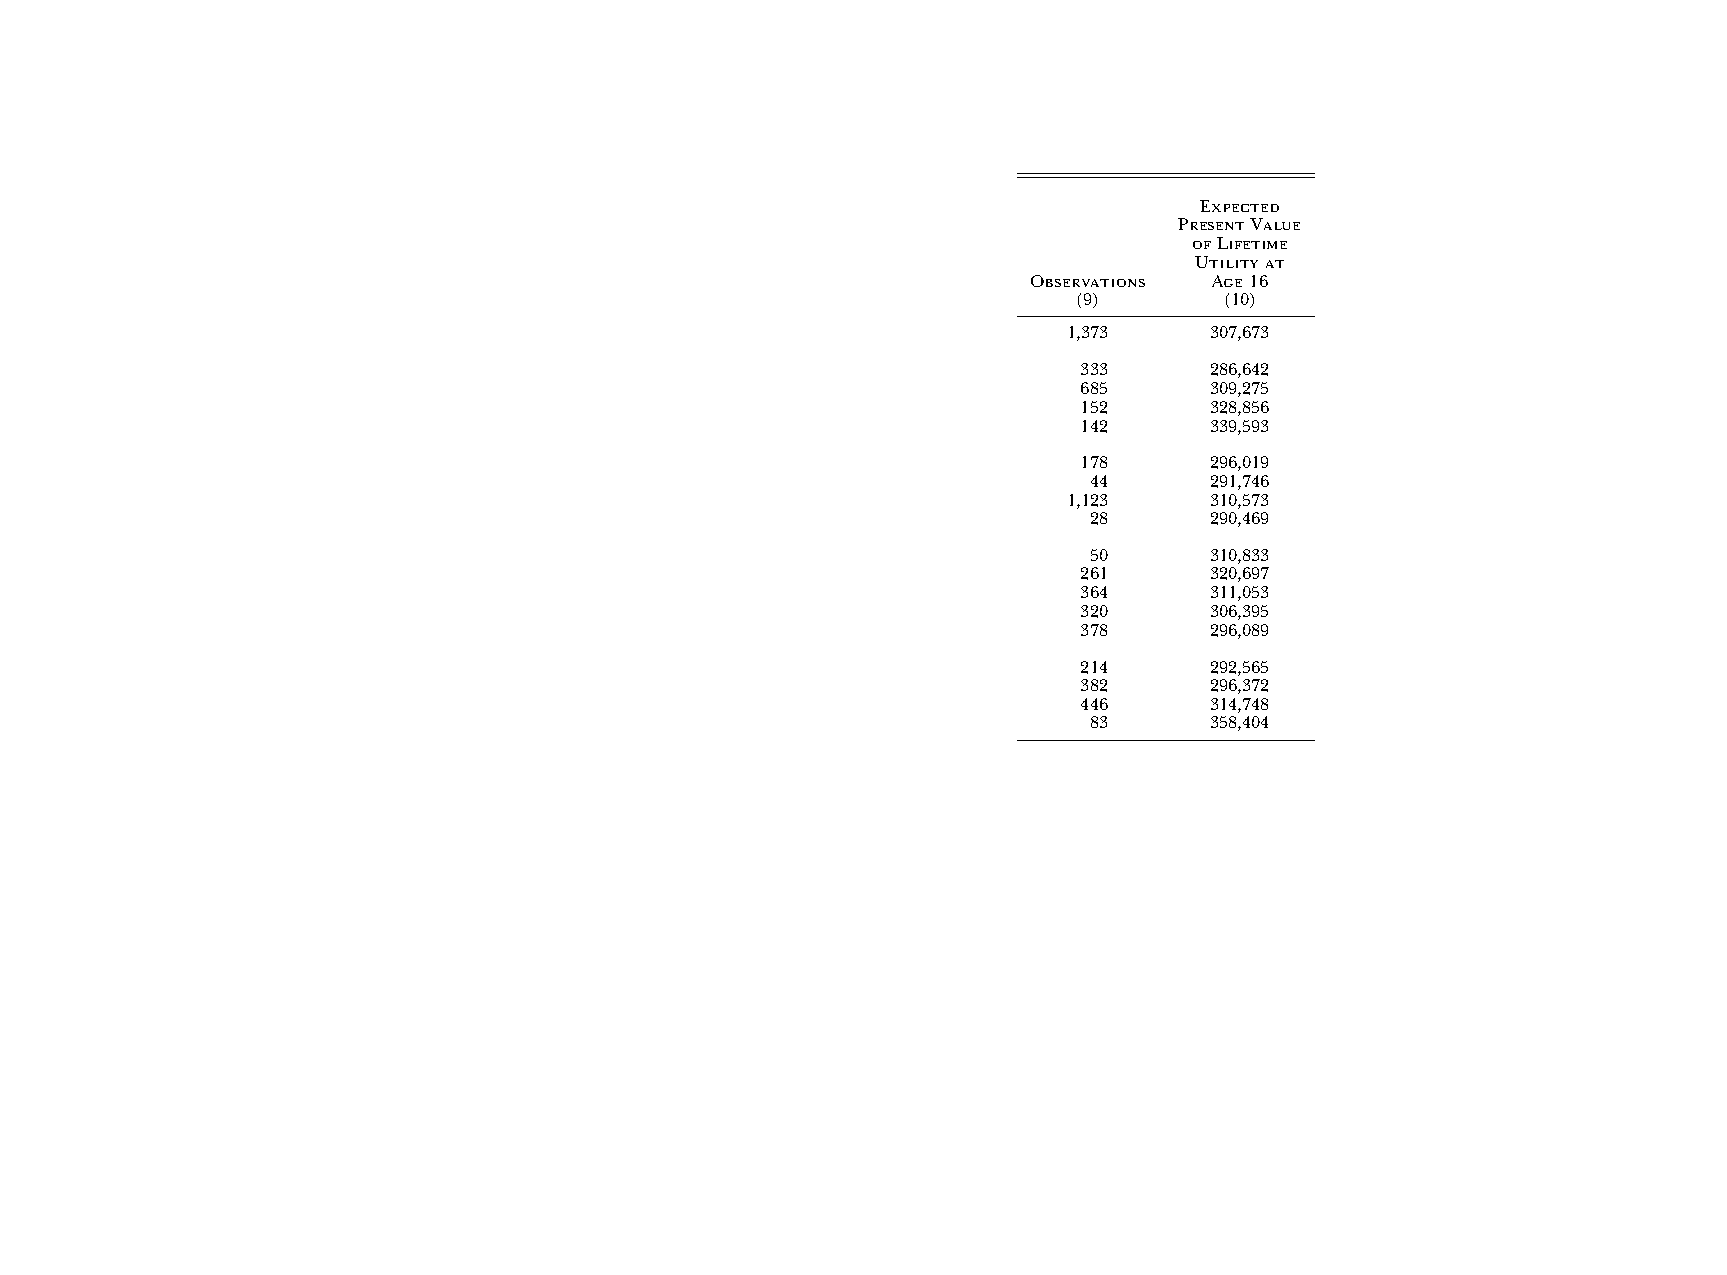
\includegraphics[height=2.75in]{tab-figs/table13c_1997}	\\
	\includegraphics{tab-figs/table13_1997_footer}	
	\end{center}
\end{frame}

\section{Counter-factual Exercises}

\begin{frame}
	\frametitle{Counter-factual Exercises: Females}
		\begin{enumerate}
			\item Equate wage offers, welfare stigma, and parent schooling of blacks and Hispanics to that of whites 
			\item Welfare experiments for ``type 6'' black, Hispanic, and white women 
			\item Increase the wage rate for ``type 6'' black, Hispanic, and white women
			\item Introduction of EITC:
				\begin{itemize}
					\item Unexpected in 2004 for ``type 6'' women
					\item Fully adjusted (in $\Omega_{14}$) in 2004 for ``type 6''
				\end{itemize}							
		\end{enumerate}
\end{frame}

\begin{frame}
	\frametitle{Equating Opportunities for Blacks: Females}
		\includegraphics[width=\textwidth]{tab-figs/table5a_2010_header} \\
		\includegraphics[width=\textwidth]{tab-figs/table5a-a_2010} \\
		\includegraphics[width=\textwidth]{tab-figs/table5a_2010_footer}
\end{frame}

\begin{frame}
	\frametitle{\begin{small}Equating Opportunities for Blacks (contd 1): Females\end{small}}
		\includegraphics[width=\textwidth]{tab-figs/table5a_2010_header} \\
		\includegraphics[width=\textwidth]{tab-figs/table5a-b_2010} \\
		\includegraphics[width=\textwidth]{tab-figs/table5a_2010_footer}
\end{frame}

\begin{frame}
	\frametitle{\begin{small}Equating Opportunities for Blacks (contd 2): Females\end{small}}
		\includegraphics[width=\textwidth]{tab-figs/table5a_2010_header} \\
		\includegraphics[width=\textwidth]{tab-figs/table5a-c_2010} \\
		\includegraphics[width=\textwidth]{tab-figs/table5a_2010_footer}
\end{frame}

\begin{frame}
	\frametitle{Equating Opportunities for Hispanics: Females}
		\includegraphics[width=\textwidth]{tab-figs/table5b_2010_header} \\
		\includegraphics[width=\textwidth]{tab-figs/table5b-a_2010} \\
		\includegraphics[width=\textwidth]{tab-figs/table5b_2010_footer}
\end{frame}

\begin{frame}
	\frametitle{\begin{small}Equating Opportunities for Hispanics (contd 1): Females\end{small}}
		\includegraphics[width=\textwidth]{tab-figs/table5b_2010_header} \\
		\includegraphics[width=\textwidth]{tab-figs/table5b-b_2010} \\
		\includegraphics[width=\textwidth]{tab-figs/table5b_2010_footer}
\end{frame}

\begin{frame}
	\frametitle{\begin{small}Equating Opportunities for Hispanics (contd 2): Females\end{small}}
		\includegraphics[width=\textwidth]{tab-figs/table5b_2010_header} \\
		\includegraphics[width=\textwidth]{tab-figs/table5b-c_2010} \\
		\includegraphics[width=\textwidth]{tab-figs/table5b_2010_footer}
\end{frame}

\begin{frame}
	\frametitle{\begin{small} Welfare Experiments and Wage Increase for Blacks: Females \end{small}}
		\includegraphics[width=\textwidth]{tab-figs/table6a_2010_header} \\
		\includegraphics[width=\textwidth]{tab-figs/table6a-a_2010} \\
		\includegraphics[width=\textwidth]{tab-figs/table6a_2010_footer}
\end{frame}

\begin{frame}
	\frametitle{\begin{small} Welfare Experiments and Wage Increase for Blacks (contd 1): Females \end{small}}
		\includegraphics[width=\textwidth]{tab-figs/table6a_2010_header} \\
		\includegraphics[width=\textwidth]{tab-figs/table6a-b_2010} \\
		\includegraphics[width=\textwidth]{tab-figs/table6a_2010_footer}
\end{frame}

\begin{frame}
	\frametitle{\begin{small} Welfare Experiments and Wage Increase for Blacks (contd 2): Females \end{small}}
		\includegraphics[width=\textwidth]{tab-figs/table6a_2010_header} \\
		\includegraphics[width=\textwidth]{tab-figs/table6a-c_2010} \\
		\includegraphics[width=\textwidth]{tab-figs/table6a_2010_footer}
\end{frame}

\begin{frame}
	\frametitle{\begin{small} Welfare Experiments and Wage Increase for Blacks (contd 3): Females \end{small}}
		\includegraphics[width=\textwidth]{tab-figs/table6a_2010_header} \\
		\includegraphics[width=\textwidth]{tab-figs/table6a-d_2010} \\
		\includegraphics[width=\textwidth]{tab-figs/table6a_2010_footer}
\end{frame}

\begin{frame}
	\frametitle{\begin{small} Welfare Experiments and Wage Increase for Blacks (contd 4): Females \end{small}}
		\includegraphics[width=\textwidth]{tab-figs/table6a_2010_header} \\
		\includegraphics[width=\textwidth]{tab-figs/table6a-e_2010} \\
		\includegraphics[width=\textwidth]{tab-figs/table6a_2010_footer}
\end{frame}

\begin{frame}
	\frametitle{\begin{small} Welfare Experiments and Wage Increase for Hispanics: Females \end{small}}
		\includegraphics[width=\textwidth]{tab-figs/table6b_2010_header} \\
		\includegraphics[width=\textwidth]{tab-figs/table6b-a_2010} \\
		\includegraphics[width=\textwidth]{tab-figs/table6b_2010_footer}
\end{frame}

\begin{frame}
	\frametitle{\begin{small} Welfare Experiments and Wage Increase for Hispanics (contd 1): Females \end{small}}
		\includegraphics[width=\textwidth]{tab-figs/table6b_2010_header} \\
		\includegraphics[width=\textwidth]{tab-figs/table6b-b_2010} \\
		\includegraphics[width=\textwidth]{tab-figs/table6b_2010_footer}
\end{frame}

\begin{frame}
	\frametitle{\begin{small} Welfare Experiments and Wage Increase for Hispanics (contd 2): Females \end{small}}
		\includegraphics[width=\textwidth]{tab-figs/table6b_2010_header} \\
		\includegraphics[width=\textwidth]{tab-figs/table6b-c_2010} \\
		\includegraphics[width=\textwidth]{tab-figs/table6b-d_2010} \\
		\includegraphics[width=\textwidth]{tab-figs/table6b_2010_footer}
\end{frame}

\begin{frame}
	\frametitle{\begin{small} Welfare Experiments and Wage Increase for Hispanics (contd 3): Females \end{small}}
		\includegraphics[width=\textwidth]{tab-figs/table6b_2010_header} \\
		\includegraphics[width=\textwidth]{tab-figs/table6b-e_2010} \\
		\includegraphics[width=\textwidth]{tab-figs/table6b_2010_footer}
\end{frame}

\begin{frame}
	\frametitle{\begin{small} Welfare Experiments and Wage Increase for Hispanics (contd 4): Females \end{small}}
		\includegraphics[width=\textwidth]{tab-figs/table6b_2010_header} \\
		\includegraphics[width=\textwidth]{tab-figs/table6b-f_2010} \\
		\includegraphics[width=\textwidth]{tab-figs/table6b_2010_footer}
\end{frame}

\begin{frame}
	\frametitle{\begin{small} Welfare Experiments and Wage Increase for Whites: Females \end{small}}
		\includegraphics[width=\textwidth]{tab-figs/table6c_2010_header} \\
		\includegraphics[width=\textwidth]{tab-figs/table6c-a_2010} \\
		\includegraphics[width=\textwidth]{tab-figs/table6c_2010_footer}
\end{frame}

\begin{frame}
	\frametitle{\begin{small} Welfare Experiments and Wage Increase for Whites (contd 1): Females \end{small}}
		\includegraphics[width=\textwidth]{tab-figs/table6c_2010_header} \\
		\includegraphics[width=\textwidth]{tab-figs/table6c-b_2010} \\
		\includegraphics[width=\textwidth]{tab-figs/table6c_2010_footer}
\end{frame}

\begin{frame}
	\frametitle{\begin{small} Welfare Experiments and Wage Increase for Whites (contd 2): Females \end{small}}
		\includegraphics[width=\textwidth]{tab-figs/table6c_2010_header} \\
		\includegraphics[width=\textwidth]{tab-figs/table6c-c_2010} \\
		\includegraphics[width=\textwidth]{tab-figs/table6c_2010_footer}
\end{frame}

\begin{frame}
	\frametitle{\begin{small} Welfare Experiments and Wage Increase for Whites (contd 3): Females \end{small}}
		\includegraphics[width=\textwidth]{tab-figs/table6c_2010_header} \\
		\includegraphics[width=\textwidth]{tab-figs/table6c-d_2010} \\
		\includegraphics[width=\textwidth]{tab-figs/table6c_2010_footer}
\end{frame}

\begin{frame}
	\frametitle{\begin{small} Welfare Experiments and Wage Increase for Whites (contd 4): Females \end{small}}
		\includegraphics[width=\textwidth]{tab-figs/table6c_2010_header} \\
		\includegraphics[width=\textwidth]{tab-figs/table6c-e_2010} \\
		\includegraphics[width=\textwidth]{tab-figs/table6c_2010_footer}
\end{frame}


\begin{frame}
	\frametitle{Introduction of EITC: Females}
		\includegraphics[width=\textwidth]{tab-figs/table7_2010}
\end{frame}

\begin{frame}
	\frametitle{Counter-factual Exercises: Males}
		\begin{enumerate}
			\item The impact of college tuition subsidies on school attainment and inequality
		\end{enumerate}
\end{frame}

\begin{frame}
	\frametitle{Effects of a College Subsidy: Males}
		\includegraphics{tab-figs/table14_1997}
\end{frame}

\begin{frame}
	\frametitle{Effects of a College Subsidy (contd): Males}
		\includegraphics{tab-figs/table15_1997}
\end{frame}

\end{document}